\documentclass[11pt]{book}
\usepackage{fullpage}
\usepackage{palatino}
\usepackage{amsfonts,amsmath,amssymb}

% Packages for displaying code:
\usepackage{listings}
\usepackage{textcomp}
\usepackage{color}

% Color settings used in the code below:
\definecolor{dkgreen}{rgb}{0,0.6,0}
\definecolor{gray}{rgb}{0.5,0.5,0.5}
\definecolor{mauve}{rgb}{0.58,0,0.82}

% Settings for the formatting of the code on display:
\lstset{frame=tb,
  language=R,
  aboveskip=3mm,
  belowskip=3mm,
  showstringspaces=false,
  columns=flexible,
  basicstyle={\small\ttfamily},
  numbers=none,
  numberstyle=\tiny\color{gray},
  keywordstyle=\color{blue},
  commentstyle=\color{dkgreen},
  stringstyle=\color{mauve},
  breaklines=true,
  breakatwhitespace=true,
  tabsize=3
}

% Packages for Figures:
% Without conversion of eps to pdf:
% \usepackage{graphicx}
% With conversion of eps to pdf,
% which depends on platform.
\ifx\pdftexversion\undefined
    \usepackage[dvips]{graphicx}
\else
    \usepackage[pdftex]{graphicx}
    \usepackage{epstopdf}
    \epstopdfsetup{suffix=}
\fi

\usepackage{subfig}

% Package for displaying inline verbatim commands in footnotes.
\usepackage{fancyvrb}

% This allows pdflatex to print the curly quotes in the
% significance codes in the output of the GAM.
\UseRawInputEncoding

%%%%%%%%%%%%%%%%%%%%%%%%%%%%%%%%%%%%%%%%
\begin{document}
%%%%%%%%%%%%%%%%%%%%%%%%%%%%%%%%%%%%%%%%



\pagestyle{empty}
{\noindent\bf Spring 2021 \hfill Firstname M.~Lastname}
\vskip 16pt
\centerline{\bf University of Central Florida}
\centerline{\bf College of Business}
\vskip 16pt
\centerline{\bf QMB 6911}
\centerline{\bf Capstone Project in Business Analytics}
\vskip 10pt
\centerline{\bf Solutions:  Problem Set \#11}
\vskip 32pt
\noindent



\pagebreak
\chapter{Introduction}
%\documentclass[11pt]{book}
%\usepackage{palatino}
%\usepackage{amsfonts,amsmath,amssymb}
%
%\begin{document}
%\pagestyle{empty}
%{\noindent\bf Spring 2022 \hfill Firstname M.~Lastname}
%\vskip 16pt
%\centerline{\bf University of Central Florida}
%\centerline{\bf College of Business}
%\vskip 16pt
%\centerline{\bf QMB 6912}
%\centerline{\bf Capstone Project in Business Analytics}
%\vskip 10pt
%\centerline{\bf Solutions:  Problem Sets \#1 \& 2}
%\vskip 32pt
%
%This example has sections for each article in Problem Set \#1.

\section{Introduction}

In this paper I analyze the prices of fly reels. 
My aim is to investigate the value of fly reels produced in different locations.
Does there exist a Made-in-America premium? 
If so, how large is it?
Does the premium depend on the characteristics of the fly reels?
% 
The answers to these questions can be applied to the 
operational decisions of fly reel manufacturers.
In particular, this analysis can be used to make recommendations
on whether fly reels should be made in America or produced overseas. 
% 

In the following pages, I will investigate these questions and
ultimately fit a model for the price of fly reels, 
allowing for endogeneity in the choice of the
characteristics of fly reels 
and the location in which they are manufacturers
produced and sold by each manufacturer. 
To understand the dynamics of a sample selection model, 
it is worthwhile to understand the research related to these questions. 



\section{Economic Theory}

\subsection{Market for Lemons}


Akerlof's description of the market for lemons is a long-standing contribution to the understanding of asymmetric information. 


\subsection{Characteristic Theory}

The paper by Lancaster (1966) is a contribution to economic theory in which he makes the case for a sound theory of consumer choice, 
in which the consumer's preferences are defined on the characteristics of different goods, 
rather than the quantities of uniformly-defined goods.


\subsection{Hedonic Pricing Models}

Rosen (1974) builds on the work of Lancaster (1966)
by providing an empirical framework for estimating the value
of products based on their characteristics. 




\section{Empirical Framework}

\subsection{Tobit Models}

Heckman (1979) described sample selection models as a model specification question. 

Amemiya (1984) summarized the variaous types of Tobit models
and provides a review of research with applications of these models. 

Lee and Trost (1978) is a well-known application to housing markets, 
which incorporates the fact that the residents make a decision
to either own or rent a home before buying. 


% \end{document}

\pagebreak
\chapter{Data Description}
\section{Data Description}


By engaging an industry consultant to gather relevant and appropriate 
information, your firm has been able to put together data concerning 248 
different fly-fishing reels, over one-half of which are produced in the 
United States, with the remainder being produced in Asia---either in China 
or Korea.  These data are contained in the file {\tt FlyReels.csv}, which is
available in the {\tt Data} folder.
Each fly-fishing reel in the data set is a row, while the columns correspond 
to the variables whose names and definitions are the following:

\bigskip
\begin{table}[ht]
\centering
\begin{tabular}{ll}
  \hline
    Variable & Definition \\
  \hline

    {\tt Name}        &product name (a string) \\ 
    {\tt Brand}       &brand name (a string) \\ 
    {\tt Weight}      &weight of reel in ounces (a real number) \\ 
    {\tt Diameter}    &diameter of reel in inches (a real number) \\ 
    {\tt Width}       &width of reel in inches (a real number) \\ 
    {\tt Price}       &price of reel in dollars (a real number) \\ 
    {\tt Sealed}      &whether the reel is sealed; {\tt "Yes"} versus
                        {\tt "No"} (a string) \\ 
    {\tt Country}     &country of manufacture, (a string) \\ 
    {\tt Machined}    &whether the reel is machined versus cast;
                        machined={\tt "Yes"}, \\ 
                      &while cast={\tt "No"} (a string) \\ 
  \hline
\end{tabular}
%\caption{Summary of Numeric Variables}
%\label{tab:summary}
\end{table}


\pagebreak
\chapter{Analysis of the Dependent Variable}
%\documentclass[11pt]{book}
%\usepackage{palatino}
%\usepackage{amsfonts,amsmath,amssymb}
%% \usepackage{graphicx}
%
%
%\ifx\pdftexversion\undefined
%    \usepackage[dvips]{graphicx}
%\else
%    \usepackage[pdftex]{graphicx}
%    \usepackage{epstopdf}
%    \epstopdfsetup{suffix=}
%\fi
%
%
%\begin{document}

%%%%%%%%%%%%%%%%%%%%%%%%%%%%%%%%%%%%%%%%
% Problem Set 4
%%%%%%%%%%%%%%%%%%%%%%%%%%%%%%%%%%%%%%%%

%\pagestyle{empty}
%{\noindent\bf Spring 2021 \hfill Firstname M.~Lastname}
%\vskip 16pt
%\centerline{\bf University of Central Florida}
%\centerline{\bf College of Business}
%\vskip 16pt
%\centerline{\bf QMB 6911}
%\centerline{\bf Capstone Project in Business Analytics}
%\vskip 10pt
%\centerline{\bf Solutions:  Problem Set \#4}
%\vskip 32pt
%\noindent



\section{Empirical Distribution Function of Fly Reel Prices}

Figure \ref{fig:ecdf_prices} is 
a plot of the empirical cumulative distribution function (CDF) of fly reel prices. 


\begin{figure}[h!]
  \centering
  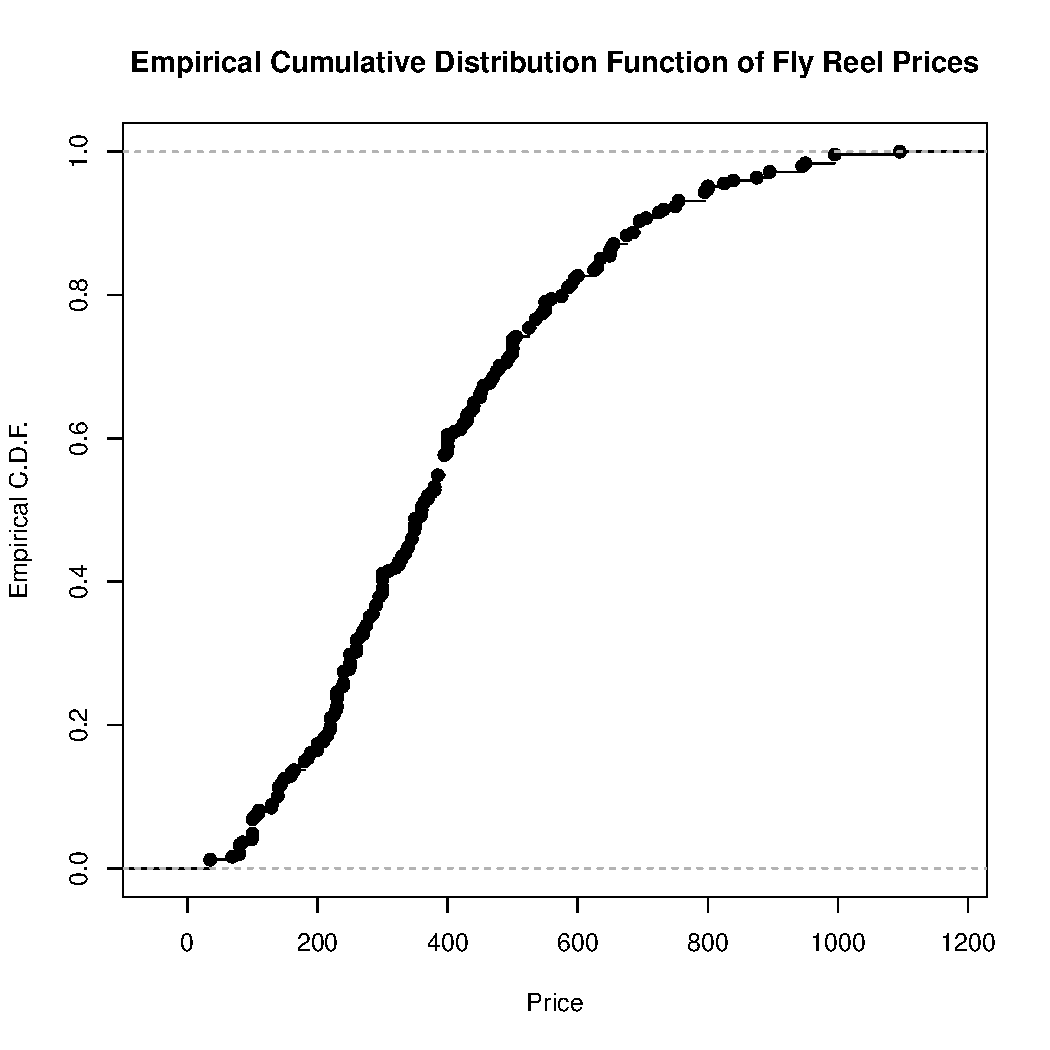
\includegraphics[scale = 0.5, keepaspectratio=true]{../Figures/ecdf_prices}
  \caption{Empirical Distribution Function of Fly Reel Prices} \label{fig:ecdf_prices}
\end{figure}


\section{Relative Histogram of Fly Reel Prices}

Figure \ref{fig:hist_prices} is 
a histogram of fly reel prices. 

\begin{figure}[h!]
  \centering
  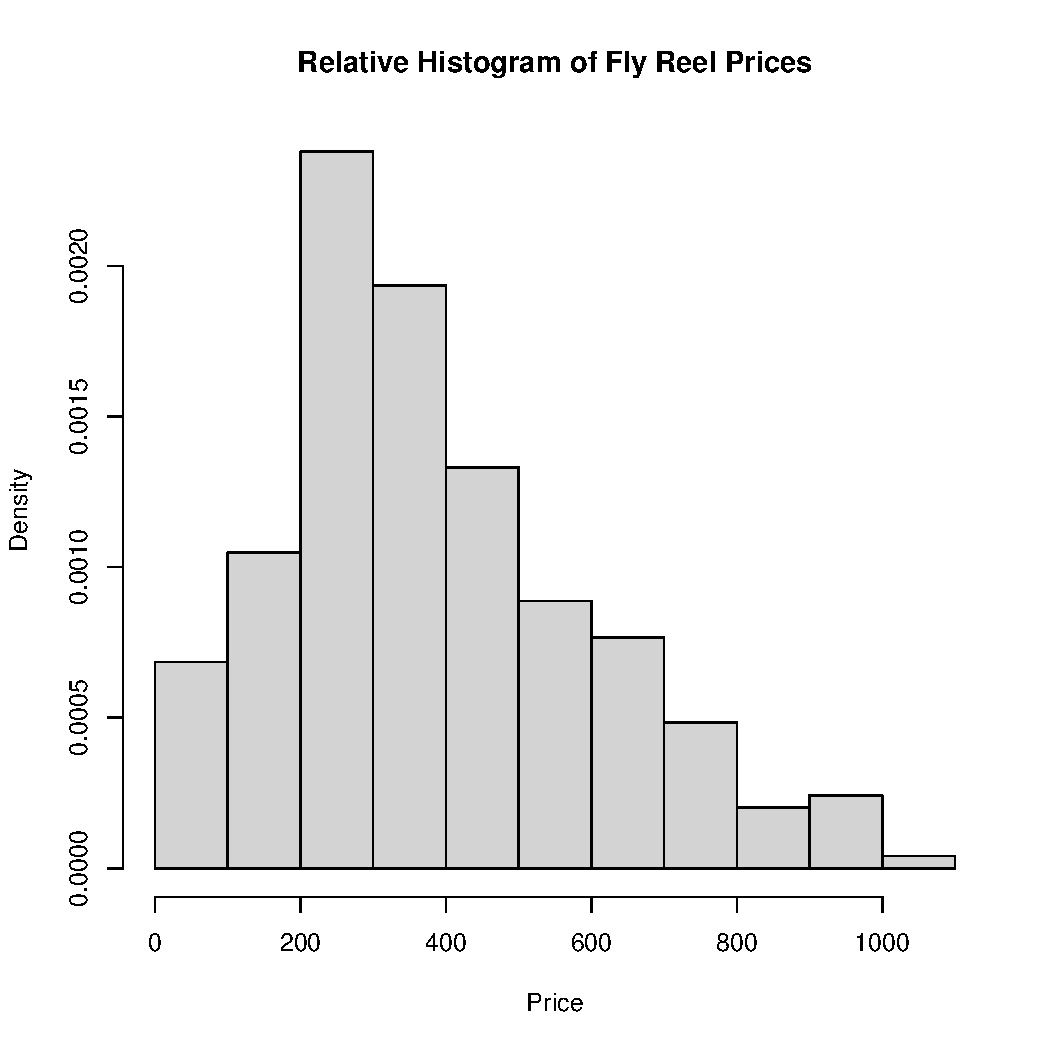
\includegraphics[scale = 0.5, keepaspectratio=true]{../Figures/hist_prices}
  \caption{Relative Histogram of Fly Reel Prices} \label{fig:hist_prices}
\end{figure}


\pagebreak
\section{Probability Density Function of Fly Reel Prices}

Figure \ref{fig:density_prices} depicts 
the kernel-smoothed probability density function of the natural logarithm of
price.

\begin{figure}[h!]
  \centering
  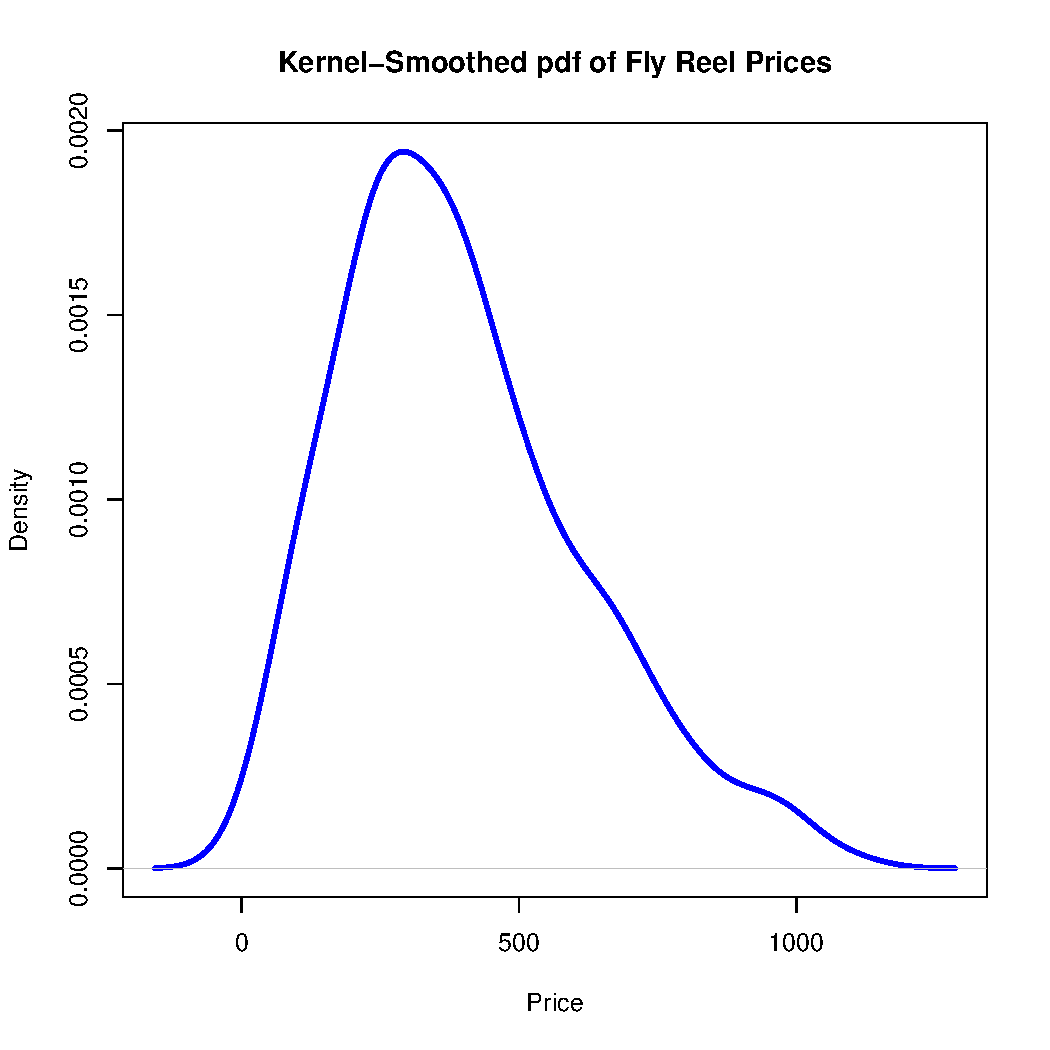
\includegraphics[scale = 0.5, keepaspectratio=true]{../Figures/density_prices}
  \caption{Probability Density Function of Fly Reel Prices} \label{fig:density_prices}
\end{figure}



%%%%%%%%%%%%%%%%%%%%%%%%%%%%%%%%%%%%%%%%
% \end{document}
%%%%%%%%%%%%%%%%%%%%%%%%%%%%%%%%%%%%%%%%


\pagebreak
\chapter{Transforming the Dependent Variable}
\documentclass[11pt]{book}
\usepackage{palatino}
\usepackage{amsfonts,amsmath,amssymb}
% \usepackage{graphicx}

\usepackage{listings}
\usepackage{textcomp}
\usepackage{color}

\definecolor{dkgreen}{rgb}{0,0.6,0}
\definecolor{gray}{rgb}{0.5,0.5,0.5}
\definecolor{mauve}{rgb}{0.58,0,0.82}

\lstset{frame=tb,
  language=R,
  aboveskip=3mm,
  belowskip=3mm,
  showstringspaces=false,
  columns=flexible,
  basicstyle={\small\ttfamily},
  numbers=none,
  numberstyle=\tiny\color{gray},
  keywordstyle=\color{blue},
  commentstyle=\color{dkgreen},
  stringstyle=\color{mauve},
  breaklines=true,
  breakatwhitespace=true,
  tabsize=3
}



\ifx\pdftexversion\undefined
    \usepackage[dvips]{graphicx}
\else
    \usepackage[pdftex]{graphicx}
    \usepackage{epstopdf}
    \epstopdfsetup{suffix=}
\fi

\usepackage{subfig}

\begin{document}

%%%%%%%%%%%%%%%%%%%%%%%%%%%%%%%%%%%%%%%%
% Problem Set 6
%%%%%%%%%%%%%%%%%%%%%%%%%%%%%%%%%%%%%%%%

\pagestyle{empty}
{\noindent\bf Spring 2023 \hfill Firstname M.~Lastname}
\vskip 16pt
\centerline{\bf University of Central Florida}
\centerline{\bf College of Business}
\vskip 16pt
\centerline{\bf QMB 6911}
\centerline{\bf Capstone Project in Business Analytics}
\vskip 10pt
\centerline{\bf Solutions:  Problem Set \#3}
\vskip 32pt
\noindent


%%%%%%%%%%%%%%%%%%%%%%%%%%%%%%%%%%%%%%%%
% Density Plots and Q-Q Plots
%%%%%%%%%%%%%%%%%%%%%%%%%%%%%%%%%%%%%%%%


\pagebreak
\section*{Probability Density Function of Fly Reel Prices}

Figure \ref{fig:density_prices} shows  the kernel-smoothed probability density function of fly reel prices.

\begin{figure}[h!]
  \centering
  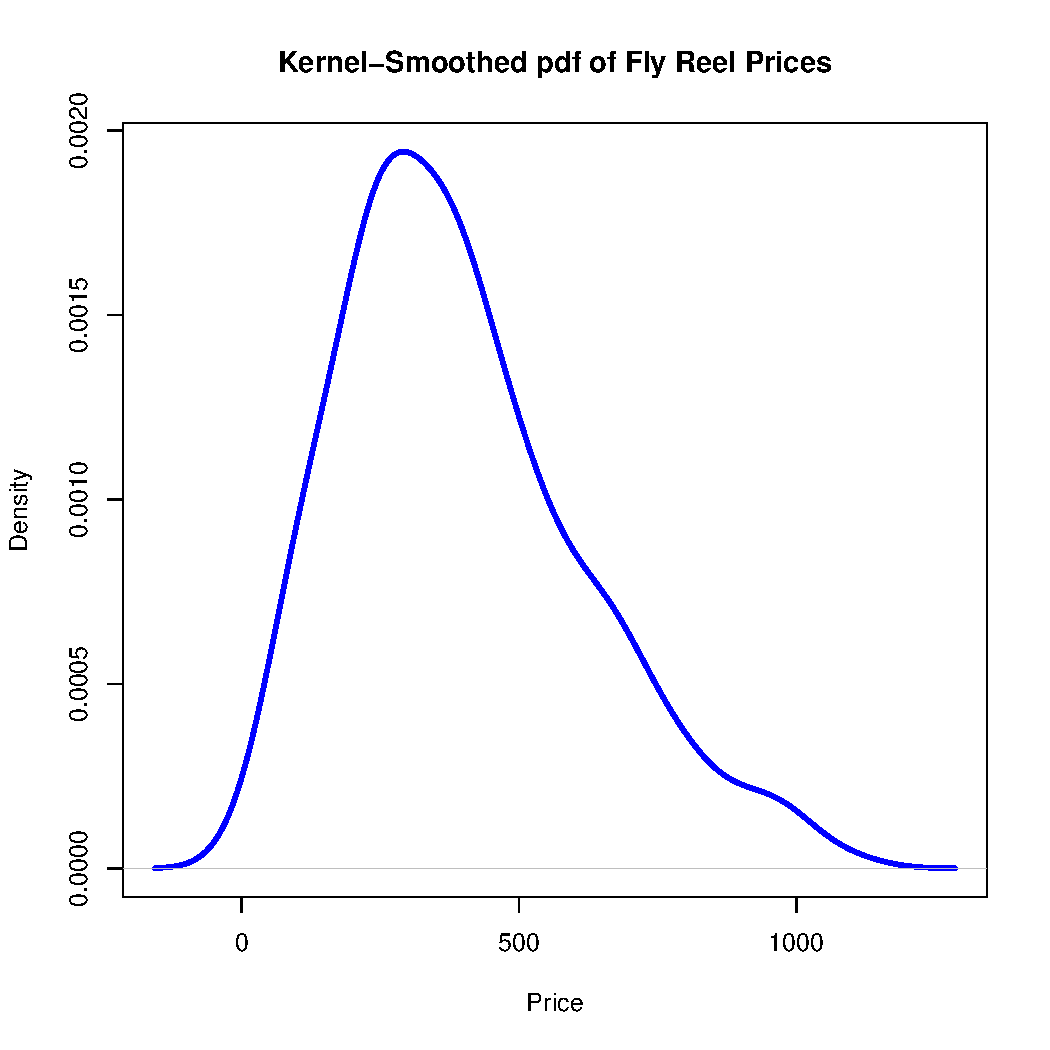
\includegraphics[scale = 0.5, keepaspectratio=true]{../Figures/density_prices}
  \caption{Probability Density Function of Fly Reel Prices} \label{fig:density_prices}
\end{figure}



\pagebreak
As a comparison, Figure \ref{fig:density_log_prices} shows the kernel-smoothed probability density function of the natural logarithm of
price.

\begin{figure}[h!]
  \centering
  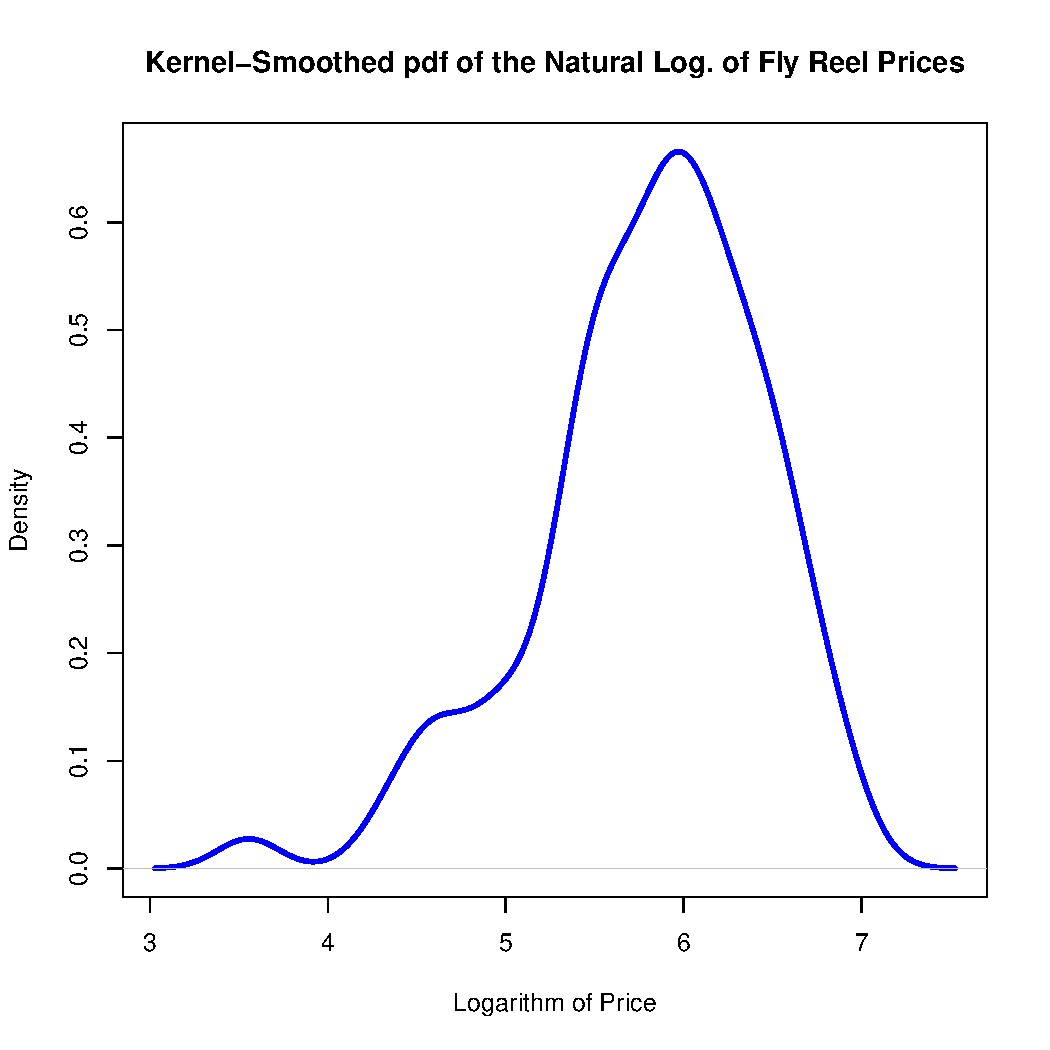
\includegraphics[scale = 0.5, keepaspectratio=true]{../Figures/density_log_prices}
  \caption{Probability Density Function of the Logarithm of Fly Reel Prices} \label{fig:density_log_prices}
\end{figure}




\pagebreak
\section*{Normality of the Original and Transformed Variables}

Figure \ref{fig:qq_prices} shows a pair of Q-Q plots, 
comparing quantiles of the empirical distribution against
the quantiles of the normal distribution. 
In the left panel, Figure \ref{subfig:qq_prices} shows this comparison 
for the original level of the fly reel prices, without transformation. 
In the right panel, Figure \ref{subfig:qq_log_prices} shows this comparison 
for the logarithmic transformation of fly reel prices, without transformation. 
Consistent with the pair of distributions estimated above, 
each plot shows a divergence from a normal distribution,
suggesting that an optimal transformation might lie somewhere in the middle.
The Box-Cox transformation allows for this possibility. 

\begin{figure}[!ht]
\subfloat[Fly Reel Prices\label{subfig:qq_prices}]{%
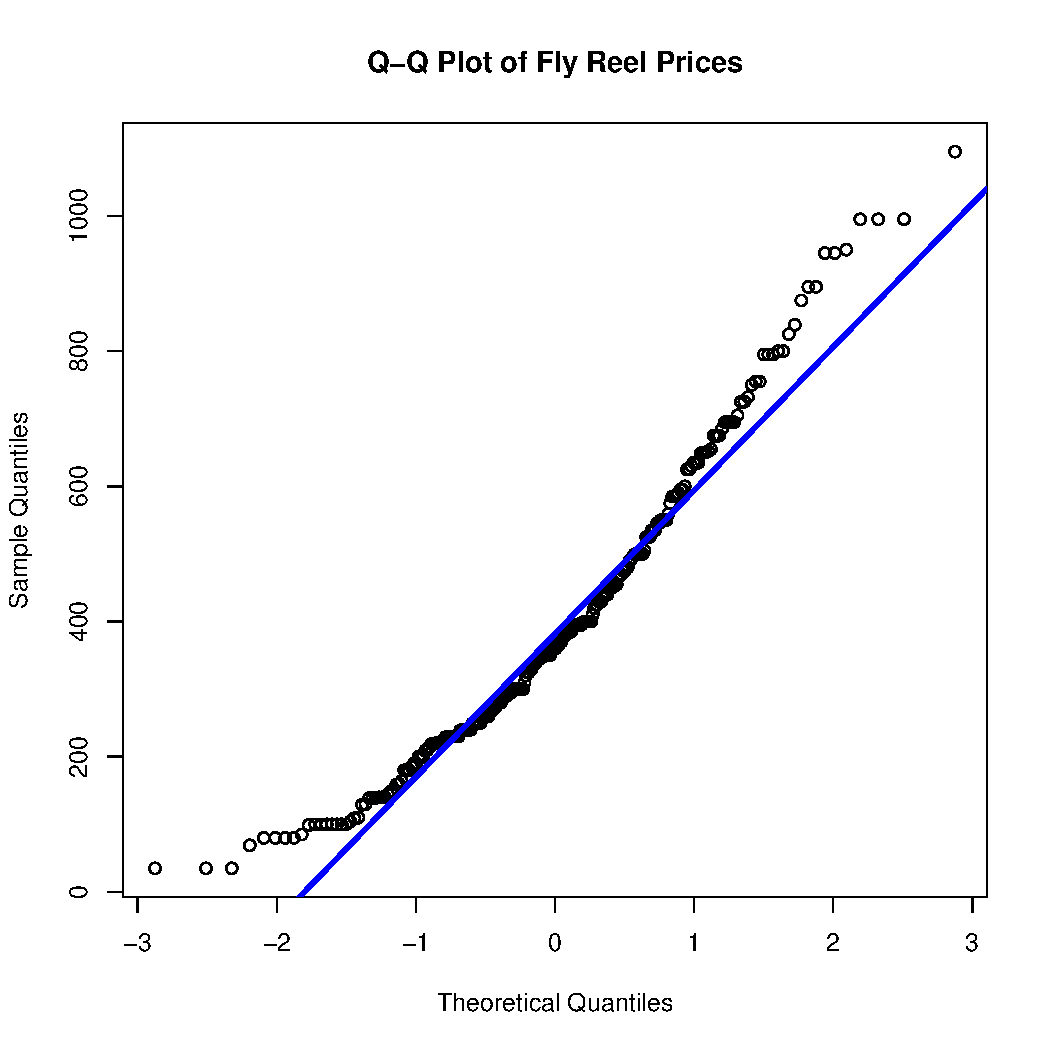
\includegraphics[width=0.5\textwidth]{../Figures/qq_prices}}
\hfill
\subfloat[Transformed Fly Reel Prices\label{subfig:qq_log_prices}]{%
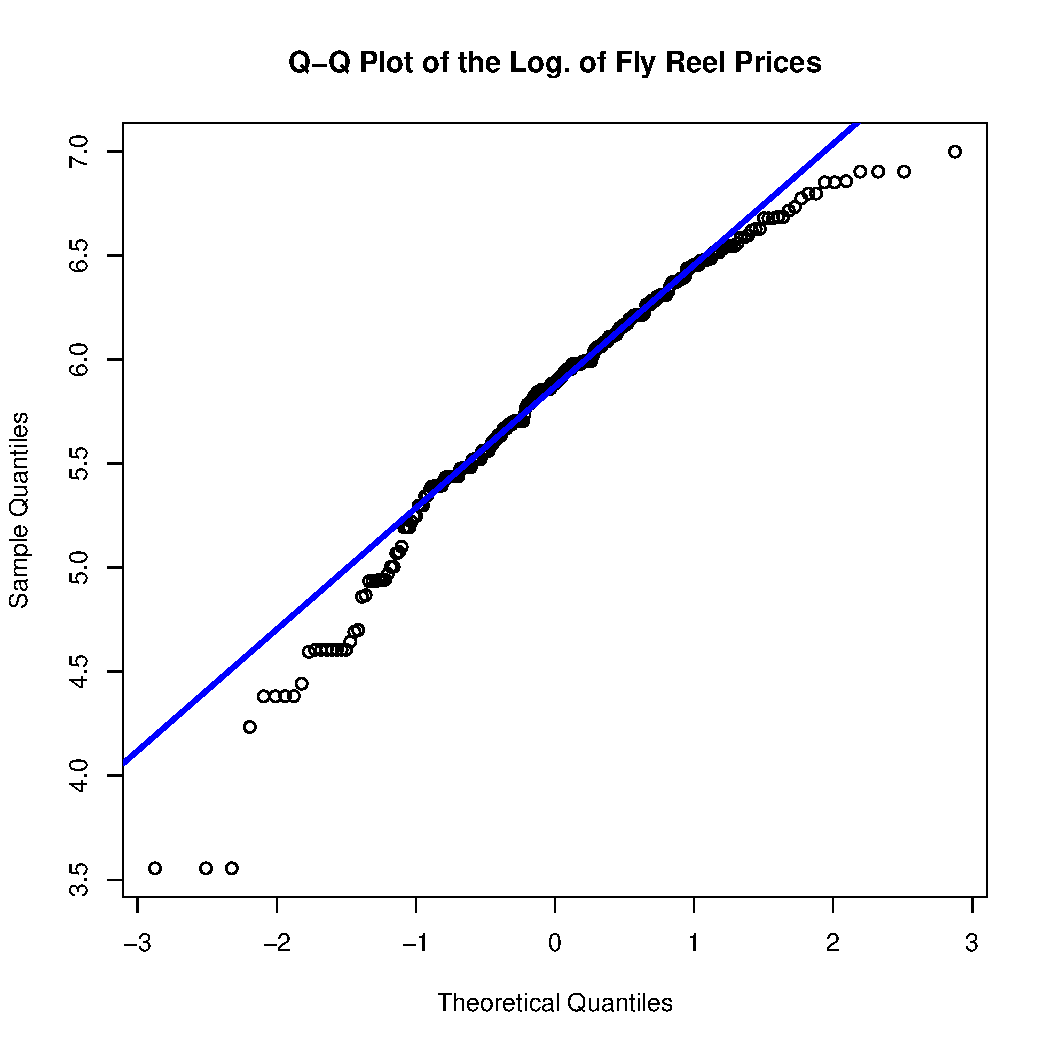
\includegraphics[width=0.5\textwidth]{../Figures/qq_log_prices}}

\caption{Q-QPlots of the Log. and Levels of Fly Reel Prices}
\label{fig:qq_prices}
\end{figure}



%%%%%%%%%%%%%%%%%%%%%%%%%%%%%%%%%%%%%%%%
% Box-Cox Transformation
%%%%%%%%%%%%%%%%%%%%%%%%%%%%%%%%%%%%%%%%


\pagebreak
\section{Box-Cox Transformation of Fly Reel Prices}

Under the Box--Cox transformation of $P_n$, the price of reel $n$
is calculated as follows,
$$\Lambda(P_n)\equiv
  \begin{cases}
	\frac{P_n^\lambda-1}{\lambda}	& \textrm{if } \lambda > 0 \\
           \log P_n                     			& \textrm{if } \lambda = 0.\\
  \end{cases}
$$
The following code block defines a function that performs a
Box-Cox transformation.

\vspace{1.0in}

\begin{lstlisting}[language=R]
# Box-Cox transformation.
Lambda_Price <- function(price, lambda) {
  if (lambda == 0) {
    return(log(price))
  } else {
    return((price^lambda - 1)/lambda)
  }
}
\end{lstlisting}

\pagebreak
\subsection{Log-likelihood Function}

Under the Box-Cox transformation,
the fly reel prices can be decomposed into a location parameter $\mu^0$ 
and an error $U$, so
$$\Lambda(P_n) = \mu^0(\lambda) + U_n,$$
where the $U_n$s are independent, mean-zero, constant-variance 
$\sigma^2(\lambda)$, Gaussian (normal) errors. 
In the above equation, for clarity, the dependence of $\mu^0$ and 
$\sigma^2(\lambda)$ on $\lambda$ is made explicit.


The next code block defines a likelihood function for the normal distribution of the errors
as a function of the parameter $\lambda$.

\begin{lstlisting}[language=R]
log_like_uni <- function(price, lambda) {

  # Calculate maximum likelighood estimates of the parameters.
  n <- length(price)
  lambda_price <- Lambda_Price(price, lambda)
  mu_0_lambda <- mean(lambda_price)
  sigma_2_lambda <- sum((lambda_price - mu_0_lambda)^2)/n

  # Calculate the log-likelihood from the sum of the logarithms
  # of the density of the normal distribution.
  like <- - n/2*log(2*pi*sigma_2_lambda)
  like <- like - 1/2/sigma_2_lambda*sum((lambda_price - mu_0_lambda)^2)
  like <- like + (lambda - 1)*sum(log(price))
  return(like)
}
\end{lstlisting}

\pagebreak
As a first approximation, 
One can calculate the value of the log-likelihood function on a grid of values
to find an optimal value of $\lambda$.
The plot of this likelihood function is shown in Figure \ref{fig:box_cox_loglike_uni}.
The red points represent the values of the log-likelihood 
at the optimum $\lambda = 0.43$ and at $\lambda = 0$ and $\lambda = 1$.

\begin{lstlisting}[language=R]
# Calculate values of the log-likelihood function.
lambda_grid <- seq(-1, 2.5, by = 0.001)
like_grid <- 0*lambda_grid
for (lambda_num in 1:length(lambda_grid)) {
  like_grid[lambda_num] <- log_like_uni(price = flyreels[, 'Price'],
                                    lambda = lambda_grid[lambda_num])
}
\end{lstlisting}

\begin{figure}[h!]
  \centering
  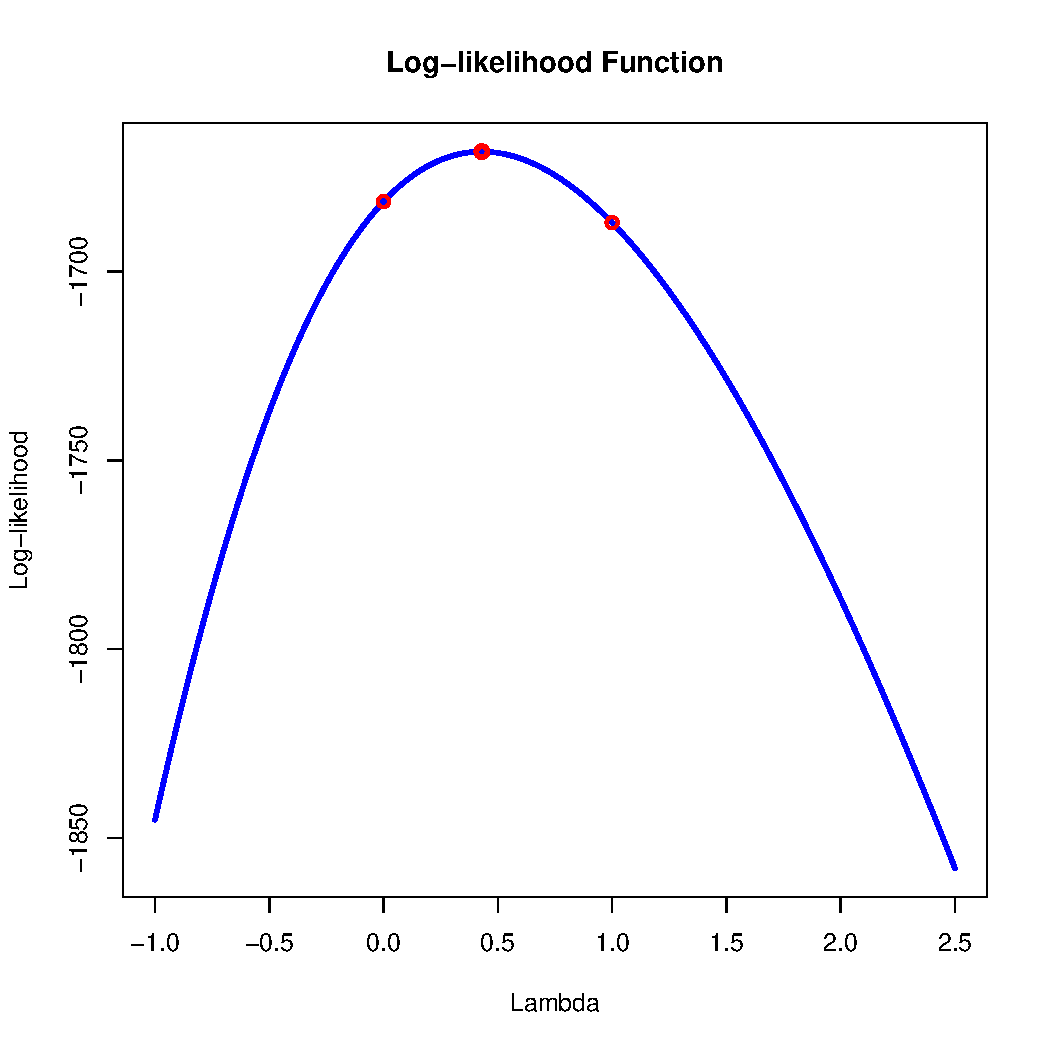
\includegraphics[scale = 0.5, keepaspectratio=true]{../Figures/box_cox_loglike_uni}
  \caption{Log-likelihood Function for Box-Cox Transformation} \label{fig:box_cox_loglike_uni}
\end{figure}


\pagebreak
\subsection{Testing for an Appropriate Transformation}

Now we consider the statistical properties of these estimates
by calculating a likelihood ratio statistic.

\begin{lstlisting}[language=R]
> # Calculate likelihood ratio statistics.
> LR_stat_0 <- - 2*(like_mu_0 - like_MLE)
> print(LR_stat_0)
[1] 26.4604
> LR_stat_1 <- - 2*(like_mu_1 - like_MLE)
> print(LR_stat_1)
[1] 37.62182
> 
> 
> # Compare to quantile of chi-squared distribution with 1 degree of freedom.
> LR_cv_5 <- qchisq(p = 0.95, df = 1)
> print(LR_cv_5)
[1] 3.841459
> 
> # Calculate p-values for these tests.
> p_value_0 <- 1 - pchisq(q = LR_stat_0, df = 1)
> print(p_value_0)
[1] 2.689959e-07
> p_value_1 <- 1 - pchisq(q = LR_stat_1, df = 1)
> print(p_value_1)
[1] 8.58782e-10
> 
\end{lstlisting}

Statistically, this is evidence to reject them both.
This suggests using the transformation at the MLE.
However, one may want to investigate further 
to find out whether it is worth 
transforming the data. 
There exists a trade-of between interpretability and 
the accuracy of the statistical specification. 


\clearpage
\section{\textsf{R} Packages for the Box-Cox Transformation}
\subsection*{Using the \texttt{MASS} Package}

As an illustration, we calculated
the likelihood ourselves.
However, there exist other packages
to output the estimation results for
an optimal Box-Cox transformation.

One option is to use the function from the \texttt{MASS} package.
This is an \textsf{R} package that accompanies a well-know statistics textbook
and has a great reputation. 
In the \texttt{MASS} package, the notation is the same as for a linear model.


\begin{lstlisting}[language=R]
# In the MASS package, the notation is the same as for a linear model.
# i.e., summary(lm(Price ~ 1, data = flyreels))
bc_grid_MASS <- MASS::boxcox(Price ~ 1,
                             data = flyreels,
                             lambda = lambda_grid)
\end{lstlisting}

The output is plotted in Figure \ref{fig:plot_like_MASS}.

\begin{figure}[h!]
  \centering
  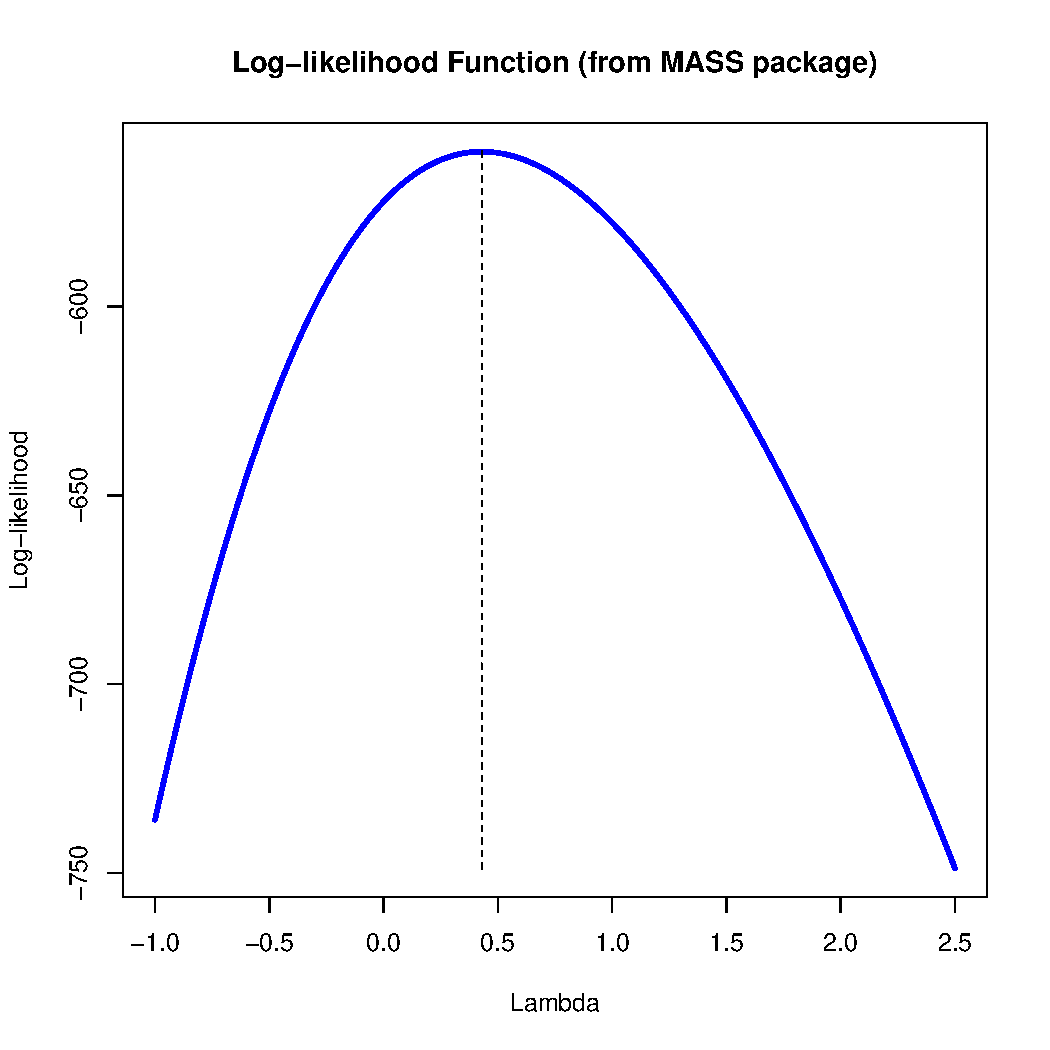
\includegraphics[scale = 0.5, keepaspectratio=true]{../Figures/plot_like_MASS}
  \caption{Log-likelihood Function for Box-Cox Transformation (\texttt{MASS} package)} \label{fig:plot_like_MASS}
\end{figure}


\clearpage
\section*{Using the \texttt{car} Package}

The \texttt{car} package is another well-known option.
With this function, the optimization produces 
a figure automatically from the code below.

\begin{lstlisting}[language=R]
bc_grid_car <- car::boxCox(object = lm(data = flyreels,
                                       formula = Price ~ 1),
                           lambda = lambda_grid)
\end{lstlisting}

The output is plotted in Figure \ref{fig:plot_like_car}.

\begin{figure}[h!]
  \centering
  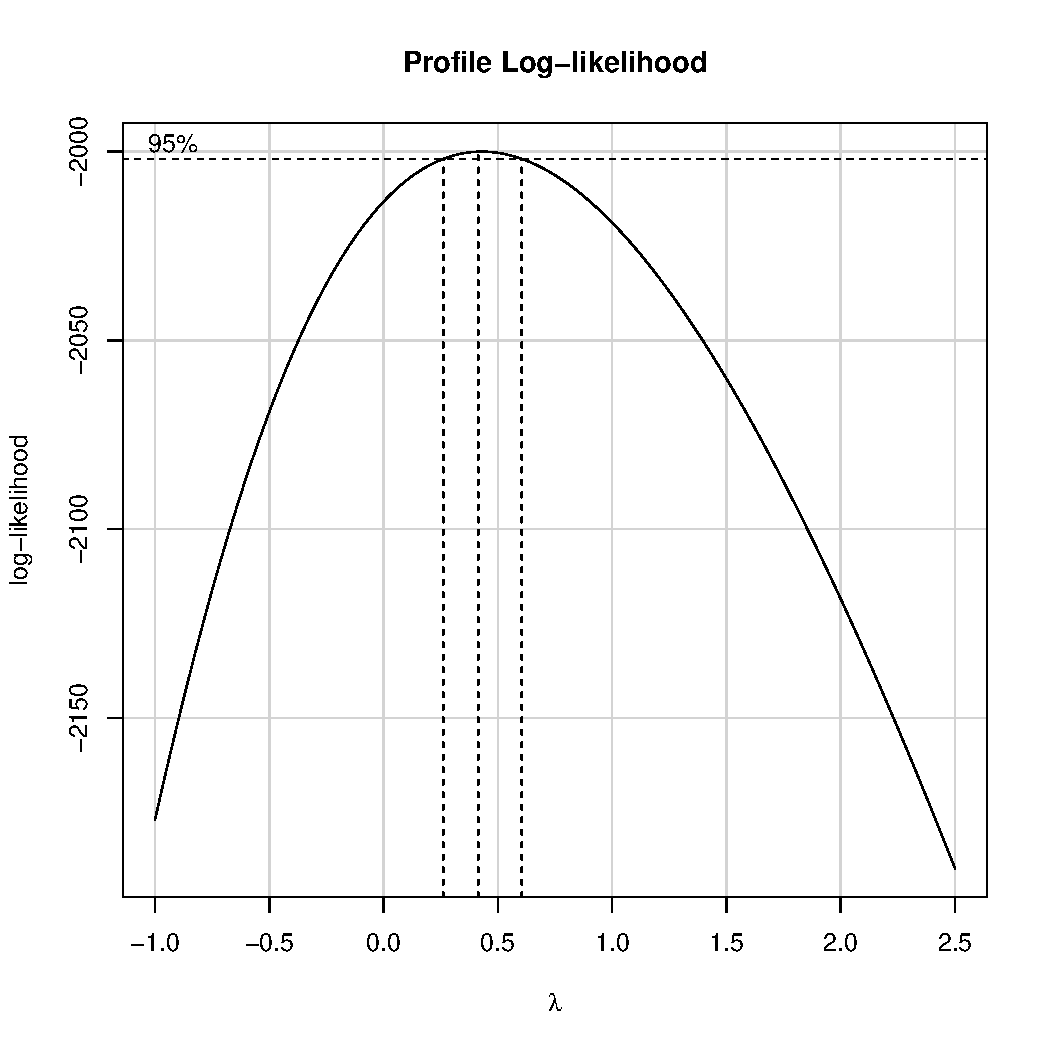
\includegraphics[scale = 0.5, keepaspectratio=true]{../Figures/plot_like_car}
  \caption{Log-likelihood Function for Box-Cox Transformation (\texttt{car} package)} \label{fig:plot_like_car}
\end{figure}


\clearpage
\section*{Using the \texttt{EnvStats} Package}


The \texttt{EnvStats} package is another option
but it is one designed for environmental statistics.
That is, it is not a generic package designed for the population of statisticians at large.
For that reason, it is missing some of the features that
a statistician would expect.
The notation and interpretation, however, are similar, 
except that the straight call to \texttt{boxcox}
simply does the calculation, 
unless you specify otherwise.

\begin{lstlisting}[language=R]
> # Find optimal value of lambda.
> bc_grid_ES_opt <- EnvStats::boxcox(x = flyreels[, 'Price'],
+                                    lambda = range(lambda_grid),
+                                    optimize = TRUE,
+                                    objective.name = "Log-Likelihood")
> 
> bc_grid_ES_opt$lambda
[1] 0.4295551
> 
\end{lstlisting}


The output is plotted in Figure \ref{fig:plot_like_EnvStats}.

\begin{figure}[h!]
  \centering
  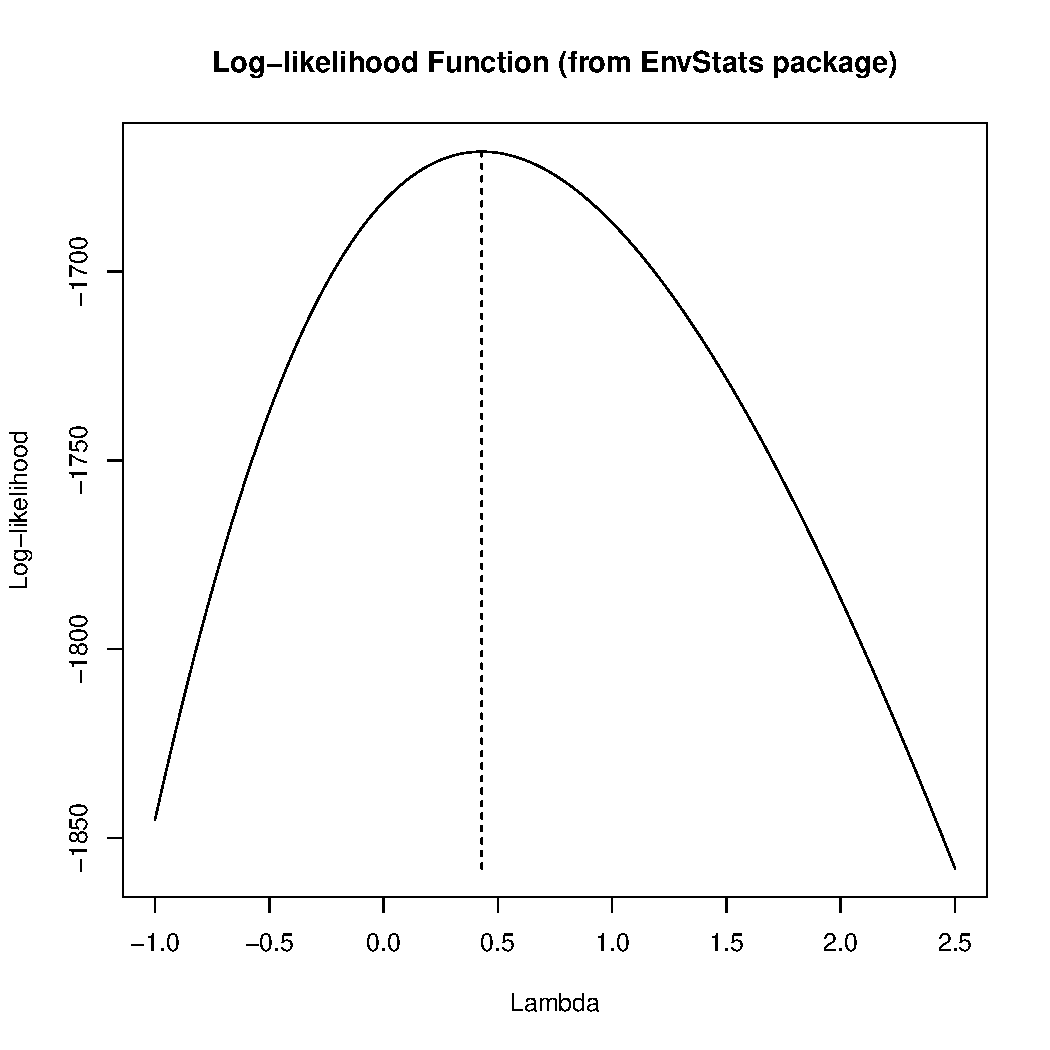
\includegraphics[scale = 0.5, keepaspectratio=true]{../Figures/plot_like_EnvStats}
  \caption{Log-likelihood Function for Box-Cox Transformation (\texttt{EnvStats} package)} \label{fig:plot_like_EnvStats}
\end{figure}






\clearpage
\section*{Normality of the Transformed Variable}

Now compare the quantiles of the distribution of the transformed variable with 
the original. 
We already plotted normal QQ plot for fly reel prices when considering the log transformation.
Now we can generate a new dependent variable with the results from the estimates above.


\begin{lstlisting}[language=R]
# Generate new dependent variable with results from estimates above.
flyreels[, 'Trans_Price'] <- Lambda_Price(price = flyreels[, 'Price'],
                                          lambda = lambda_hat)
\end{lstlisting}

Figure \ref{fig:qq_prices} shows this comparison
and the panel on the right, Figure \ref{subfig:qq_boxcox}, 
shows that the quantiles of the distribution of the transformed variable
nearly overlap with those of the normal distribution.
From a purely statistical perspective, 
this provides evidence that the prices are best modeled with the transformation
at the optimal $\lambda = 0.43$.
From a practical point of view, however, 
it is still an open question whether this 
added complexity is warranted when other variables are added to the model. 


\begin{figure}[!ht]
\subfloat[Fly Reel Prices\label{subfig:qq_prices}]{%
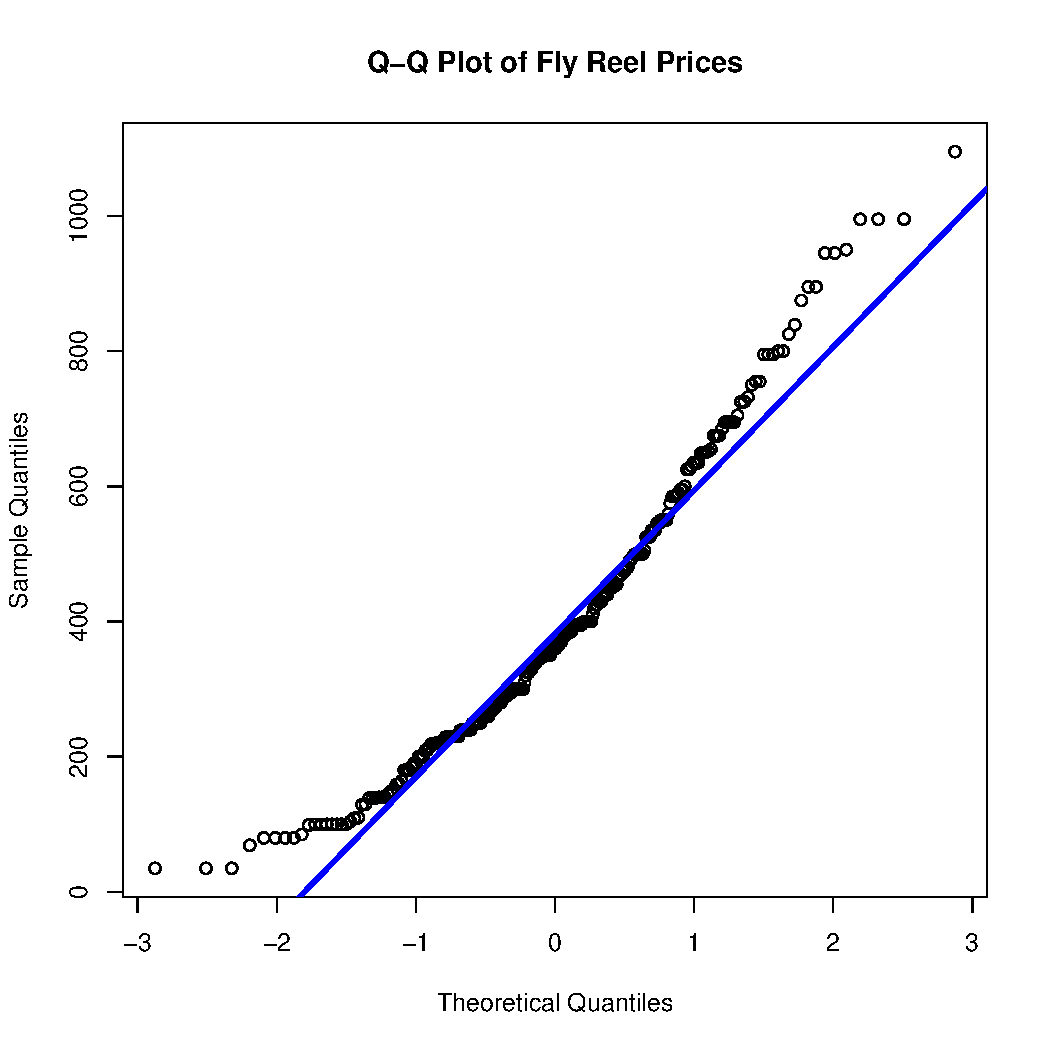
\includegraphics[width=0.5\textwidth]{../Figures/qq_prices}}
\hfill
\subfloat[Transformed Fly Reel Prices\label{subfig:qq_boxcox}]{%
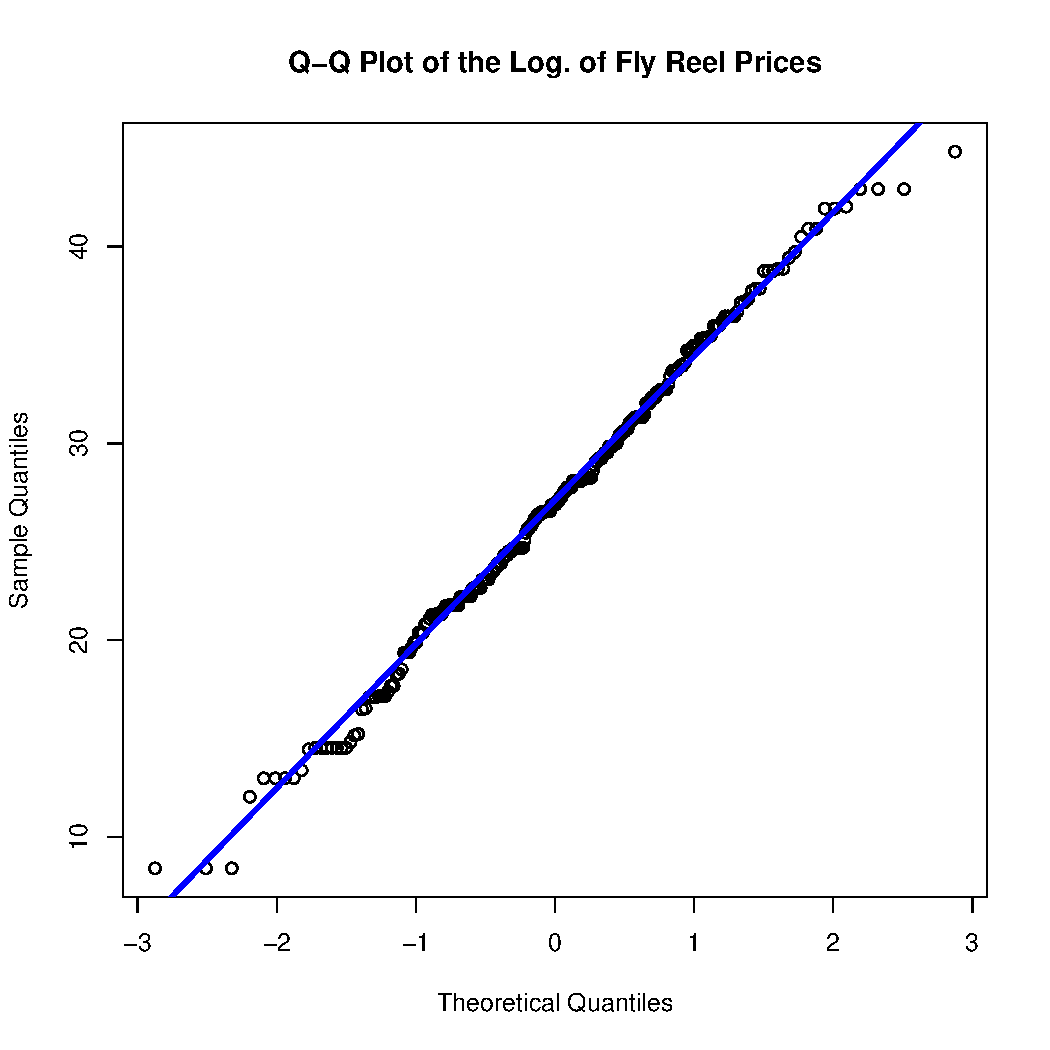
\includegraphics[width=0.5\textwidth]{../Figures/qq_boxcox}}

\caption{Q-QPlots of the Transformed Fly Reel Prices}
\label{fig:qq_prices}
\end{figure}








%%%%%%%%%%%%%%%%%%%%%%%%%%%%%%%%%%%%%%%%
\end{document}
%%%%%%%%%%%%%%%%%%%%%%%%%%%%%%%%%%%%%%%%


\pagebreak
\chapter{Preliminary Tabular Analysis}
%%%%%%%%%%%%%%%%%%%%%%%%%%%%%%%%%%%%%%%%%%%%%%%%%%%%%%%%%%%%
%
%\documentclass[11pt]{article}
%\usepackage{fullpage}
%\begin{document}
%
%
%%%%%%%%%%%%%%%%%%%%%%%%%%%%%%%%%%%%%%%%%%%%%%%%%%%%%%%%%%%%%
%
%{\noindent\bf Spring 2021 \hfill First Last}
%\vskip 16pt
%\centerline{\bf University of Central Florida}
%\centerline{\bf College of Business }
%\vskip 16pt
%\centerline{\bf QMB 6912}
%\centerline{\bf Capstone Project in Business Analytics}
%\vskip 10pt
%\centerline{\bf Problem Set \#3}
%\vskip 32pt
%\noindent
%% 
%\section{Data Description}
%% 
%By engaging an industry consultant to gather relevant and appropriate 
%information, your firm has been able to put together data concerning 248 
%different fly-fishing reels, over one-half of which are produced in the 
%United States, with the remainder being produced in Asia---either in China 
%or Korea.  These data are contained in the file {\tt FlyReels.csv}, which is
%available in the {\tt Data} folder.
%Each fly-fishing reel in the data set is a row, while the columns correspond 
%to the variables whose names and definitions are the following:
%\bigskip
%\begin{table}[ht]
%\centering
%\begin{tabular}{ll}
%  \hline
%    Variable & Definition \\
%  \hline
%
%    {\tt Name}        &product name (a string) \\ 
%    {\tt Brand}       &brand name (a string) \\ 
%    {\tt Weight}      &weight of reel in ounces (a real number) \\ 
%    {\tt Diameter}    &diameter of reel in inches (a real number) \\ 
%    {\tt Width}       &width of reel in inches (a real number) \\ 
%    {\tt Price}       &price of reel in dollars (a real number) \\ 
%    {\tt Sealed}      &whether the reel is sealed; {\tt "Yes"} versus
%                        {\tt "No"} (a string) \\ 
%    {\tt Country}     &country of manufacture, (a string) \\ 
%    {\tt Machined}    &whether the reel is machined versus cast;
%                        machined={\tt "Yes"}, \\ 
%                      &while cast={\tt "No"} (a string) \\ 
%  \hline
%\end{tabular}
%%\caption{Summary of Numeric Variables}
%%\label{tab:summary}
%\end{table}
%
%\bigskip
%\noindent
%I have downloaded the file {\tt FlyReels.csv}, 
%loaded the data described above into 
%\textsf{R}, 
%calculated the summary statistics for these data, 
%and finally, presented 
%these statistics in \LaTeX\ tables.
%These operations are all performed by the script 
%{\tt FlyReel\_Tables.R} in the {\tt Code} folder. 
%The script uses an \textsf{R} package called {\tt xtable} 
%to automate the
%production of the tables from a data frames in \textsf{R}.)
%
%\medskip
%\noindent

I analyze the data in subsets, according to country of manufacture, 
calculating the summary statistics for each subset and present these 
statistics in the \LaTeX\ tables that follow.

\vfill

%%%%%%%%%%%%%%%%%%%%%%%%%%%%%%%%%%%%%%%%%%%%%%%%%%%%%%%%%%%%

\pagebreak
\section{Summary by Country of Manufacture}

Table \ref{tab:summ_by_country} lists summary statistics for numeric variables
in separate columns for subsamples defined by the country of manufacture. 

% latex table generated in R 4.0.5 by xtable 1.8-4 package
% Thu Jan 27 21:16:18 2022
\begin{table}[ht]
\centering
\begin{tabular}{rlll}
  \hline
 & China & Korea & USA \\ 
  \hline
Min. Weight &  3.000 &  7.296 & 12.900 \\ 
  Mean Weight &  2.100 &  6.500 & 15.097 \\ 
  Max. Weight &  2.540 &  6.459 & 14.800 \\ 
  Min. Diameter & 2.500 & 3.935 & 5.250 \\ 
  Mean Diameter & 2.750 & 3.925 & 5.500 \\ 
  Max. Diameter & 2.700 & 3.878 & 5.430 \\ 
  Min. Width & 0.790 & 1.093 & 1.570 \\ 
  Mean Width & 0.7874 & 1.1434 & 1.5800 \\ 
  Max. Width & 0.750 & 1.070 & 1.688 \\ 
  Min. Price & 129.0 & 331.6 & 600.0 \\ 
  Mean Price &  34.99 & 280.22 & 839.00 \\ 
  Max. Price &  200.0 &  484.9 & 1095.0 \\ 
   \hline
\end{tabular}
\caption{Summary by Country of Manufacture} 
\label{tab:summ_by_country}
\end{table}



\pagebreak
\section{Country of Manufacture by Brand of Fly Reel}

Table \ref{tab:country_by_brand} lists the frequencies of observations of 
each brand of fly reel by country of manufacture. 

% latex table generated in R 4.0.5 by xtable 1.8-4 package
% Thu Jan 27 21:16:18 2022
\begin{table}[ht]
\centering
\begin{tabular}{rrrrr}
  \hline
 & China & Korea & USA & Total \\ 
  \hline
3-TAND & 15 & 0 & 0 & 15 \\ 
  Abel & 0 & 0 & 15 & 15 \\ 
  Allen & 0 & 18 & 7 & 25 \\ 
  Aspen & 0 & 0 & 8 & 8 \\ 
  Bauer & 0 & 0 & 2 & 2 \\ 
  Cheeky & 11 & 0 & 0 & 11 \\ 
  ECHO & 0 & 12 & 0 & 12 \\ 
  Galvan & 0 & 0 & 23 & 23 \\ 
  Hatch & 0 & 0 & 8 & 8 \\ 
  Loop & 0 & 14 & 0 & 14 \\ 
  Nautilus & 0 & 0 & 15 & 15 \\ 
  Orvis & 1 & 0 & 1 & 2 \\ 
  Ross & 0 & 0 & 28 & 28 \\ 
  Sage & 0 & 6 & 0 & 6 \\ 
  Taylor & 0 & 12 & 0 & 12 \\ 
  TFO & 0 & 16 & 0 & 16 \\ 
  Tibor & 0 & 0 & 4 & 4 \\ 
  Waterworks-Lamson & 0 & 8 & 24 & 32 \\ 
  Totals & 27 & 86 & 135 & 248 \\ 
   \hline
\end{tabular}
\caption{Country of Manufacture by Brand of Fly Reel} 
\label{tab:country_by_brand}
\end{table}


\pagebreak
\section{Reel Design by Brand of Fly Reel}

Table \ref{tab:design_by_brand} lists the frequencies of observations of 
each brand of fly reel across two categorical variables:
whether the reel is sealed
and whether the reel is machined versus cast. 


% latex table generated in R 4.1.1 by xtable 1.8-4 package
% Sun Apr 10 13:32:52 2022
\begin{table}[ht]
\centering
\begin{tabular}{rrrrrr}
  \hline
 & Unsealed & Sealed & Cast & Machined & Total \\ 
  \hline
3-TAND & 0 & 15 & 0 & 15 & 15 \\ 
  Abel & 9 & 6 & 0 & 15 & 15 \\ 
  Allen & 8 & 17 & 1 & 24 & 25 \\ 
  Aspen & 8 & 0 & 0 & 8 & 8 \\ 
  Bauer & 0 & 2 & 0 & 2 & 2 \\ 
  Cheeky & 6 & 5 & 6 & 5 & 11 \\ 
  ECHO & 9 & 3 & 12 & 0 & 12 \\ 
  Galvan & 20 & 3 & 0 & 23 & 23 \\ 
  Hatch & 0 & 8 & 0 & 8 & 8 \\ 
  Loop & 0 & 14 & 0 & 14 & 14 \\ 
  Nautilus & 4 & 11 & 0 & 15 & 15 \\ 
  Orvis & 0 & 2 & 0 & 2 & 2 \\ 
  Ross & 21 & 7 & 0 & 28 & 28 \\ 
  Sage & 2 & 4 & 0 & 6 & 6 \\ 
  Taylor & 0 & 12 & 0 & 12 & 12 \\ 
  TFO & 4 & 12 & 4 & 12 & 16 \\ 
  Tibor & 3 & 1 & 0 & 4 & 4 \\ 
  Waterworks-Lamson & 0 & 32 & 8 & 24 & 32 \\ 
  Totals & 94 & 154 & 31 & 217 & 248 \\ 
   \hline
\end{tabular}
\caption{Reel Design by Brand of Fly Reel} 
\label{tab:design_by_brand}
\end{table}



%%%%%%%%%%%%%%%%%%%%%%%%%%%%%%%%%%%%%%%%%%%%%%%%%%%%%%%%%%%%

% \end{document}

%%%%%%%%%%%%%%%%%%%%%%%%%%%%%%%%%%%%%%%%%%%%%%%%%%%%%%%%%%%%


\pagebreak
\chapter{Preliminary Graphical Analysis}
\documentclass[11pt]{book}
\usepackage{palatino}
\usepackage{amsfonts,amsmath,amssymb}
% \usepackage{graphicx}


\ifx\pdftexversion\undefined
    \usepackage[dvips]{graphicx}
\else
    \usepackage[pdftex]{graphicx}
    \usepackage{epstopdf}
    \epstopdfsetup{suffix=}
\fi


\begin{document}

%%%%%%%%%%%%%%%%%%%%%%%%%%%%%%%%%%%%%%%%
% Problem Set 5
%%%%%%%%%%%%%%%%%%%%%%%%%%%%%%%%%%%%%%%%

\pagestyle{empty}
{\noindent\bf Spring 2023 \hfill Firstname M.~Lastname}
\vskip 16pt
\centerline{\bf University of Central Florida}
\centerline{\bf College of Business}
\vskip 16pt
\centerline{\bf QMB 6911}
\centerline{\bf Capstone Project in Business Analytics}
\vskip 10pt
\centerline{\bf Solutions:  Problem Set \#5}
\vskip 32pt
\noindent




\section{Histogram and Density of Log. Fly Reel Prices}

To begin visually analyzing the data, 
include plots of the density that were created last week.

\subsection{All Fly Reels Together}

Start with the log of prices because prices were skewed.
Figure \ref{fig:hist_dens_log_price} is
a histogram of the logarithm of fly reel prices, 
along with a rug plot and a kernel density estimate. 
%
\begin{figure}[h!]
  \centering
  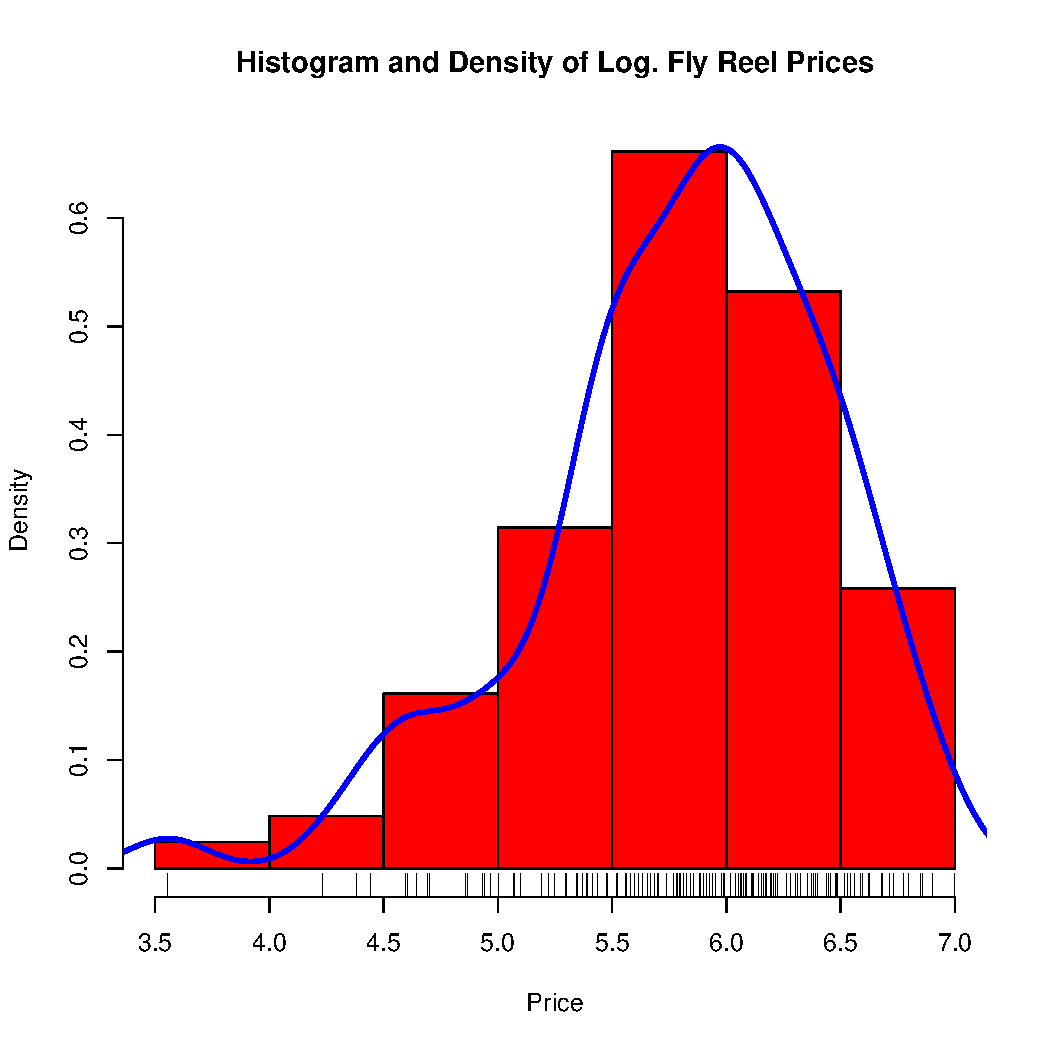
\includegraphics[scale = 0.5, keepaspectratio=true]{../Figures/hist_dens_log_price}
  \caption{Relative Histogram of Fly Reel Prices} \label{fig:hist_dens_log_price}
\end{figure}
% 
After taking logs, we can see that the distribution is
approximately symmetric, now with a slight skew to the left. 
Unlike the case of the tractors, 
the improvement from the log transformation is not so clear, 
so we should investigate this further in a later problem set. 


\clearpage
\pagebreak
\subsection{Comparison By Country of Manufacture}

Now we investigate the prices of fly reels made in the USA
compared to those made in China and Korea.
Figure \ref{fig:dens_by_country} shows the 
kernel density estimate of the prices of 
fly reels made in the USA in blue,
those made in China in red, 
and those made in Korea in green.
% 
The modes of the distributions are similar, 
however, we observe more variability in the prices of fly reels
made in Korea. 
The distribution of fly reels made in the USA is shifted 
toward the higher price range, compared to those made in other countries.
This indicates mild support for a ``Made in America'' premium
but we should also consider that it may be explained by 
the features of the reels made in the USA. 
We will investigate this further in regression analysis 
and other modeling approaches. 



\begin{figure}[h!]
  \centering
  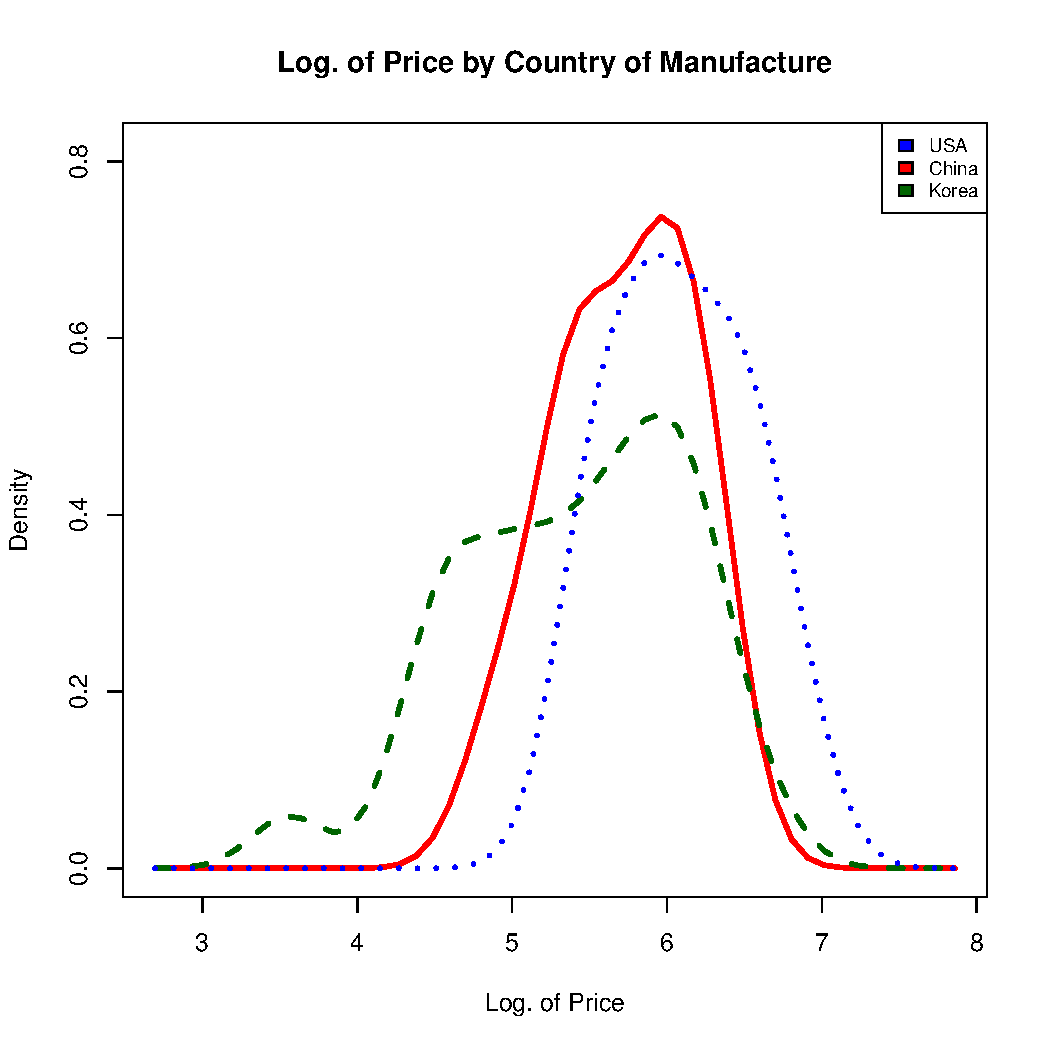
\includegraphics[scale = 0.5, keepaspectratio=true]{../Figures/dens_by_country}
  \caption{Densities of Log. Fly Reel Prices by Country of Manufacture} \label{fig:dens_by_country}
\end{figure}


\clearpage
\pagebreak
\section*{Scatterplot Matrices}


\subsection*{Scatterplots of Numeric Variables}

Figure \ref{fig:slpom_num_only} depicts a matrix of scatterplots
of the numeric variables in the dataset.

\begin{figure}[h!]
  \centering
  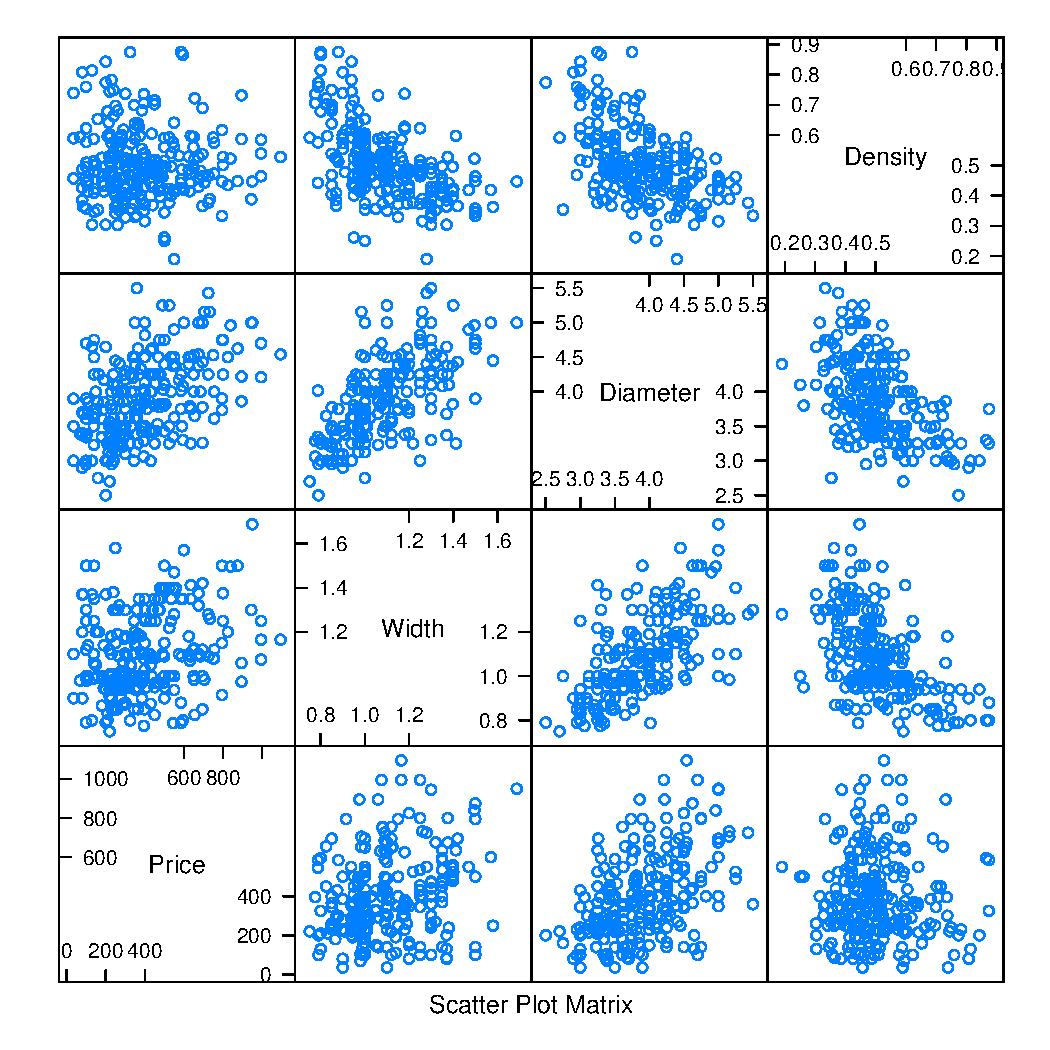
\includegraphics[scale = 0.5, keepaspectratio=true]{../Figures/slpom_num_only}
  \caption{Scatterplots of Numeric Variables} \label{fig:slpom_num_only}
\end{figure}


\pagebreak
\subsection*{Scatterplots with Categorical Variables}

Figure \ref{fig:slpom_with_cat} depicts a matrix of scatterplots
of with categorical variables in the dataset.

\begin{figure}[h!]
  \centering
  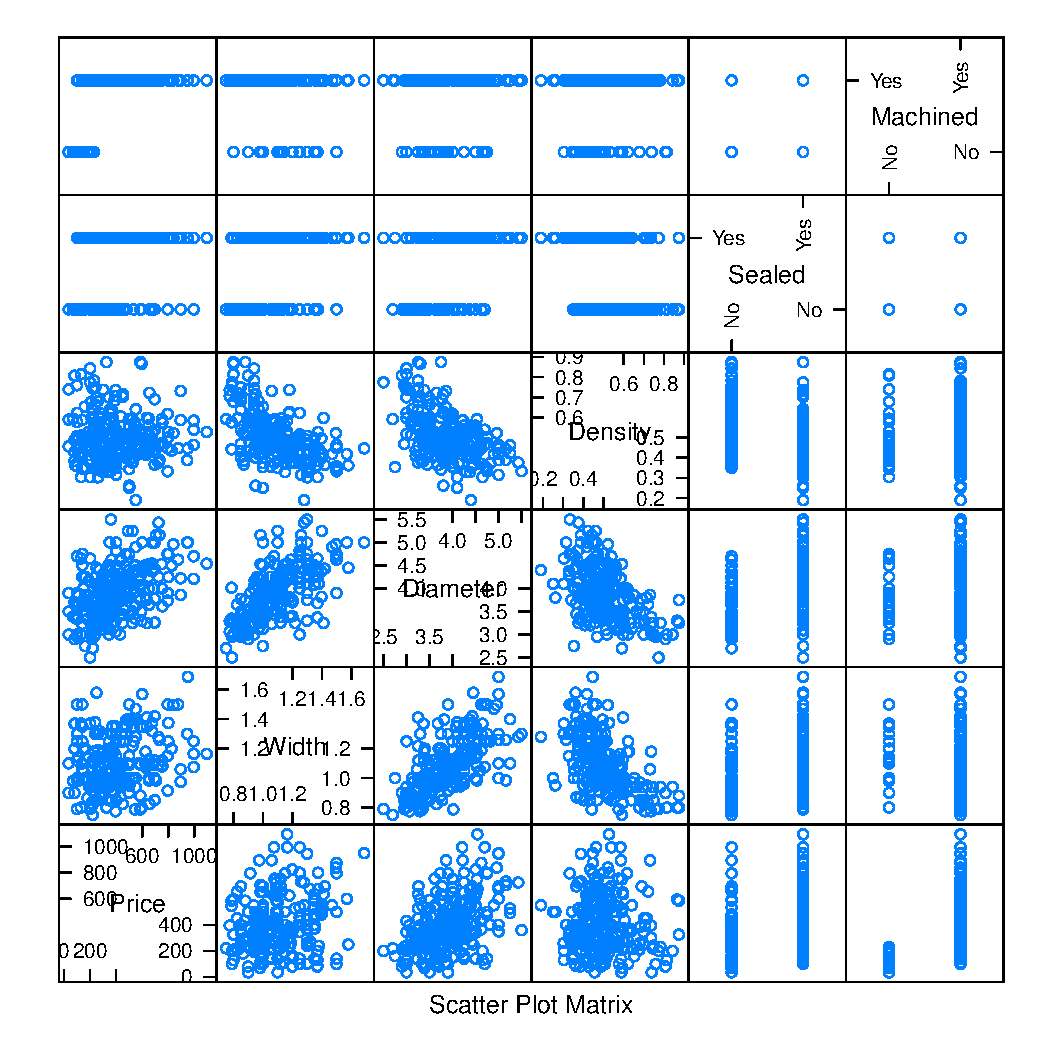
\includegraphics[scale = 0.5, keepaspectratio=true]{../Figures/slpom_with_cat}
  \caption{Scatterplots with Categorical Variables} \label{fig:slpom_with_cat}
\end{figure}


\pagebreak


Figure \ref{fig:slpom_with_sealed_mach.eps} depicts a matrix of scatterplots
with a categorical variable for the design combinations of the fly reels:
a fly reel is either sealed or unsealed and either machined or cast.

\begin{figure}[h!]
  \centering
  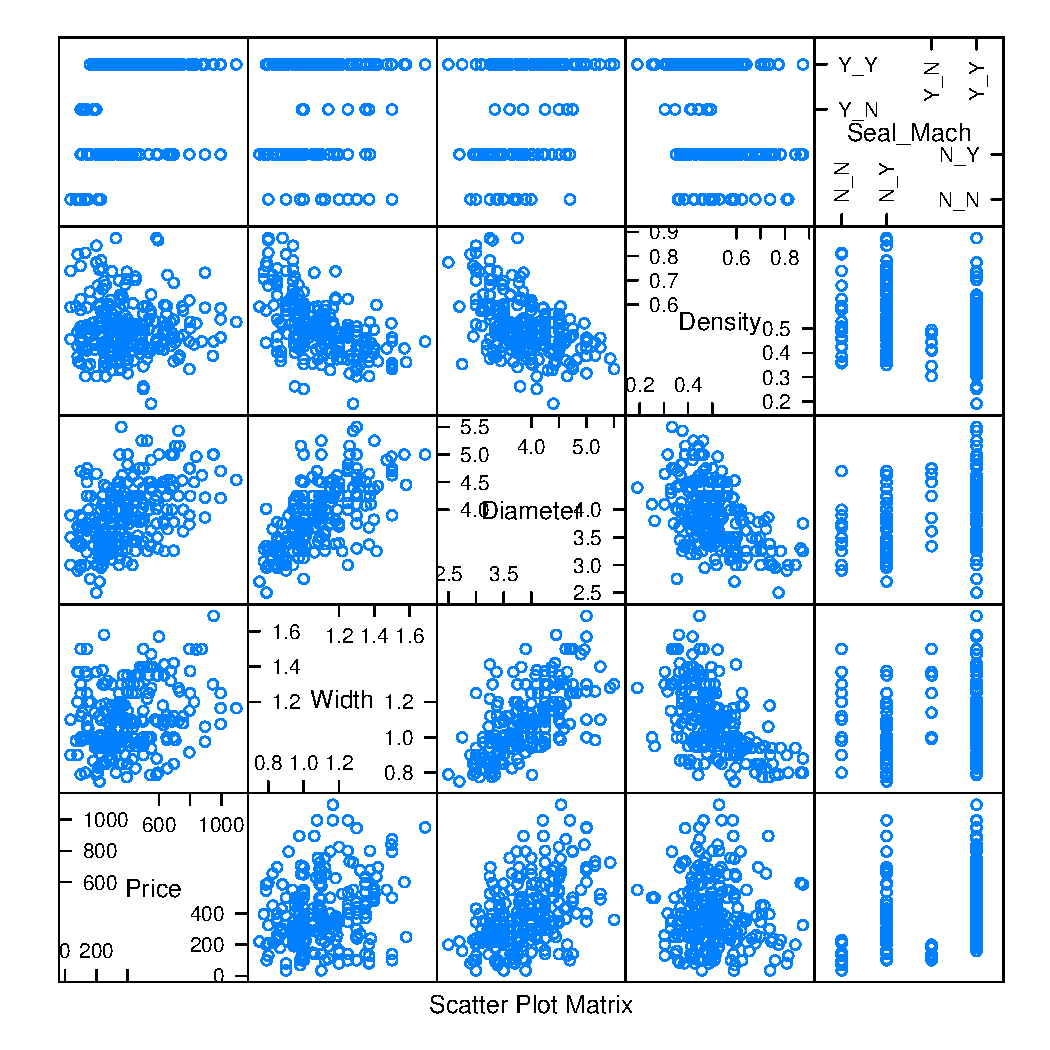
\includegraphics[scale = 0.5, keepaspectratio=true]{../Figures/slpom_with_sealed_mach.eps}
  \caption{Scatterplots of Numeric Variables} \label{fig:slpom_with_sealed_mach.eps}
\end{figure}



\pagebreak
\subsection*{Scatterplots by Country of Manufacture}

Figure \ref{fig:slpom_by_country} depicts a matrix of scatterplots
of the variables in the dataset
with the points indicated differently by country of manufacture.

\begin{figure}[h!]
  \centering
  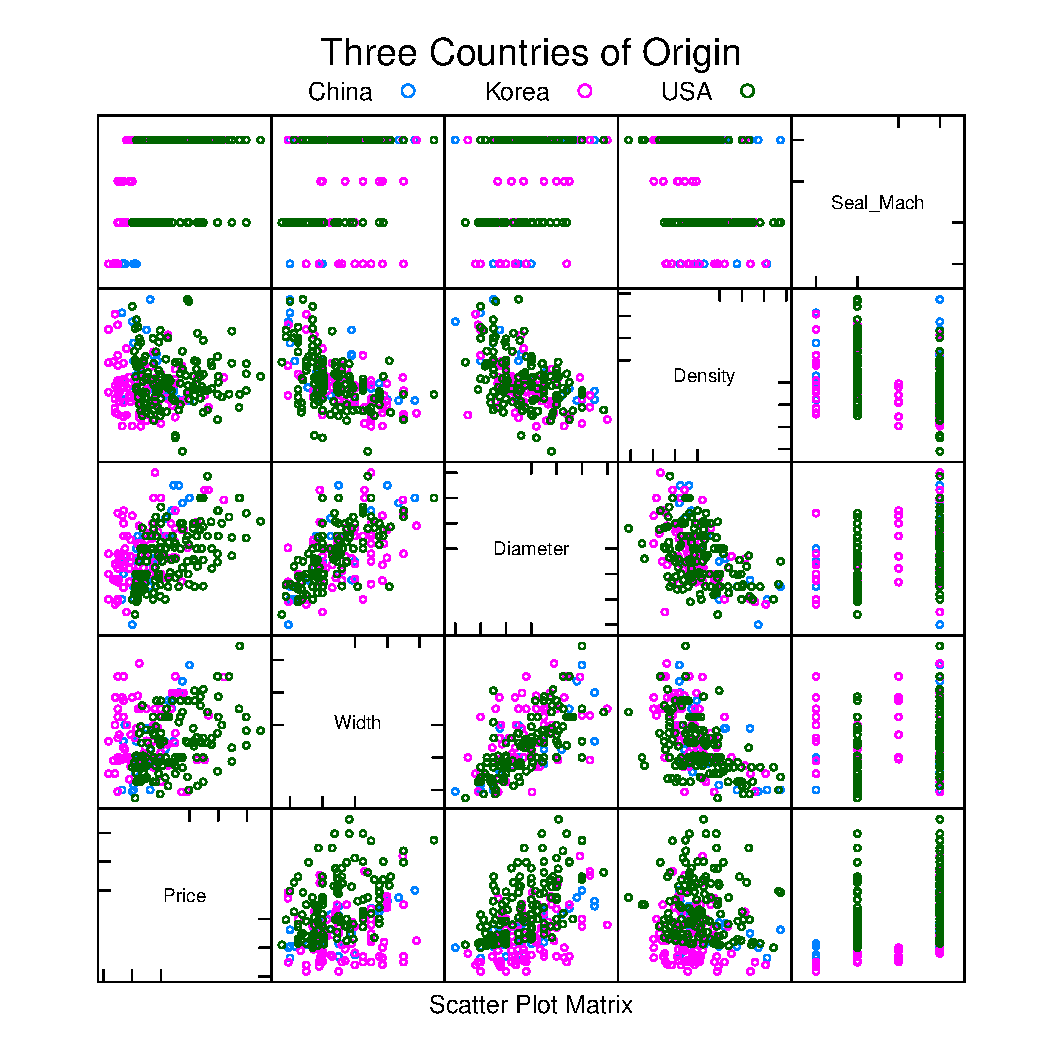
\includegraphics[scale = 0.5, keepaspectratio=true]{../Figures/slpom_by_country}
  \caption{Scatterplots by Country of Manufacture} \label{fig:slpom_by_country}
\end{figure}



\pagebreak
\subsection*{Dot Chart by Brand and Country of Manufacture}

Now consider the average prices by brand of fly reel and 
country of manufacture. 
Figure \ref{fig:dotchart_brand_country} depicts a dot chart
showing the average prices in the horizontal axis 
in these combinations of categories.


\begin{figure}[h!]
  \centering
  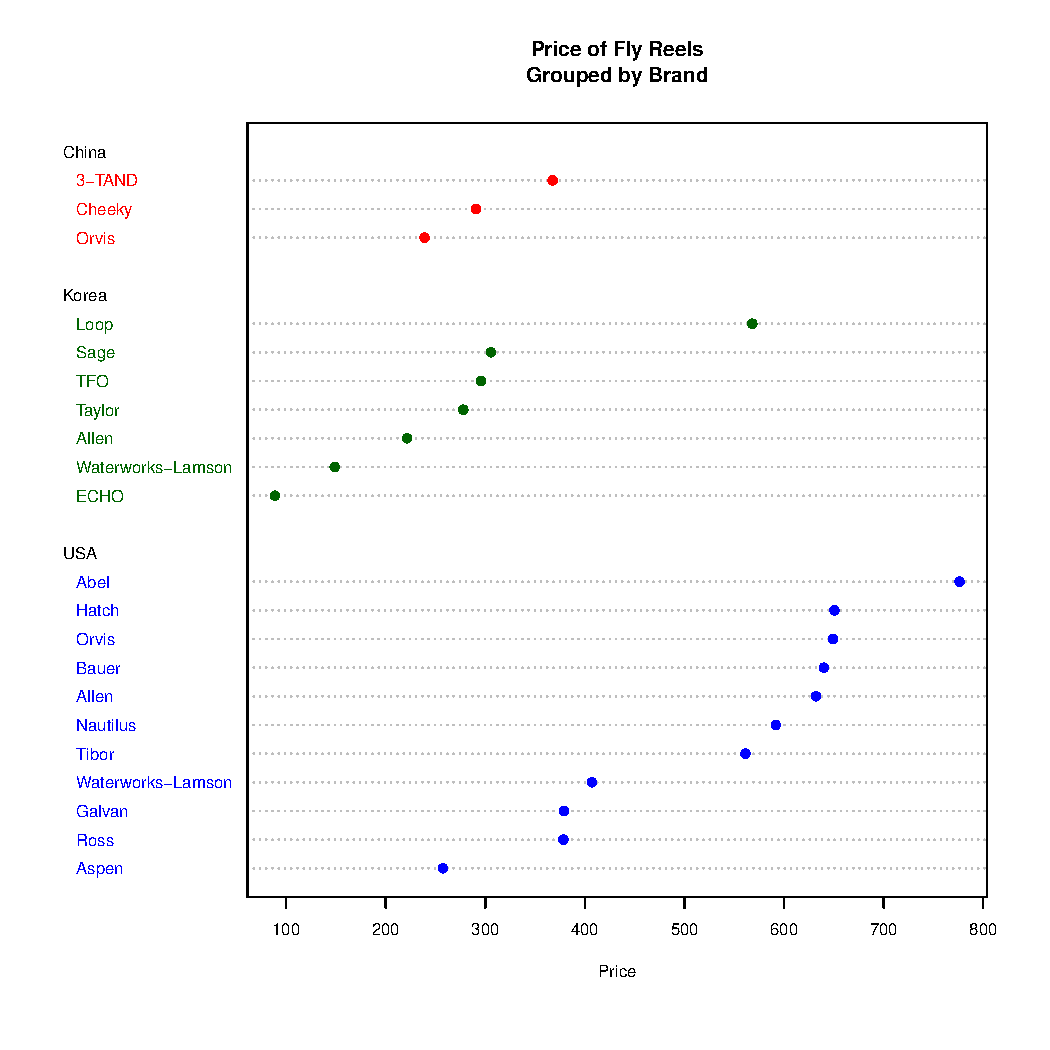
\includegraphics[scale = 0.5, keepaspectratio=true]{../Figures/dotchart_brand_country}
  \caption{Average Prices by Brand and Country of Manufacture} \label{fig:dotchart_brand_country}
\end{figure}

We see that there exists more variety, 
in terms of both the number of brands and price levels
within the population of American fly reel manufacturers. 
It's especially important that we consider the proliferation of 
fly reel brands at the high price points.
It is worth investigating further whether those fly reels
benefit from the ``Made in America'' premium
or are simply made with more valuable characteristics. 


%%%%%%%%%%%%%%%%%%%%%%%%%%%%%%%%%%%%%%%%
\end{document}
%%%%%%%%%%%%%%%%%%%%%%%%%%%%%%%%%%%%%%%%


\pagebreak
\chapter{Regression Modelling with Hedonic Price Theory}
%\documentclass[11pt]{paper}
%\usepackage{palatino}
%\usepackage{amsfonts,amsmath,amssymb}
%% \usepackage{graphicx}
%
%
%\usepackage{listings}
%\usepackage{textcomp}
%\usepackage{color}
%
%\definecolor{dkgreen}{rgb}{0,0.6,0}
%\definecolor{gray}{rgb}{0.5,0.5,0.5}
%\definecolor{mauve}{rgb}{0.58,0,0.82}
%
%\lstset{frame=tb,
%  language=R,
%  aboveskip=3mm,
%  belowskip=3mm,
%  showstringspaces=false,
%  columns=flexible,
%  basicstyle={\small\ttfamily},
%  numbers=none,
%  numberstyle=\tiny\color{gray},
%  keywordstyle=\color{blue},
%  commentstyle=\color{dkgreen},
%  stringstyle=\color{mauve},
%  breaklines=true,
%  breakatwhitespace=true,
%  tabsize=3
%}
%
%
%\ifx\pdftexversion\undefined
%    \usepackage[dvips]{graphicx}
%\else
%    \usepackage[pdftex]{graphicx}
%    % \usepackage{epstopdf}
%    % \epstopdfsetup{suffix=}
%    \usepackage[outdir=./]{epstopdf}
%\fi
%
%\usepackage{subfig}
%
%
%\begin{document}

%%%%%%%%%%%%%%%%%%%%%%%%%%%%%%%%%%%%%%%%
% Problem Set 7
%%%%%%%%%%%%%%%%%%%%%%%%%%%%%%%%%%%%%%%%

%\pagestyle{empty}
%{\noindent\bf Spring 2021 \hfill Firstname M.~Lastname}
%\vskip 16pt
%\centerline{\bf University of Central Florida}
%\centerline{\bf College of Business}
%\vskip 16pt
%\centerline{\bf QMB 6911}
%\centerline{\bf Capstone Project in Business Analytics}
%\vskip 10pt
%\centerline{\bf Solutions:  Problem Set \#7}
%\vskip 32pt
%\noindent


% \pagebreak
\section{Analyzing the Dependent Variable}

\subsection{Probability Density Function of Fly Reel Prices}

Figure \ref{fig:density_prices} is the kernel-smoothed probability density function of the natural logarithm of
price:

\begin{figure}[h!]
  \centering
  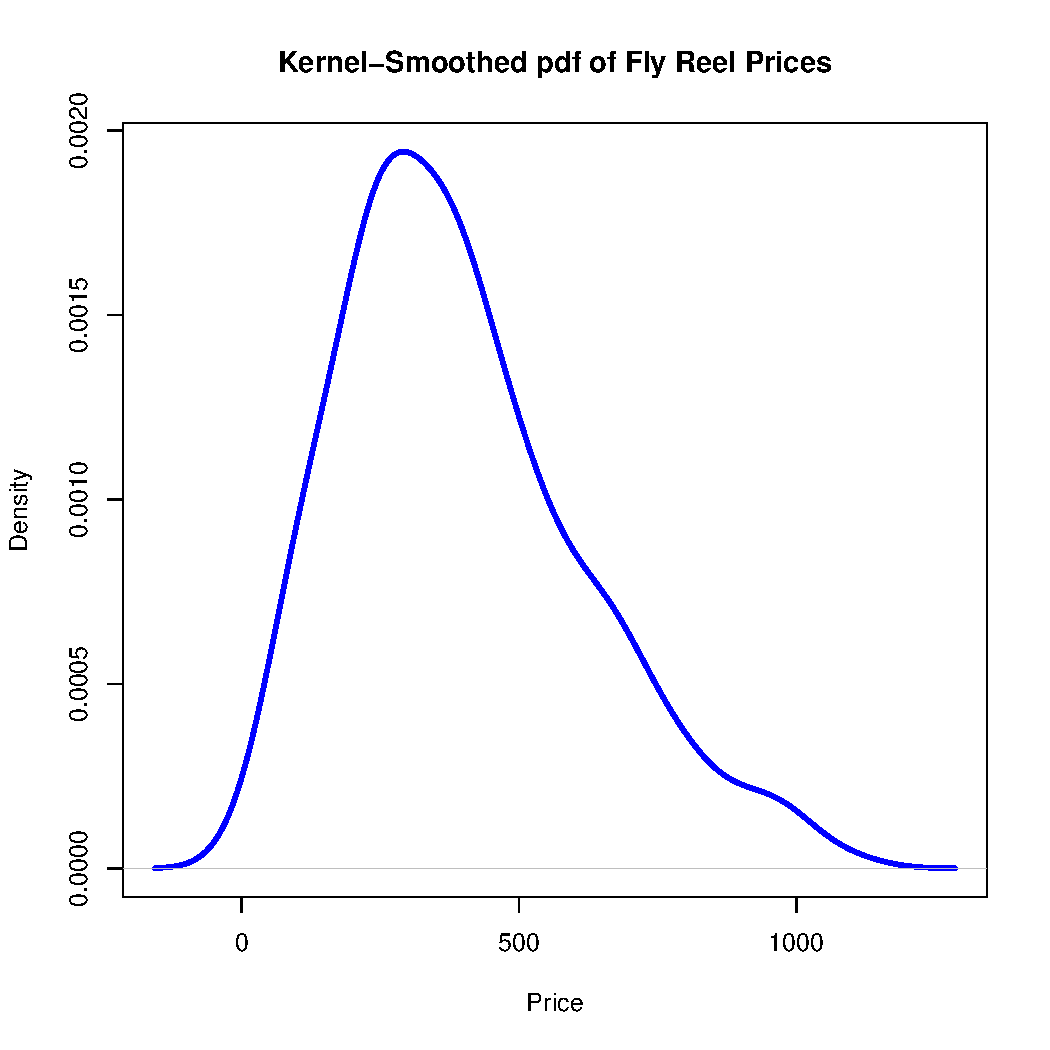
\includegraphics[scale = 0.5, keepaspectratio=true]{../Figures/density_prices}
  \caption{Probability Density Function of Fly Reel Prices} \label{fig:density_prices}
\end{figure}


\subsection{Probability Density Function of the Log. of Fly Reel Prices}

Figure \ref{fig:density_log_prices} is the kernel-smoothed probability density function of the natural logarithm of
price:

\begin{figure}[h!]
  \centering
  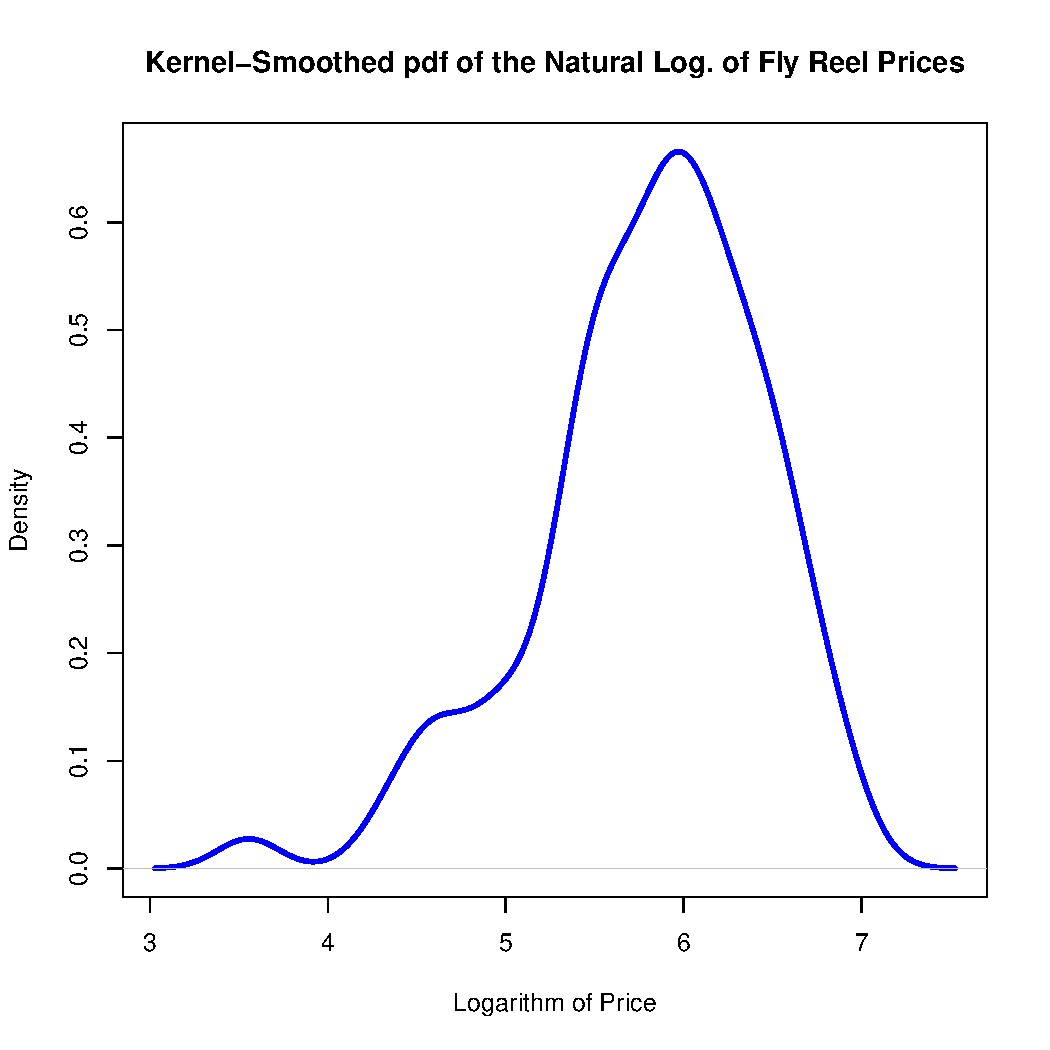
\includegraphics[scale = 0.5, keepaspectratio=true]{../Figures/density_log_prices}
  \caption{Probability Density Function of Fly Reel Prices} \label{fig:density_log_prices}
\end{figure}



\pagebreak
\subsection{Probability Density Function of the Box-Cox Transformation of Fly Reel Prices}

Figure \ref{fig:density_trans_prices} is the kernel-smoothed probability density function of the natural logarithm of
price. 
Although the transformed model does look closest to normal,
all three distributions are reasonably symmetric, 
indicating that the use of the transformation is subject to judgment.
Whether it is worth using the transformation
can be settled by analyzing the results of regression models 
with different forms of the dependent variable. 

\begin{figure}[h!]
  \centering
  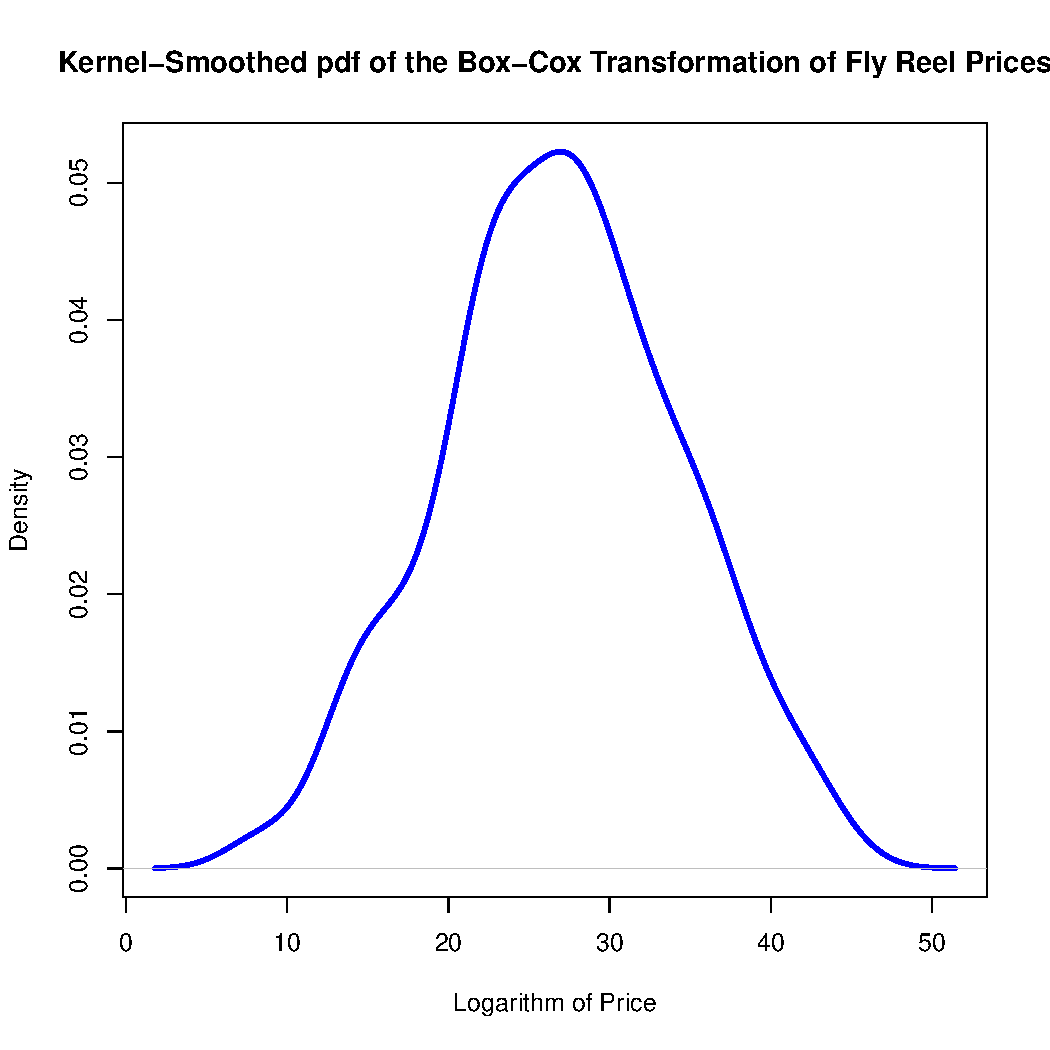
\includegraphics[scale = 0.5, keepaspectratio=true]{../Figures/density_trans_prices}
  \caption{Probability Density Function of Transformed Fly Reel Prices} \label{fig:density_trans_prices}
\end{figure}


\pagebreak
\section{Regression Models for Fly Reel Prices}


For the regression analysis, I create new variables.
The first is the volume of each reel, 
calculated as the volume of a cylinder: 
the value $\pi$ times the square of the radius of the reel,
times the width of the reel. 
The density is then calculated as the weight 
divided by the volume. 

\begin{lstlisting}[language=R]
R> flyreels[, 'Volume'] <- 
	pi * (flyreels[, 'Diameter']/2)^2 * flyreels[, 'Width']
R> flyreels[, 'Density'] <- 
	flyreels[, 'Weight'] / flyreels[, 'Volume']
\end{lstlisting}



% \pagebreak
\subsection{Comparison by Transformation of Dependent Variable}

Table \ref{tab:reg_by_dep_var} shows the results of 
a series of regression models with different definitions of the dependent variable.
Model 1 uses the fly reel prices without transformation, 
Model 2 uses the logarithm of the fly reel prices, 
and Model 3 uses the Box-Cox transformation of fly reel prices, 
with the optimal value of the parameter in the exponent.
% 
Although the model built on the original price levels
has statistically significant coefficients, 
the two transformed models have a better fit, 
with higher values of $\bar{R}^2$. 
Since the difference between the latter two models is marginal, 
it is better to model the logarithm of fly reel prices, 
which has the added advantage of interpretability 
of the coefficients, 
which approximately represent percentage changes in fly reel prices. 


\begin{table}
\begin{center}
\begin{tabular}{l c c c}
\hline
 & Model 1 & Model 2 & Model 3 \\
\hline
(Intercept)       & $-1056.01^{***}$ & $2.09^{***}$ & $-19.77^{***}$ \\
                  & $(105.51)$       & $(0.26)$     & $(3.21)$       \\
Width             & $158.71^{*}$     & $0.30$       & $4.38^{*}$     \\
                  & $(63.32)$        & $(0.16)$     & $(1.92)$       \\
Diameter          & $174.36^{***}$   & $0.40^{***}$ & $5.37^{***}$   \\
                  & $(20.59)$        & $(0.05)$     & $(0.63)$       \\
Density           & $596.81^{***}$   & $1.20^{***}$ & $17.19^{***}$  \\
                  & $(89.17)$        & $(0.22)$     & $(2.71)$       \\
SealedYes         & $144.31^{***}$   & $0.42^{***}$ & $5.00^{***}$   \\
                  & $(20.43)$        & $(0.05)$     & $(0.62)$       \\
MachinedYes       & $114.40^{***}$   & $0.76^{***}$ & $6.53^{***}$   \\
                  & $(30.43)$        & $(0.08)$     & $(0.92)$       \\
made\_in\_USATRUE & $202.10^{***}$   & $0.52^{***}$ & $6.51^{***}$   \\
                  & $(19.86)$        & $(0.05)$     & $(0.60)$       \\
\hline
R$^2$             & $0.64$           & $0.74$       & $0.71$         \\
Adj. R$^2$        & $0.63$           & $0.73$       & $0.70$         \\
Num. obs.         & $248$            & $248$        & $248$          \\
\hline
\multicolumn{4}{l}{\scriptsize{$^{***}p<0.001$; $^{**}p<0.01$; $^{*}p<0.05$}}
\end{tabular}
\caption{Regression Models with Different Dependent Variables}
\label{tab:reg_by_dep_var}
\end{center}
\end{table}


\pagebreak
\subsection{Comparison by Country of Manufacture}

Table \ref{tab:reg_by_country} shows the results of 
a series of regression models 
on different samples by country of manufacture.
Model 1 shows the results for the sample of fly reels made in the USA
and Model 2 shows the remaining fly reels made in China or Korea.


\begin{table}
\begin{center}
\begin{tabular}{l c c c c}
\hline
 & Model 1 & Model 2 & Model 3 & Model 4 \\
\hline
(Intercept) & $3.35^{***}$ & $3.48^{***}$ & $2.03^{***}$ & $2.41^{***}$ \\
            & $(0.30)$     & $(0.28)$     & $(0.47)$     & $(0.41)$     \\
Width       & $0.28$       &              & $0.39$       &              \\
            & $(0.22)$     &              & $(0.23)$     &              \\
Diameter    & $0.44^{***}$ & $0.49^{***}$ & $0.36^{***}$ & $0.41^{***}$ \\
            & $(0.07)$     & $(0.05)$     & $(0.08)$     & $(0.07)$     \\
Density     & $1.13^{***}$ & $1.06^{***}$ & $1.32^{**}$  & $1.06^{**}$  \\
            & $(0.25)$     & $(0.25)$     & $(0.41)$     & $(0.38)$     \\
SealedYes   & $0.32^{***}$ & $0.32^{***}$ & $0.65^{***}$ & $0.64^{***}$ \\
            & $(0.06)$     & $(0.06)$     & $(0.10)$     & $(0.10)$     \\
MachinedYes &              &              & $0.65^{***}$ & $0.63^{***}$ \\
            &              &              & $(0.09)$     & $(0.09)$     \\
\hline
R$^2$       & $0.54$       & $0.53$       & $0.75$       & $0.74$       \\
Adj. R$^2$  & $0.52$       & $0.52$       & $0.73$       & $0.73$       \\
Num. obs.   & $135$        & $135$        & $113$        & $113$        \\
\hline
\multicolumn{5}{l}{\scriptsize{$^{***}p<0.001$; $^{**}p<0.01$; $^{*}p<0.05$}}
\end{tabular}
\caption{Regression Models by Country of Manufacture}
\label{tab:reg_by_country}
\end{center}
\end{table}


The width of the reel is insignificant in both samples
and the coefficients are qualitatively similar across the samples, as well as matching in significance. 
This suggests that one model might be sufficient. 

To test this statistically, I conduct an $F$-test. 
This compares a single model with only an
indicator for the country of manufacture
(the restricted model)
with a separate model for each country.
In this case, the full, unrestricted model has 
$K = 2\times6 = 12$ parameters, one for each variable in two models. 
The test that all of the coefficients are the same has 
$M = 6 - 1 = 5$
restrictions. 
The one restriction fewer accounts for the made-in-USA indicator
in the full model, 
which allows for two separate intercepts. 
% 
The $F$-statistic has a value of 

$$ 
\frac{(RSS_M - RSS)/M}{RSS/(N - K - 1)} = \frac{(26.24962 - 25.2235)/5}{25.2235/235} = 1.912007. 
$$

This value is greater than 1, so we can compare it to the critical value
of the $F$-statistic at the specified degrees of freedom for
a conventional level of significance.
These critical values are 
3.095, 2.252, and 1.872
at the 1\%, 5\%, and 10\%
levels of significance, respectively.

This places the F-statistic between the critical values for the
5 and 10 percent levels of significance.
Conclude that fly reel prices may have some difference by
country of manufacture but the difference is marginal.
This suggests little justification for separate models by
country of manufacture.
We can investigate small differences between the models.


In the next section, 
I will consider a hybrid model with some interaction terms
with separate coefficients by country of manufacture. 


\pagebreak
\subsection{Models with Interaction Terms}

Table \ref{tab:reg_interactions} shows the results of 
a series of regression models with different 
specifications of interaction terms by country of manufacture. 
% 
The interaction with sealed and country of manufacture is significant in both specifications Model 1 and Model 3.
In contrast, the interaction with density was not significant. 
Furthermore, the width of fly reels is a significant predictor
in this more refined model. 
Since all variables are significant in this model and it
has the highest $\bar{R}^2$, Model 1 is the recommended model.



\begin{table}
\begin{center}
\begin{tabular}{l c c c c}
\hline
 & Model 1 & Model 2 & Model 3 & Model 4 \\
\hline
(Intercept)          & $8.89189^{***}$  & $8.88028^{***}$  & $8.87926^{***}$  & $8.89127^{***}$  \\
                     & $(0.12827)$      & $(0.11042)$      & $(0.11163)$      & $(0.11165)$      \\
horsepower           & $0.00488^{***}$  & $0.00490^{***}$  & $0.00489^{***}$  & $0.00476^{***}$  \\
                     & $(0.00039)$      & $(0.00039)$      & $(0.00039)$      & $(0.00043)$      \\
age                  & $-0.02986^{***}$ & $-0.02994^{***}$ & $-0.02990^{***}$ & $-0.02969^{***}$ \\
                     & $(0.00381)$      & $(0.00381)$      & $(0.00400)$      & $(0.00381)$      \\
enghours             & $-0.00004$       & $-0.00004^{***}$ & $-0.00004^{***}$ & $-0.00004^{***}$ \\
                     & $(0.00003)$      & $(0.00001)$      & $(0.00001)$      & $(0.00001)$      \\
diesel               & $0.28447^{*}$    & $0.30271^{**}$   & $0.29874^{**}$   & $0.29293^{**}$   \\
                     & $(0.12619)$      & $(0.10378)$      & $(0.10389)$      & $(0.10387)$      \\
fwd                  & $0.25952^{***}$  & $0.25727^{***}$  & $0.25879^{***}$  & $0.26050^{***}$  \\
                     & $(0.06238)$      & $(0.06230)$      & $(0.06229)$      & $(0.06226)$      \\
manual               & $-0.16119^{*}$   & $-0.15793^{*}$   & $-0.16018^{*}$   & $-0.16217^{*}$   \\
                     & $(0.06631)$      & $(0.06632)$      & $(0.06692)$      & $(0.06619)$      \\
johndeere            & $0.31091^{***}$  & $0.25824^{*}$    & $0.30345^{*}$    & $0.24957^{*}$    \\
                     & $(0.07868)$      & $(0.11399)$      & $(0.15228)$      & $(0.10998)$      \\
cab                  & $0.67506^{***}$  & $0.67717^{***}$  & $0.67571^{***}$  & $0.67665^{***}$  \\
                     & $(0.06732)$      & $(0.06728)$      & $(0.06734)$      & $(0.06722)$      \\
enghours:diesel      & $0.00001$        &                  &                  &                  \\
                     & $(0.00003)$      &                  &                  &                  \\
enghours:johndeere   &                  & $0.00001$        &                  &                  \\
                     &                  & $(0.00002)$      &                  &                  \\
age:johndeere        &                  &                  & $0.00023$        &                  \\
                     &                  &                  & $(0.00742)$      &                  \\
horsepower:johndeere &                  &                  &                  & $0.00057$        \\
                     &                  &                  &                  & $(0.00077)$      \\
\hline
R$^2$                & $0.77769$        & $0.77795$        & $0.77766$        & $0.77811$        \\
Adj. R$^2$           & $0.77017$        & $0.77043$        & $0.77014$        & $0.77060$        \\
Num. obs.            & $276$            & $276$            & $276$            & $276$            \\
\hline
\multicolumn{5}{l}{\scriptsize{$^{***}p<0.001$; $^{**}p<0.01$; $^{*}p<0.05$}}
\end{tabular}
\caption{Regression Models for Tractor Prices}
\label{tab:reg_interactions}
\end{center}
\end{table}



In terms of the production decision, 
there exists a substantial premium for fly reels made in the USA
but this premium is half as large for sealed reels, 
however, this reduced premium is still smaller than the 
additional value for a sealed reel.  


%%%%%%%%%%%%%%%%%%%%%%%%%%%%%%%%%%%%%%%%
% \end{document}
%%%%%%%%%%%%%%%%%%%%%%%%%%%%%%%%%%%%%%%%


\pagebreak
\chapter{Nonparametric Regression Models}
\documentclass[11pt]{paper}
\usepackage{fullpage}
\usepackage{palatino}
\usepackage{amsfonts,amsmath,amssymb}
% \usepackage{graphicx}

\usepackage{listings}
\usepackage{textcomp}
\usepackage{color}

\definecolor{dkgreen}{rgb}{0,0.6,0}
\definecolor{gray}{rgb}{0.5,0.5,0.5}
\definecolor{mauve}{rgb}{0.58,0,0.82}

\lstset{frame=tb,
  language=R,
  aboveskip=3mm,
  belowskip=3mm,
  showstringspaces=false,
  columns=flexible,
  basicstyle={\small\ttfamily},
  numbers=none,
  numberstyle=\tiny\color{gray},
  keywordstyle=\color{blue},
  commentstyle=\color{dkgreen},
  stringstyle=\color{mauve},
  breaklines=true,
  breakatwhitespace=true,
  tabsize=3
}



\ifx\pdftexversion\undefined
    \usepackage[dvips]{graphicx}
\else
    \usepackage[pdftex]{graphicx}
    \usepackage{epstopdf}
    \epstopdfsetup{suffix=}
\fi

\usepackage{subfig}



% Trying different tips from Google help to get a summary to print.
% \usepackage[T1]{fontenc} 
% \usepackage[utf8]{inputenc}
% 
% \usepackage[utf8]{inputenc}
% \usepackage[utf8x]{inputenc}
\UseRawInputEncoding
% This allows pdflatex to print the curly quotes in the
% significance codes in the output of the GAM.


\begin{document}

%%%%%%%%%%%%%%%%%%%%%%%%%%%%%%%%%%%%%%%%
% Problem Set 7
%%%%%%%%%%%%%%%%%%%%%%%%%%%%%%%%%%%%%%%%

\pagestyle{empty}
{\noindent\bf Spring 2021 \hfill Firstname M.~Lastname}
\vskip 16pt
\centerline{\bf University of Central Florida}
\centerline{\bf College of Business}
\vskip 16pt
\centerline{\bf QMB 6911}
\centerline{\bf Capstone Project in Business Analytics}
\vskip 10pt
\centerline{\bf Solutions:  Problem Set \#8}
\vskip 32pt
\noindent
% 
% 
\section{Data Description}
% 
By engaging an industry consultant to gather relevant and appropriate 
information, your firm has been able to put together data concerning 248 
different fly-fishing reels, over one-half of which are produced in the 
United States, with the remainder being produced in Asia---either in China 
or Korea.  These data are contained in the file {\tt FlyReels.csv}, which is
available in the {\tt Data} folder.
Each fly-fishing reel in the data set is a row, while the columns correspond 
to the variables whose names and definitions are the following:
\bigskip
\begin{table}[ht]
\centering
\begin{tabular}{ll}
  \hline
    Variable & Definition \\
  \hline

    {\tt Name}        &product name (a string) \\ 
    {\tt Brand}       &brand name (a string) \\ 
    {\tt Weight}      &weight of reel in ounces (a real number) \\ 
    {\tt Diameter}    &diameter of reel in inches (a real number) \\ 
    {\tt Width}       &width of reel in inches (a real number) \\ 
    {\tt Price}       &price of reel in dollars (a real number) \\ 
    {\tt Sealed}      &whether the reel is sealed; {\tt "Yes"} versus
                        {\tt "No"} (a string) \\ 
    {\tt Country}     &country of manufacture, (a string) \\ 
    {\tt Machined}    &whether the reel is machined versus cast;
                        machined={\tt "Yes"}, \\ 
                      &while cast={\tt "No"} (a string) \\ 
  \hline
\end{tabular}
%\caption{Summary of Numeric Variables}
%\label{tab:summary}
\end{table}


I will revisit the recommended linear model
from Problem Set \#7, 
which included 



I will investigate any nonlinear relationships
by incorporating a nonparametric specification
for the value of the dimensions of the reels:
the width, diameter, and density, 
which constitute the continuous variables in the dataset.
The nonparametric analysis will be performed
to investigate whether the value of these characteristics
are best described with nonlinear forms. 


%%%%%%%%%%%%%%%%%%%%%%%%%%%%%%%%%%%%%%%%
\clearpage
\section{Linear Regression Model}
%%%%%%%%%%%%%%%%%%%%%%%%%%%%%%%%%%%%%%%%

A natural staring point is the recommended linear model
from Problem Set \#7. 

\subsection{Linear Model with \texttt{Sealed*Made\_in\_USA} Interaction}

Last week I investigated whether 
the functional form should include different specifications by
country of manufacture.
% 
The model included the continuous variables 
width, diameter, and density, 
as well as categorical variables for 
country of manufacture, 
and whether or not the reels were sealed or machined. 
% 
In addition to the indicator for the country of manufacture, the model included an indicator for an interaction between
the the country of manufacture indicator and the indicator for whether the reels were sealed or unsealed. 
% 
The dependent variable was chosen as 
the logarithm of the fly reel price, 
since the results were similar to those from the model 
with the optimal Box-Cox transformation, 
without the added complexity. 
% 
The results of this regression specification are shown in 
Table \ref{tab:reg_sealed_USA}. 
% 

\begin{table}
\begin{center}
\begin{tabular}{l c}
\hline
 & Model 1 \\
\hline
(Intercept)                 & $2.00999^{***}$ \\
                            & $(0.26125)$     \\
Width                       & $0.33575^{*}$   \\
                            & $(0.15622)$     \\
Diameter                    & $0.39567^{***}$ \\
                            & $(0.05076)$     \\
Density                     & $1.21296^{***}$ \\
                            & $(0.21948)$     \\
SealedYes                   & $0.62731^{***}$ \\
                            & $(0.08622)$     \\
MachinedYes                 & $0.64934^{***}$ \\
                            & $(0.08320)$     \\
made\_in\_USATRUE           & $0.74633^{***}$ \\
                            & $(0.09247)$     \\
SealedYes:made\_in\_USATRUE & $-0.29519^{**}$ \\
                            & $(0.10092)$     \\
\hline
R$^2$                       & $0.74893$       \\
Adj. R$^2$                  & $0.74160$       \\
Num. obs.                   & $248$           \\
\hline
\multicolumn{2}{l}{\scriptsize{$^{***}p<0.001$; $^{**}p<0.01$; $^{*}p<0.05$}}
\end{tabular}
\caption{Linear Model for Fly Reel Prices}
\label{tab:reg_sealed_USA}
\end{center}
\end{table}

% 
Next, I will attempt to improve on this specification
by investigating the potential for nonlinear functional forms. 







%%%%%%%%%%%%%%%%%%%%%%%%%%%%%%%%%%%%%%%%
\clearpage
\section{Nonlinear Specifications}
%%%%%%%%%%%%%%%%%%%%%%%%%%%%%%%%%%%%%%%%


% \clearpage
\subsection{Nonparametric Specification for Width}

As above, I first conduct FWL regressions 
to reduce the problem to two dimensions. 
The results are not shown here, 
since the comparison only verifies 
the conclusion of the FWL theorem. 

To illustrate the fit of the linear model, 
Figure \ref{fig:dev_vs_width} shows a scatter plot 
of the residual log prices on 
the width of fly reels. 
The observations are shown in blue
and the fitted values are shown in red.
The variation in the fitted values results from the 
fact that it is not plotted against the transformed 
excess width variable 
used in the regressions.
Still, the linear pattern is apparent
and appears to match the data. 

\begin{figure}[h!]
  \centering
  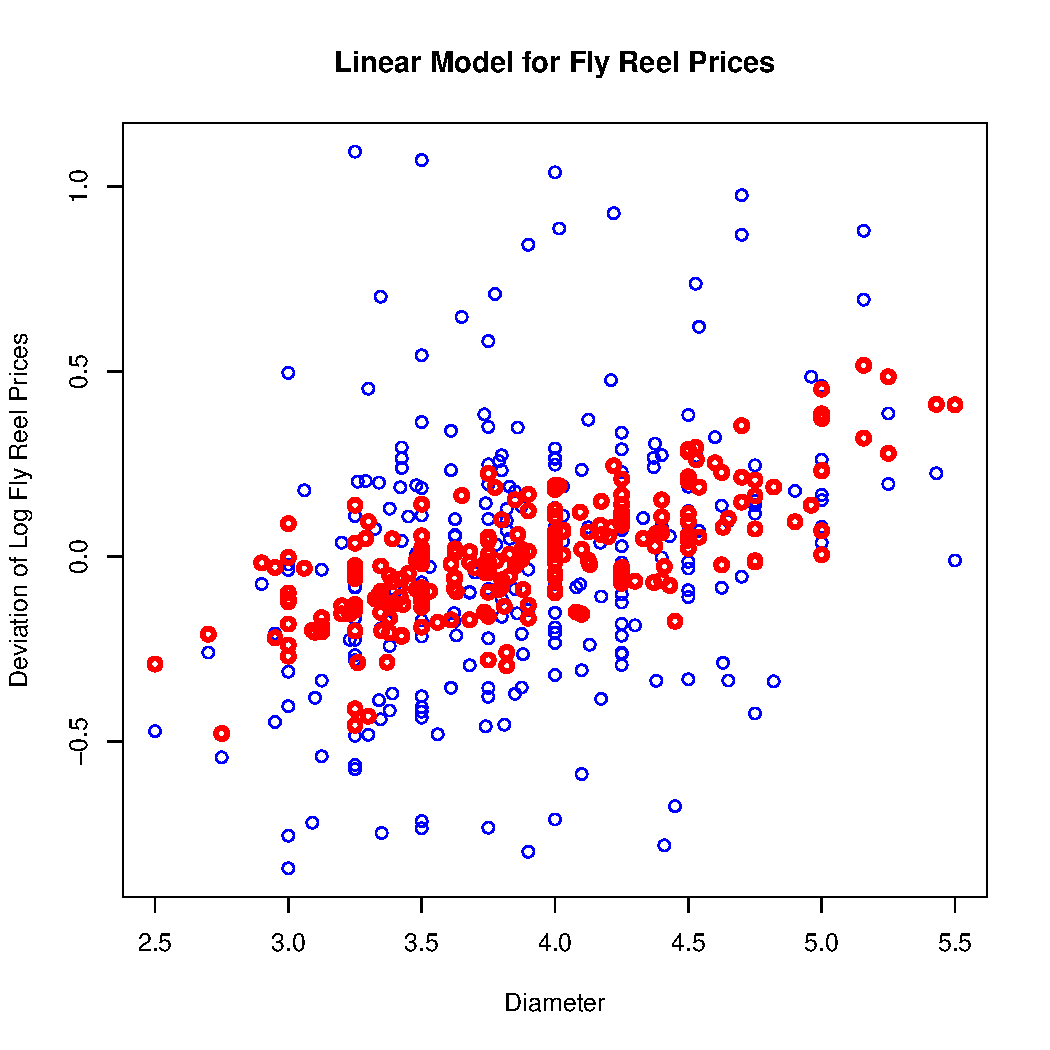
\includegraphics[scale = 0.5, keepaspectratio=true]{../Figures/dev_vs_diameter}
  \caption{Linear Model for Fly Reel Prices vs. Width} \label{fig:dev_vs_width}
\end{figure}



\pagebreak
As a comparison, Figure \ref{fig:dev_np_vs_width_dev} 
augments the above by showing the plot against the 
residuals from the regression for 
width:
the ``excess width'' of a fly reel 
compared to what would be 
expected given the other characteristics of the fly reel. 
The fit follows a straight line, as specified in the model. 
% 
I move directly to the nonparametric specification for 
the relationship between prices and 
width.
Figure \ref{fig:dev_np_vs_width_dev} 
overlays the nonparametric estimate, shown in green. 
The pattern has more variation in slope but 
closely follows the prediction from the linear model. 
Although the nonparametric estimate varies around the linear estimate,
it appears that the linear form
is also a close enough approximation.


\begin{figure}[h!]
  \centering
  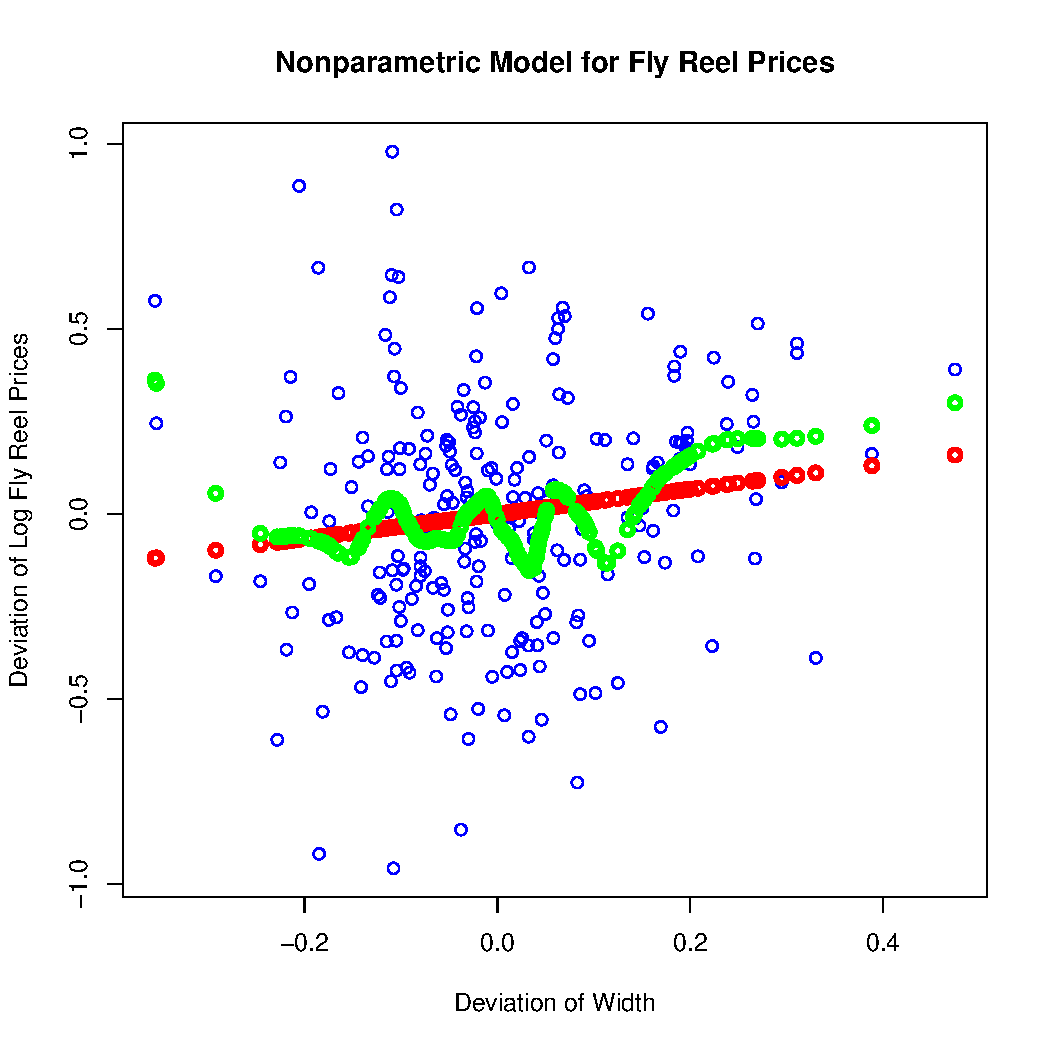
\includegraphics[scale = 0.5, keepaspectratio=true]{../Figures/dev_np_vs_width_dev}
  \caption{Nonparametric Model for Fly Reel Prices: Excess Width} \label{fig:dev_np_vs_width_dev}
\end{figure}


\clearpage
\subsection{Nonparametric Specification for Diameter}

To illustrate the fit of the linear model, 
Figure \ref{fig:dev_vs_diameter} shows a scatter plot 
of the residual log prices on 
the diameter of fly reels. 
The observations are shown in blue
and the fitted values are shown in red.
The variation in the fitted values results from the 
fact that it is not plotted against the transformed 
excess diameter variable 
used in the regressions.
Still, the linear pattern is apparent
and appears to match the data. 

\begin{figure}[h!]
  \centering
  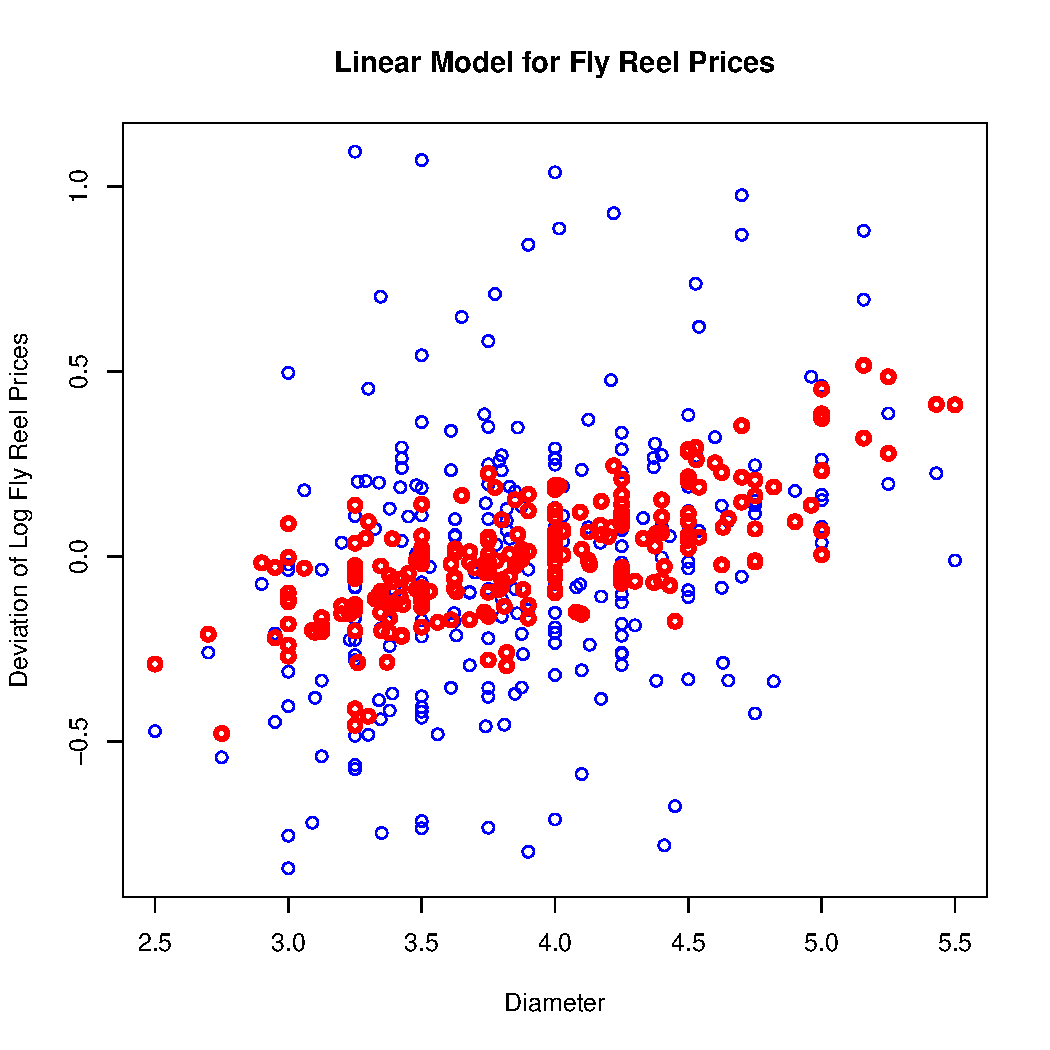
\includegraphics[scale = 0.5, keepaspectratio=true]{../Figures/dev_vs_diameter}
  \caption{Linear Model for Fly Reel Prices vs. Diameter} \label{fig:dev_vs_diameter}
\end{figure}



\pagebreak
As a comparison, Figure \ref{fig:dev_np_vs_diameter_dev} 
augments the above by showing the plot against the 
residuals from the regression for 
diameter:
the ``excess diameter'' of a fly reel 
compared to what would be 
expected given the other characteristics of the fly reel. 
The fit follows a straight line, as specified in the model. 
% 
I move directly to the nonparametric specification for 
the relationship between prices and 
diameter.
Figure \ref{fig:dev_np_vs_diameter_dev} 
overlays the nonparametric estimate, shown in green. 
The pattern has more variation in slope but 
closely follows the prediction from the linear model. 
Although the nonparametric estimate varies around the linear estimate,
it appears that the linear form
is also a close enough approximation.


\begin{figure}[h!]
  \centering
  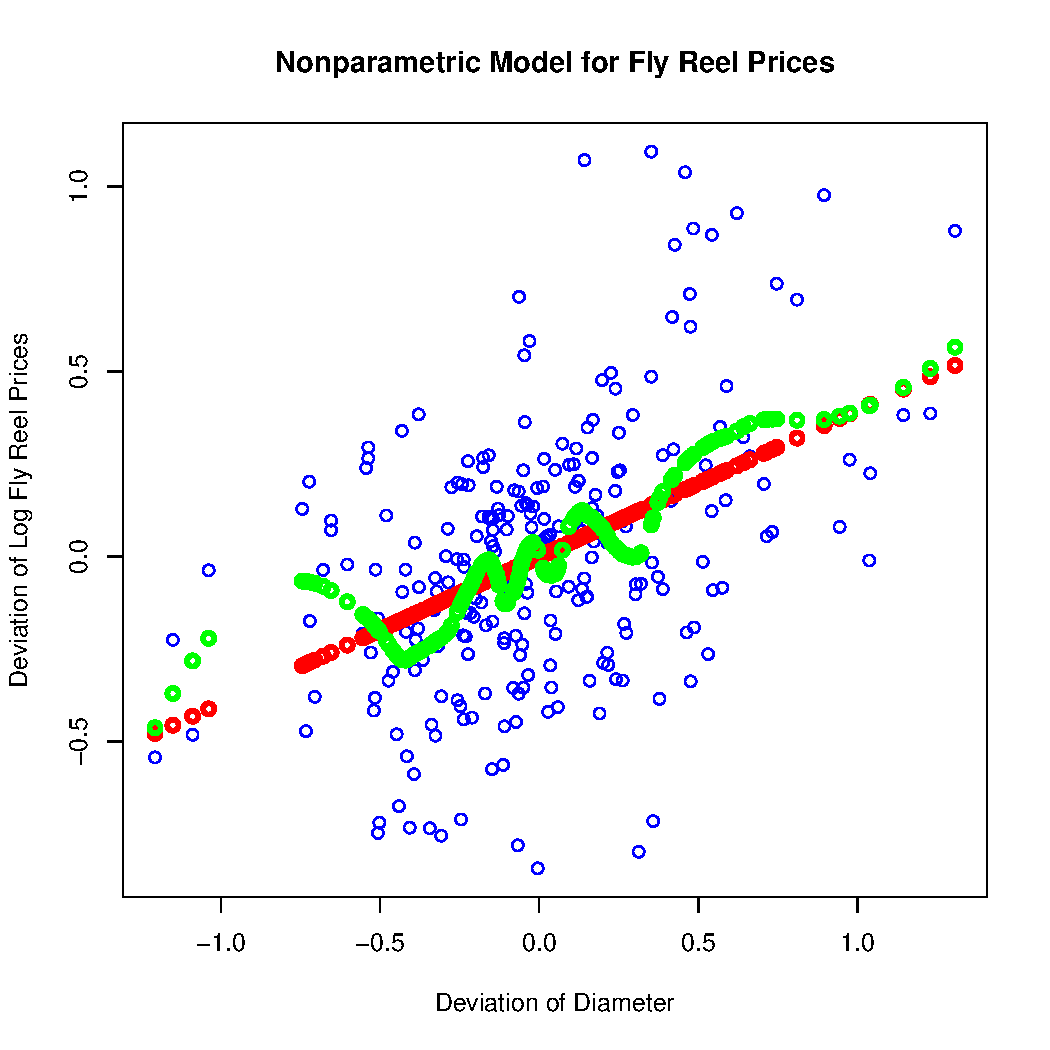
\includegraphics[scale = 0.5, keepaspectratio=true]{../Figures/dev_np_vs_diameter_dev}
  \caption{Nonparametric Model for Fly Reel Prices: Excess Diameter} \label{fig:dev_np_vs_diameter_dev}
\end{figure}



\clearpage
\subsection{Nonparametric Specification for Density}

To illustrate the fit of the linear model, 
Figure \ref{fig:dev_vs_density} shows a scatter plot 
of the residual log prices on 
the density of fly reels. 
The observations are shown in blue
and the fitted values are shown in red.
The variation in the fitted values results from the 
fact that it is not plotted against the transformed 
excess density variable 
used in the regressions.
Still, the linear pattern is apparent
and appears to match the data. 

\begin{figure}[h!]
  \centering
  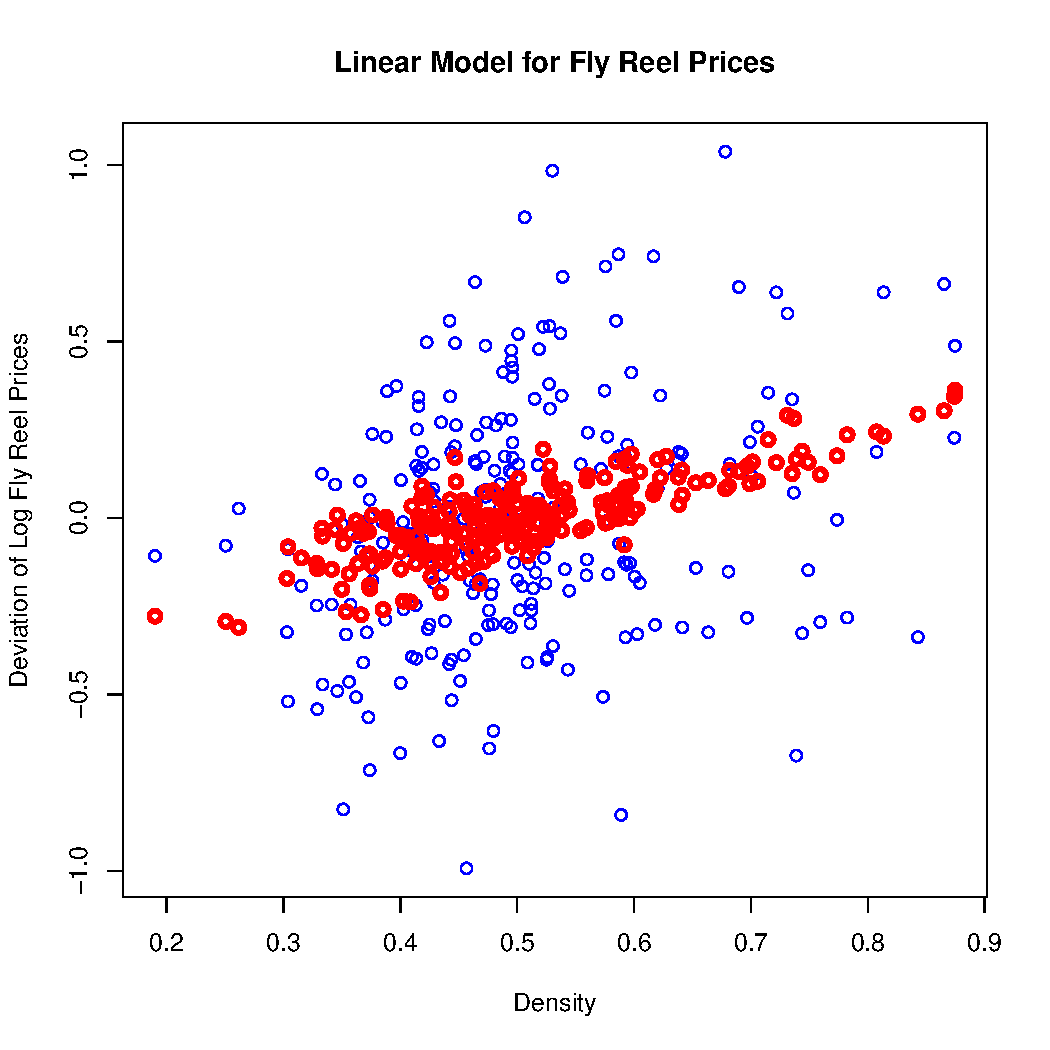
\includegraphics[scale = 0.5, keepaspectratio=true]{../Figures/dev_vs_density}
  \caption{Linear Model for Fly Reel Prices vs. Density} \label{fig:dev_vs_density}
\end{figure}



\pagebreak
As a comparison, Figure \ref{fig:dev_np_vs_density_dev} 
augments the above by showing the plot against the 
residuals from the regression for 
density:
the ``excess density'' of a fly reel 
compared to what would be 
expected given the other characteristics of the fly reel. 
The fit follows a straight line, as specified in the model. 
% 
I move directly to the nonparametric specification for 
the relationship between prices and 
density.
Figure \ref{fig:dev_np_vs_density_dev} 
overlays the nonparametric estimate, shown in green. 
The pattern has more variation in slope but 
closely follows the prediction from the linear model. 
Although the nonparametric estimate varies around the linear estimate,
it appears that the linear form
is also a close enough approximation.


\begin{figure}[h!]
  \centering
  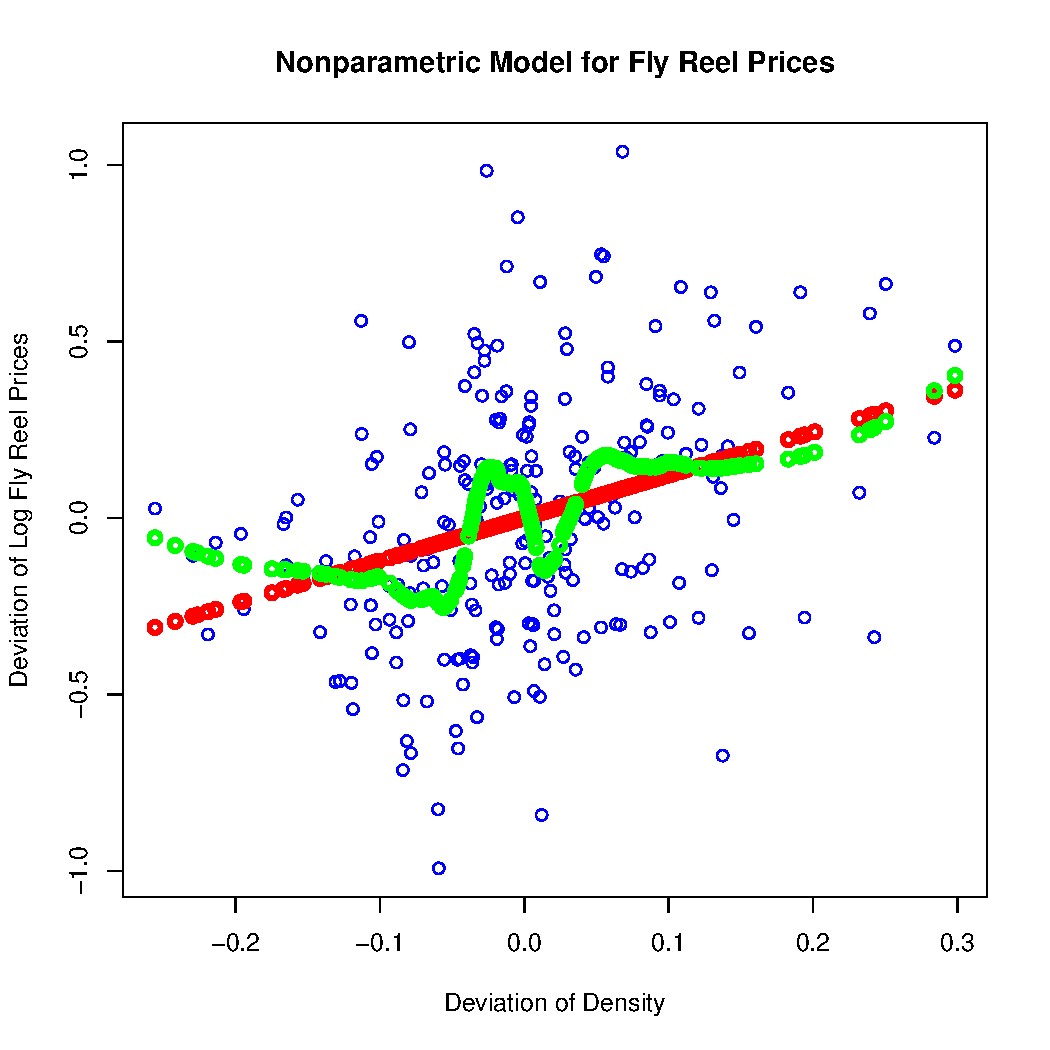
\includegraphics[scale = 0.5, keepaspectratio=true]{../Figures/dev_np_vs_density_dev}
  \caption{Nonparametric Model for Fly Reel Prices: Excess Density} \label{fig:dev_np_vs_density_dev}
\end{figure}

 

\pagebreak
\section{Semiparametric Estimates}

As I was building the above nonparametric models, 
I stored the predictions and will now use them as variables in 
linear models. 
Table \ref{tab:reg_semipar} 
shows the estimates from a set of models. 
Model 1 is the benchmark linear model in 
Table \ref{tab:reg_sealed_USA}. 
Model 2 is a semi-parametric model
with a nonparametric fit on width
substituted in for the width variable.
Models 3 and 4 are semi-parametric models
with nonparametric fits on diameter and density, respectively.
Model 5 is a maximally semiparametric model, 
with nonparametric fits for all continuous variables. 
For each of the single-variable semiparametric models, 
the coefficients are near one
and the fits are similar to the linear model. 
Even with maximal flexibility, the fit of Model 5
is slightly better than the benchmark linear model. 
Across all models, the adjusted $\bar{R}^2$ values are all hovering around 0.75, 
with the full parametric model up to 0.80. 
All things considered, these are excellent models
and the linear model is sufficient
but you might recommend the full semiparametric model
if you can justify the additional complexity.

One factor to keep in mind, however,
is that the above semiparametric models
essentially take the nonparametric functions as known, 
and do not account for the additional variability of
the nonarametric parts of the model.
The next specification estimates both linear 
and nonlinear parts jointly. 


\begin{table}
\begin{center}
\begin{tabular}{l c c c c c}
\hline
 & Model 1 & Model 2 & Model 3 & Model 4 & Model 5 \\
\hline
(Intercept)                 & $2.00999^{***}$ & $2.34926^{***}$ & $2.98091^{***}$  & $3.23438^{***}$ & $4.49531^{***}$  \\
                            & $(0.26125)$     & $(0.22596)$     & $(0.22704)$      & $(0.15261)$     & $(0.05897)$      \\
Width                       & $0.33575^{*}$   &                 & $0.92791^{***}$  & $0.03044$       &                  \\
                            & $(0.15622)$     &                 & $(0.12784)$      & $(0.14082)$     &                  \\
Diameter                    & $0.39567^{***}$ & $0.43144^{***}$ &                  & $0.33658^{***}$ &                  \\
                            & $(0.05076)$     & $(0.04150)$     &                  & $(0.04671)$     &                  \\
Density                     & $1.21296^{***}$ & $1.07566^{***}$ & $0.81613^{***}$  &                 &                  \\
                            & $(0.21948)$     & $(0.20093)$     & $(0.20645)$      &                 &                  \\
SealedYes                   & $0.62731^{***}$ & $0.61960^{***}$ & $0.70050^{***}$  & $0.56858^{***}$ & $0.69858^{***}$  \\
                            & $(0.08622)$     & $(0.08246)$     & $(0.08226)$      & $(0.08047)$     & $(0.07509)$      \\
MachinedYes                 & $0.64934^{***}$ & $0.58954^{***}$ & $0.71659^{***}$  & $0.65070^{***}$ & $0.61103^{***}$  \\
                            & $(0.08320)$     & $(0.07933)$     & $(0.07938)$      & $(0.07819)$     & $(0.07386)$      \\
made\_in\_USATRUE           & $0.74633^{***}$ & $0.77354^{***}$ & $0.79615^{***}$  & $0.70473^{***}$ & $0.79326^{***}$  \\
                            & $(0.09247)$     & $(0.08855)$     & $(0.08879)$      & $(0.08692)$     & $(0.08296)$      \\
SealedYes:made\_in\_USATRUE & $-0.29519^{**}$ & $-0.29826^{**}$ & $-0.33376^{***}$ & $-0.27253^{**}$ & $-0.31356^{***}$ \\
                            & $(0.10092)$     & $(0.09642)$     & $(0.09694)$      & $(0.09500)$     & $(0.09038)$      \\
width\_np                   &                 & $1.11995^{***}$ &                  &                 & $1.35512^{***}$  \\
                            &                 & $(0.21565)$     &                  &                 & $(0.20456)$      \\
diameter\_np                &                 &                 & $1.00650^{***}$  &                 & $1.00083^{***}$  \\
                            &                 &                 & $(0.10926)$      &                 & $(0.10411)$      \\
density\_np                 &                 &                 &                  & $1.03923^{***}$ & $0.76790^{***}$  \\
                            &                 &                 &                  & $(0.12864)$     & $(0.12582)$      \\
\hline
R$^2$                       & $0.74893$       & $0.76995$       & $0.76755$        & $0.77748$       & $0.79771$        \\
Adj. R$^2$                  & $0.74160$       & $0.76324$       & $0.76077$        & $0.77099$       & $0.79181$        \\
Num. obs.                   & $248$           & $248$           & $248$            & $248$           & $248$            \\
\hline
\multicolumn{6}{l}{\scriptsize{$^{***}p<0.001$; $^{**}p<0.01$; $^{*}p<0.05$}}
\end{tabular}
\caption{Semiparametric Models for Fly Reel Prices}
\label{tab:reg_semipar}
\end{center}
\end{table}



\pagebreak
\section{Generalized Additive Model}

\subsection{Linear Model}

As an example of the output from the GAM specification, 
I first estimated the model with no nonlinear terms, 
which is essentially a linear regression. 

\begin{verbatim}
Family: gaussian 
Link function: identity 

Formula:
log_Price ~ Width + Diameter + Density + Sealed + Machined + 
    made_in_USA + made_in_USA * Sealed

Parametric coefficients:
                          Estimate Std. Error t value Pr(>|t|)    
(Intercept)                2.00999    0.26125   7.694 3.69e-13 ***
Width                      0.33575    0.15622   2.149  0.03262 *  
Diameter                   0.39567    0.05076   7.795 1.95e-13 ***
Density                    1.21296    0.21948   5.527 8.49e-08 ***
SealedYes                  0.62731    0.08622   7.275 4.88e-12 ***
MachinedYes                0.64934    0.08320   7.805 1.84e-13 ***
made_in_USATRUE            0.74633    0.09247   8.071 3.35e-14 ***
SealedYes:made_in_USATRUE -0.29519    0.10092  -2.925  0.00378 ** 
---
Signif. codes:  0 �***� 0.001 �**� 0.01 �*� 0.05 �.� 0.1 � � 1


R-sq.(adj) =  0.742   Deviance explained = 74.9%
GCV = 0.10913  Scale est. = 0.10561   n = 248
\end{verbatim}

\pagebreak
\subsection{Semiparametric Model}


Since the results of the full semiparametric specification,
in Model 5 of Table \ref{tab:reg_semipar},
were so promising, 
I estimated the model with all three continuous variables specified as nonparametric functions. 
The result was that 
all the variables---both linear and nonlinear---were 
statistically significant. 
On the other hand, 
the adjusted R-squared has not increased very much, 
from 0.742 to 0.769 under this specification, 
which may not justify the added complexity of the model.
Perhaps more importantly, the coefficients on the 
linear terms are very similar across models, 
indicating that the models support similar conclusions relating to any business decision involving
the ``Made in USA'' premium. 
With this second model, we have even more support for those conclusions
and are certain that the conclusions are not 
coincidental results of the
functional form decisions for previous models.

\begin{verbatim}
Family: gaussian 
Link function: identity 

Formula:
log_saleprice ~ s(horsepower) + s(age) + s(enghours) + diesel + 
    fwd + manual + johndeere + cab

Parametric coefficients:
            Estimate Std. Error t value Pr(>|t|)    
(Intercept)  9.04516    0.09366  96.575  < 2e-16 ***
diesel       0.13440    0.09499   1.415  0.15830    
fwd          0.29899    0.05754   5.196 4.11e-07 ***
manual      -0.16938    0.05965  -2.839  0.00487 ** 
johndeere    0.33067    0.06890   4.799 2.68e-06 ***
cab          0.40439    0.07151   5.655 4.08e-08 ***
---
Signif. codes:  0 �***� 0.001 �**� 0.01 �*� 0.05 �.� 0.1 � � 1

Approximate significance of smooth terms:
                edf Ref.df     F  p-value    
s(horsepower) 4.387  5.321 44.89  < 2e-16 ***
s(age)        3.264  4.057 21.59  < 2e-16 ***
s(enghours)   1.000  1.000 23.39 2.64e-06 ***
---
Signif. codes:  0 �***� 0.001 �**� 0.01 �*� 0.05 �.� 0.1 � � 1

R-sq.(adj) =  0.819   Deviance explained = 82.8%
GCV = 0.15063  Scale est. = 0.14263   n = 276
\end{verbatim}
 

%%%%%%%%%%%%%%%%%%%%%%%%%%%%%%%%%%%%%%%%
\end{document}
%%%%%%%%%%%%%%%%%%%%%%%%%%%%%%%%%%%%%%%%


\pagebreak
\chapter{Transforming the Explanatory Variables}
\documentclass[11pt]{paper}
\usepackage{fullpage}
\usepackage{palatino}
\usepackage{amsfonts,amsmath,amssymb}
% \usepackage{graphicx}

\usepackage{listings}
\usepackage{textcomp}
\usepackage{color}

\definecolor{dkgreen}{rgb}{0,0.6,0}
\definecolor{gray}{rgb}{0.5,0.5,0.5}
\definecolor{mauve}{rgb}{0.58,0,0.82}

\lstset{frame=tb,
  language=R,
  aboveskip=3mm,
  belowskip=3mm,
  showstringspaces=false,
  columns=flexible,
  basicstyle={\small\ttfamily},
  numbers=none,
  numberstyle=\tiny\color{gray},
  keywordstyle=\color{blue},
  commentstyle=\color{dkgreen},
  stringstyle=\color{mauve},
  breaklines=true,
  breakatwhitespace=true,
  tabsize=3
}



\ifx\pdftexversion\undefined
    \usepackage[dvips]{graphicx}
\else
    \usepackage[pdftex]{graphicx}
    \usepackage{epstopdf}
    \epstopdfsetup{suffix=}
\fi

\usepackage{subfig}



% Trying different tips from Google help to get a summary to print.
% \usepackage[T1]{fontenc} 
% \usepackage[utf8]{inputenc}
% 
% \usepackage[utf8]{inputenc}
% \usepackage[utf8x]{inputenc}
\UseRawInputEncoding
% This allows pdflatex to print the curly quotes in the
% significance codes in the output of the GAM.


\begin{document}

%%%%%%%%%%%%%%%%%%%%%%%%%%%%%%%%%%%%%%%%
% Problem Set 7
%%%%%%%%%%%%%%%%%%%%%%%%%%%%%%%%%%%%%%%%

\pagestyle{empty}
{\noindent\bf Spring 2023 \hfill Firstname M.~Lastname}
\vskip 16pt
\centerline{\bf University of Central Florida}
\centerline{\bf College of Business}
\vskip 16pt
\centerline{\bf QMB 6911}
\centerline{\bf Capstone Project in Business Analytics}
\vskip 10pt
\centerline{\bf Solutions:  Problem Set \#7}
\vskip 32pt
\noindent
% 
% 
\section{Data Description}
% 
By engaging an industry consultant to gather relevant and appropriate 
information, your firm has been able to put together data concerning 248 
different fly-fishing reels, over one-half of which are produced in the 
United States, with the remainder being produced in Asia---either in China 
or Korea.  These data are contained in the file {\tt FlyReels.csv}, which is
available in the {\tt Data} folder.
Each fly-fishing reel in the data set is a row, while the columns correspond 
to the variables whose names and definitions are the following:
\bigskip
\begin{table}[ht]
\centering
\begin{tabular}{ll}
  \hline
    Variable & Definition \\
  \hline

    {\tt Name}        &product name (a string) \\ 
    {\tt Brand}       &brand name (a string) \\ 
    {\tt Weight}      &weight of reel in ounces (a real number) \\ 
    {\tt Diameter}    &diameter of reel in inches (a real number) \\ 
    {\tt Width}       &width of reel in inches (a real number) \\ 
    {\tt Price}       &price of reel in dollars (a real number) \\ 
    {\tt Sealed}      &whether the reel is sealed; {\tt "Yes"} versus
                        {\tt "No"} (a string) \\ 
    {\tt Country}     &country of manufacture, (a string) \\ 
    {\tt Machined}    &whether the reel is machined versus cast;
                        machined={\tt "Yes"}, \\ 
                      &while cast={\tt "No"} (a string) \\ 
  \hline
\end{tabular}
%\caption{Summary of Numeric Variables}
%\label{tab:summary}
\end{table}


I will revisit the recommended linear model
from Problem Set \#7
and the semiparametric specifications, 
which we covered for Problem Set \#8. 



Then I will further investigate any nonlinear relationships
by incorporating a nonlinear but parametric specification
for the value of the dimensions of the reels:
the width, diameter, and density, 
which constitute the continuous variables in the dataset.
This parametric analysis will be performed
using the Box-Tidwell framework
to investigate whether the value of these characteristics
are best described with parametric nonlinear forms. 


%%%%%%%%%%%%%%%%%%%%%%%%%%%%%%%%%%%%%%%%
\clearpage
\section{Linear Regression Model}
%%%%%%%%%%%%%%%%%%%%%%%%%%%%%%%%%%%%%%%%

A natural staring point is the recommended linear model
from Problem Set \#7. 

\subsection{Linear Model with \texttt{Sealed*Made\_in\_USA} Interaction}

Last week I investigated whether 
the functional form should include different specifications by
country of manufacture.
% 
The model included the continuous variables 
width, diameter, and density, 
as well as categorical variables for 
country of manufacture, 
and whether or not the reels were sealed or machined. 
% 
In addition to the indicator for the country of manufacture, the model included an indicator for an interaction between
the the country of manufacture indicator and the indicator for whether the reels were sealed or unsealed. 
% 
The dependent variable was chosen as 
the logarithm of the fly reel price, 
since the results were similar to those from the model 
with the optimal Box-Cox transformation, 
without the added complexity. 
% 
The results of this regression specification are shown in 
Table \ref{tab:reg_sealed_USA}. 
% 

\begin{table}
\begin{center}
\begin{tabular}{l c}
\hline
 & Model 1 \\
\hline
(Intercept)                 & $2.00999^{***}$ \\
                            & $(0.26125)$     \\
Width                       & $0.33575^{*}$   \\
                            & $(0.15622)$     \\
Diameter                    & $0.39567^{***}$ \\
                            & $(0.05076)$     \\
Density                     & $1.21296^{***}$ \\
                            & $(0.21948)$     \\
SealedYes                   & $0.62731^{***}$ \\
                            & $(0.08622)$     \\
MachinedYes                 & $0.64934^{***}$ \\
                            & $(0.08320)$     \\
made\_in\_USATRUE           & $0.74633^{***}$ \\
                            & $(0.09247)$     \\
SealedYes:made\_in\_USATRUE & $-0.29519^{**}$ \\
                            & $(0.10092)$     \\
\hline
R$^2$                       & $0.74893$       \\
Adj. R$^2$                  & $0.74160$       \\
Num. obs.                   & $248$           \\
\hline
\multicolumn{2}{l}{\scriptsize{$^{***}p<0.001$; $^{**}p<0.01$; $^{*}p<0.05$}}
\end{tabular}
\caption{Linear Model for Fly Reel Prices}
\label{tab:reg_sealed_USA}
\end{center}
\end{table}

% 
Next, I will attempt to improve on this specification
by investigating the potential for nonlinear functional forms, 
as we did for Problem Set \#8. 







%%%%%%%%%%%%%%%%%%%%%%%%%%%%%%%%%%%%%%%%
\clearpage
\section{Nonlinear Specifications}
%%%%%%%%%%%%%%%%%%%%%%%%%%%%%%%%%%%%%%%%


% \clearpage
\subsection{Nonparametric Specification for Width}

As above, I first conducted FWL regressions 
to reduce the problem to two dimensions. 
The results are not shown here, 
since the comparison only verifies 
the conclusion of the FWL theorem. 

To illustrate the fit of the linear model, 
Figure \ref{fig:dev_np_vs_width_dev} 
shows a scatter plot 
of the residual log prices on 
residuals from the regression for 
width:
the ``excess width'' of a fly reel 
compared to what would be 
expected given the other characteristics of the fly reel. 
The observations are shown in blue
and the fitted values from the linear model are shown in red.
The fit follows a straight line, as expected for a linear model. 

% 
I move directly to the nonparametric specification for 
the relationship between prices and 
width.
Figure \ref{fig:dev_np_vs_width_dev} 
overlays the nonparametric estimate, shown in green. 
The pattern has more variation in slope but 
closely follows the prediction from the linear model. 
Although the nonparametric estimate varies around the linear estimate,
it appears that the linear form
is also a close enough approximation.


\begin{figure}[h!]
  \centering
  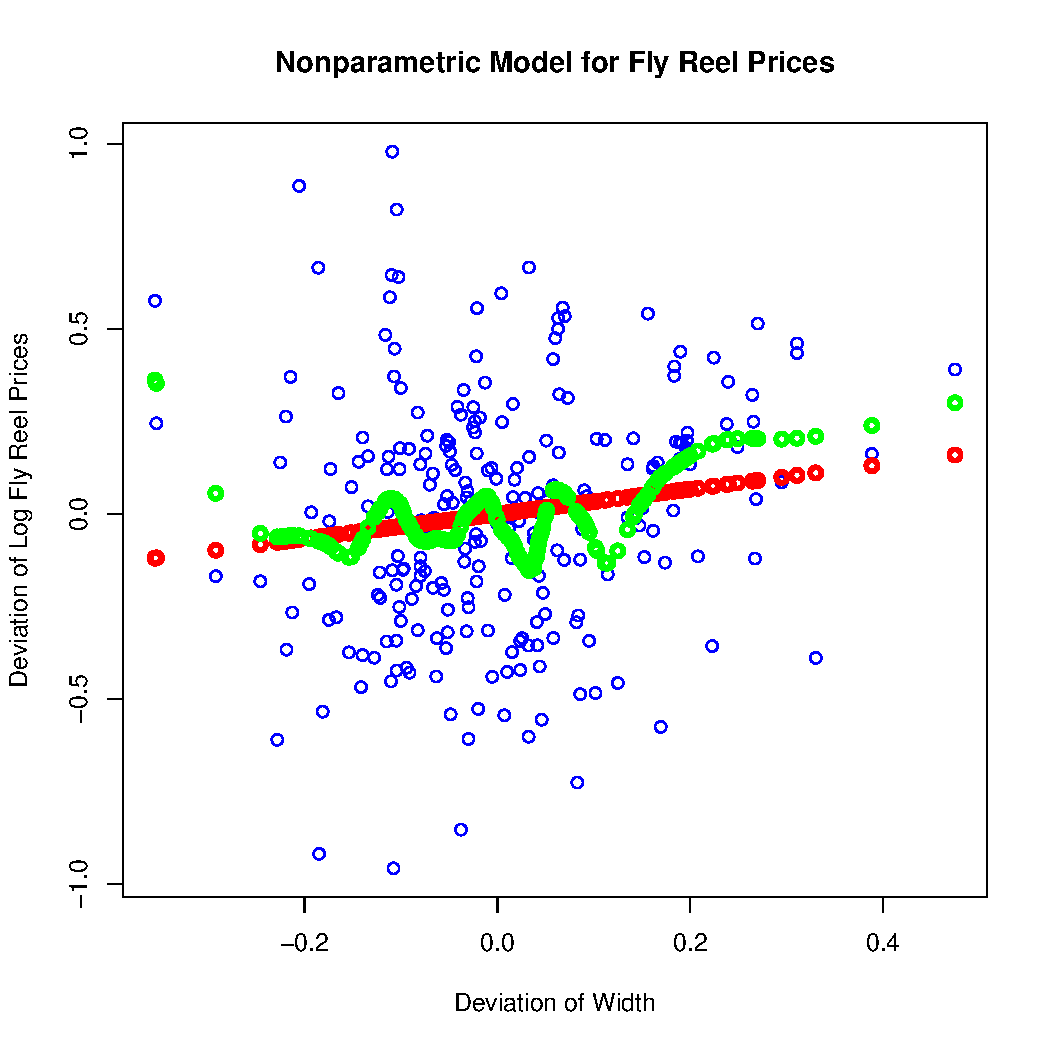
\includegraphics[scale = 0.5, keepaspectratio=true]{../Figures/dev_np_vs_width_dev}
  \caption{Nonparametric Model for Fly Reel Prices: Excess Width} \label{fig:dev_np_vs_width_dev}
\end{figure}


\clearpage
\subsection{Nonparametric Specification for Diameter}

To illustrate the fit of the linear model, 
Figure \ref{fig:dev_np_vs_diameter_dev} 
shows a scatter plot 
of the residual log prices on 
residuals from the regression for 
diameter:
the ``excess diameter'' of a fly reel 
compared to what would be 
expected given the other characteristics of the fly reel. 
The observations are shown in blue
and the fitted values from the linear model are shown in red.
The fit follows a straight line, as expected for a linear model. 

% 
I move directly to the nonparametric specification for 
the relationship between prices and 
diameter.
Figure \ref{fig:dev_np_vs_diameter_dev} 
overlays the nonparametric estimate, shown in green. 
The pattern has more variation in slope but 
closely follows the prediction from the linear model. 
Although the nonparametric estimate varies around the linear estimate,
it appears that the linear form
is also a close enough approximation.


\begin{figure}[h!]
  \centering
  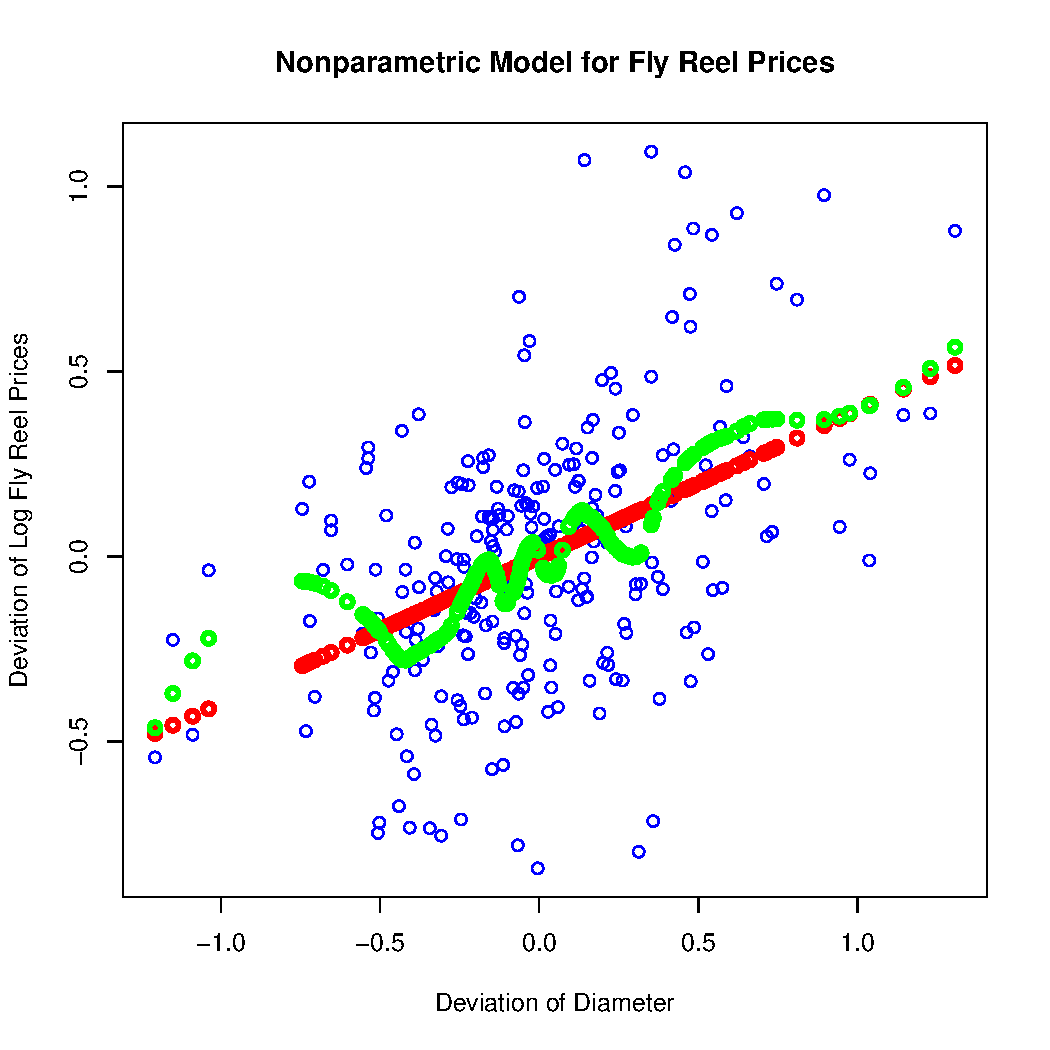
\includegraphics[scale = 0.5, keepaspectratio=true]{../Figures/dev_np_vs_diameter_dev}
  \caption{Nonparametric Model for Fly Reel Prices: Excess Diameter} \label{fig:dev_np_vs_diameter_dev}
\end{figure}



\clearpage
\subsection{Nonparametric Specification for Density}

To illustrate the fit of the linear model, 
Figure \ref{fig:dev_np_vs_density_dev} 
shows a scatter plot 
of the residual log prices on 
residuals from the regression for 
density:
the ``excess density'' of a fly reel 
compared to what would be 
expected given the other characteristics of the fly reel. 
The observations are shown in blue
and the fitted values are shown in red.
The fit follows a straight line, as expected for a linear model. 

% 
I move directly to the nonparametric specification for 
the relationship between prices and 
density.
Figure \ref{fig:dev_np_vs_density_dev} 
overlays the nonparametric estimate, shown in green. 
The pattern has more variation in slope but 
closely follows the prediction from the linear model. 
Although the nonparametric estimate varies around the linear estimate,
it appears that the linear form
is also a close enough approximation.


\begin{figure}[h!]
  \centering
  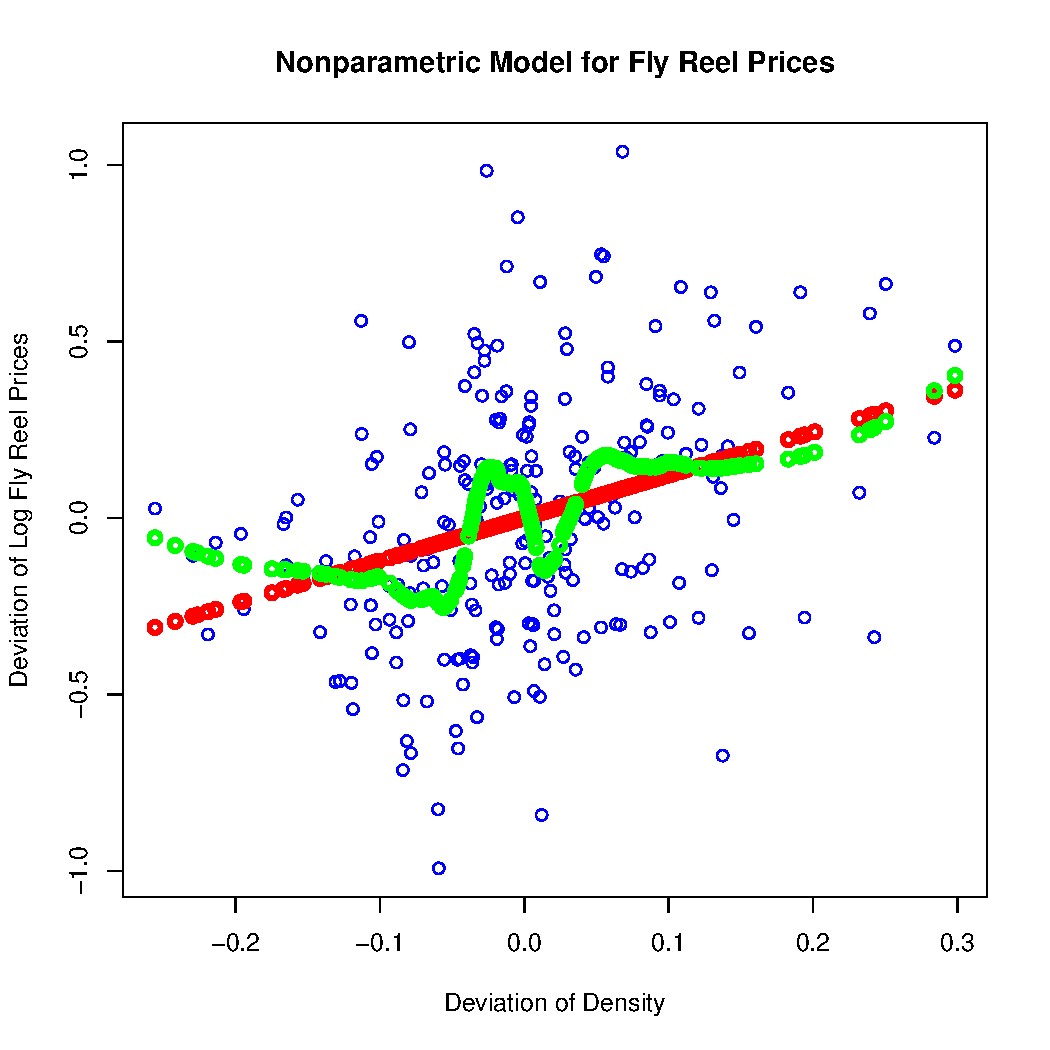
\includegraphics[scale = 0.5, keepaspectratio=true]{../Figures/dev_np_vs_density_dev}
  \caption{Nonparametric Model for Fly Reel Prices: Excess Density} \label{fig:dev_np_vs_density_dev}
\end{figure}

 

\pagebreak
\section{Semiparametric Estimates}

As I was building the above nonparametric models, 
I stored the predictions and will used them as variables in 
linear models. 
Table \ref{tab:reg_semipar} 
shows the estimates from a set of models. 
Model 1 is the benchmark linear model in 
Table \ref{tab:reg_sealed_USA}. 
Model 2 is a semi-parametric model
with a nonparametric fit on width
substituted in for the width variable.
Models 3 and 4 are semi-parametric models
with nonparametric fits on diameter and density, respectively.
Model 5 is a maximally semiparametric model, 
with nonparametric fits for all continuous variables. 
For each of the single-variable semiparametric models, 
the coefficients are near one
and the fits are similar to the linear model. 
Even with maximal flexibility, the fit of Model 5
is slightly better than the benchmark linear model. 
Across all models, the adjusted $\bar{R}^2$ values are all hovering around 0.75, 
with the full parametric model up to 0.80. 
All things considered, these are excellent models
and the linear model is sufficient
but you might recommend the full semiparametric model
if you can justify the additional complexity.

One factor to keep in mind, however,
is that the above semiparametric models
essentially take the nonparametric functions as known, 
and do not account for the additional variability of
the nonarametric parts of the model.
The next specification estimates both linear 
and nonlinear parts jointly. 


\begin{table}
\begin{center}
\begin{tabular}{l c c c c c}
\hline
 & Model 1 & Model 2 & Model 3 & Model 4 & Model 5 \\
\hline
(Intercept)                 & $2.00999^{***}$ & $2.34926^{***}$ & $2.98091^{***}$  & $3.23438^{***}$ & $4.49531^{***}$  \\
                            & $(0.26125)$     & $(0.22596)$     & $(0.22704)$      & $(0.15261)$     & $(0.05897)$      \\
Width                       & $0.33575^{*}$   &                 & $0.92791^{***}$  & $0.03044$       &                  \\
                            & $(0.15622)$     &                 & $(0.12784)$      & $(0.14082)$     &                  \\
Diameter                    & $0.39567^{***}$ & $0.43144^{***}$ &                  & $0.33658^{***}$ &                  \\
                            & $(0.05076)$     & $(0.04150)$     &                  & $(0.04671)$     &                  \\
Density                     & $1.21296^{***}$ & $1.07566^{***}$ & $0.81613^{***}$  &                 &                  \\
                            & $(0.21948)$     & $(0.20093)$     & $(0.20645)$      &                 &                  \\
SealedYes                   & $0.62731^{***}$ & $0.61960^{***}$ & $0.70050^{***}$  & $0.56858^{***}$ & $0.69858^{***}$  \\
                            & $(0.08622)$     & $(0.08246)$     & $(0.08226)$      & $(0.08047)$     & $(0.07509)$      \\
MachinedYes                 & $0.64934^{***}$ & $0.58954^{***}$ & $0.71659^{***}$  & $0.65070^{***}$ & $0.61103^{***}$  \\
                            & $(0.08320)$     & $(0.07933)$     & $(0.07938)$      & $(0.07819)$     & $(0.07386)$      \\
made\_in\_USATRUE           & $0.74633^{***}$ & $0.77354^{***}$ & $0.79615^{***}$  & $0.70473^{***}$ & $0.79326^{***}$  \\
                            & $(0.09247)$     & $(0.08855)$     & $(0.08879)$      & $(0.08692)$     & $(0.08296)$      \\
SealedYes:made\_in\_USATRUE & $-0.29519^{**}$ & $-0.29826^{**}$ & $-0.33376^{***}$ & $-0.27253^{**}$ & $-0.31356^{***}$ \\
                            & $(0.10092)$     & $(0.09642)$     & $(0.09694)$      & $(0.09500)$     & $(0.09038)$      \\
width\_np                   &                 & $1.11995^{***}$ &                  &                 & $1.35512^{***}$  \\
                            &                 & $(0.21565)$     &                  &                 & $(0.20456)$      \\
diameter\_np                &                 &                 & $1.00650^{***}$  &                 & $1.00083^{***}$  \\
                            &                 &                 & $(0.10926)$      &                 & $(0.10411)$      \\
density\_np                 &                 &                 &                  & $1.03923^{***}$ & $0.76790^{***}$  \\
                            &                 &                 &                  & $(0.12864)$     & $(0.12582)$      \\
\hline
R$^2$                       & $0.74893$       & $0.76995$       & $0.76755$        & $0.77748$       & $0.79771$        \\
Adj. R$^2$                  & $0.74160$       & $0.76324$       & $0.76077$        & $0.77099$       & $0.79181$        \\
Num. obs.                   & $248$           & $248$           & $248$            & $248$           & $248$            \\
\hline
\multicolumn{6}{l}{\scriptsize{$^{***}p<0.001$; $^{**}p<0.01$; $^{*}p<0.05$}}
\end{tabular}
\caption{Semiparametric Models for Fly Reel Prices}
\label{tab:reg_semipar}
\end{center}
\end{table}



\pagebreak
\section{Generalized Additive Model}

\subsection{Linear Model}

As an example of the output from the GAM specification, 
I first estimated the model with no nonlinear terms, 
which is essentially a linear regression. 

\begin{verbatim}
Family: gaussian 
Link function: identity 

Formula:
log_Price ~ Width + Diameter + Density + Sealed + Machined + 
    made_in_USA + made_in_USA * Sealed

Parametric coefficients:
                          Estimate Std. Error t value Pr(>|t|)    
(Intercept)                2.00999    0.26125   7.694 3.69e-13 ***
Width                      0.33575    0.15622   2.149  0.03262 *  
Diameter                   0.39567    0.05076   7.795 1.95e-13 ***
Density                    1.21296    0.21948   5.527 8.49e-08 ***
SealedYes                  0.62731    0.08622   7.275 4.88e-12 ***
MachinedYes                0.64934    0.08320   7.805 1.84e-13 ***
made_in_USATRUE            0.74633    0.09247   8.071 3.35e-14 ***
SealedYes:made_in_USATRUE -0.29519    0.10092  -2.925  0.00378 ** 
---
Signif. codes:  0 �***� 0.001 �**� 0.01 �*� 0.05 �.� 0.1 � � 1


R-sq.(adj) =  0.742   Deviance explained = 74.9%
GCV = 0.10913  Scale est. = 0.10561   n = 248
\end{verbatim}

\pagebreak
\subsection{Semiparametric Model}


Since the results of the full semiparametric specification,
in Model 5 of Table \ref{tab:reg_semipar},
were so promising, 
I estimated the model with all three continuous variables specified as nonparametric functions. 
The result was that 
all the variables---both linear and nonlinear---were 
statistically significant. 
On the other hand, 
the adjusted R-squared has not increased very much, 
from 0.742 to 0.769 under this specification, 
which may not justify the added complexity of the model.
Perhaps more importantly, the coefficients on the 
linear terms are very similar across models, 
indicating that the models support similar conclusions relating to any business decision involving
the ``Made in USA'' premium. 
With this second model, we have even more support for those conclusions
and are certain that the conclusions are not 
coincidental results of the
functional form decisions for previous models.

\begin{verbatim}
Family: gaussian 
Link function: identity 

Formula:
log_saleprice ~ s(horsepower) + s(age) + s(enghours) + diesel + 
    fwd + manual + johndeere + cab

Parametric coefficients:
            Estimate Std. Error t value Pr(>|t|)    
(Intercept)  9.04516    0.09366  96.575  < 2e-16 ***
diesel       0.13440    0.09499   1.415  0.15830    
fwd          0.29899    0.05754   5.196 4.11e-07 ***
manual      -0.16938    0.05965  -2.839  0.00487 ** 
johndeere    0.33067    0.06890   4.799 2.68e-06 ***
cab          0.40439    0.07151   5.655 4.08e-08 ***
---
Signif. codes:  0 �***� 0.001 �**� 0.01 �*� 0.05 �.� 0.1 � � 1

Approximate significance of smooth terms:
                edf Ref.df     F  p-value    
s(horsepower) 4.387  5.321 44.89  < 2e-16 ***
s(age)        3.264  4.057 21.59  < 2e-16 ***
s(enghours)   1.000  1.000 23.39 2.64e-06 ***
---
Signif. codes:  0 �***� 0.001 �**� 0.01 �*� 0.05 �.� 0.1 � � 1

R-sq.(adj) =  0.819   Deviance explained = 82.8%
GCV = 0.15063  Scale est. = 0.14263   n = 276
\end{verbatim}
 



\pagebreak
\section{The Box--Tidwell Transformation}

The Box--Tidwell function tests for non-linear relationships
to the mean of the dependent variable.
The nonlinearity is in the form of an
exponential transformation in the form of the Box-Cox
transformation, except that the transformation is taken
on the explanatory variables.


\subsection{Transformation of Width}


Performing the transformation on the 
width variable
produces a modified form of the linear model.
This specification allows a single exponential
transformation on 
width, 
rather than a linear form.

\begin{verbatim} MLE of lambda Score Statistic (z) Pr(>|z|)
        1.1615              0.1587   0.8739

iterations =  5 
\end{verbatim}

The \textsf{R} output is the statistics for a test of nonlinearity:
that the exponent $\lambda$ in the Box--Tidwell transformation is zero.
%
The "\texttt{MLE of lambda}" statistic is the optimal exponent on horsepower.
Similar to the Box-Cox transformation,
with Box-Tidwell, the exponents are on the explanatory variables
and are all called lambda, in contrast
to the parameter $\tau$ in our class notes.
%  
The exponent is not significantly different from one. 
This supports a linear form for Width,
confirming our result from the nonparametric analysis.



\subsection{Transformation of Diameter}


\begin{verbatim} MLE of lambda Score Statistic (z) Pr(>|z|)
      -0.35213             -1.2106    0.226

iterations =  4 
\end{verbatim}


This is very weak evidence for
an inverse square root transformation
for diameter but it is not estimated accurately.
%
There is no evidence for a transformation 
with a coefficient different from 1, 
which suggests
a purely linear relationship between \texttt{log\_Price}
and 
diameter.
Next, I will consider the possibility of nonlinearity 
in the value of the density of a reel. 

\subsection{Transformation of Density}


\begin{verbatim} MLE of lambda Score Statistic (z) Pr(>|z|)
       0.19315             -1.3448   0.1787

iterations =  10 
\end{verbatim}

Similar to Diameter, this is very weak evidence for
a square root transformation
for diameter but it is not estimated accurately.
%
Conclude that the linear model is the best choice.






%%%%%%%%%%%%%%%%%%%%%%%%%%%%%%%%%%%%%%%%
\end{document}
%%%%%%%%%%%%%%%%%%%%%%%%%%%%%%%%%%%%%%%%


\pagebreak
\chapter{Sample Selection Models}
\documentclass[11pt]{paper}
\usepackage{fullpage}
\usepackage{palatino}
\usepackage{amsfonts,amsmath,amssymb}
% \usepackage{graphicx}

\usepackage{listings}
\usepackage{textcomp}
\usepackage{color}

\definecolor{dkgreen}{rgb}{0,0.6,0}
\definecolor{gray}{rgb}{0.5,0.5,0.5}
\definecolor{mauve}{rgb}{0.58,0,0.82}

\lstset{frame=tb,
  language=R,
  aboveskip=3mm,
  belowskip=3mm,
  showstringspaces=false,
  columns=flexible,
  basicstyle={\small\ttfamily},
  numbers=none,
  numberstyle=\tiny\color{gray},
  keywordstyle=\color{blue},
  commentstyle=\color{dkgreen},
  stringstyle=\color{mauve},
  breaklines=true,
  breakatwhitespace=true,
  tabsize=3
}



\ifx\pdftexversion\undefined
    \usepackage[dvips]{graphicx}
\else
    \usepackage[pdftex]{graphicx}
    \usepackage{epstopdf}
    \epstopdfsetup{suffix=}
\fi

\usepackage{subfig}



% Trying different tips from Google help to get a summary to print.
% \usepackage[T1]{fontenc} 
% \usepackage[utf8]{inputenc}
% 
% \usepackage[utf8]{inputenc}
% \usepackage[utf8x]{inputenc}
\UseRawInputEncoding
% This allows pdflatex to print the curly quotes in the
% significance codes in the output of the GAM.


\begin{document}

%%%%%%%%%%%%%%%%%%%%%%%%%%%%%%%%%%%%%%%%
% Problem Set 7
%%%%%%%%%%%%%%%%%%%%%%%%%%%%%%%%%%%%%%%%

\pagestyle{empty}
{\noindent\bf Spring 2021 \hfill Firstname M.~Lastname}
\vskip 16pt
\centerline{\bf University of Central Florida}
\centerline{\bf College of Business}
\vskip 16pt
\centerline{\bf QMB 6911}
\centerline{\bf Capstone Project in Business Analytics}
\vskip 10pt
\centerline{\bf Solutions:  Problem Set \#10}
\vskip 32pt
\noindent
% 
% 
\section{Data Description}
% 
By engaging an industry consultant to gather relevant and appropriate 
information, your firm has been able to put together data concerning 248 
different fly-fishing reels, over one-half of which are produced in the 
United States, with the remainder being produced in Asia---either in China 
or Korea.  These data are contained in the file {\tt FlyReels.csv}, which is
available in the {\tt Data} folder.
Each fly-fishing reel in the data set is a row, while the columns correspond 
to the variables whose names and definitions are the following:
\bigskip
\begin{table}[ht]
\centering
\begin{tabular}{ll}
  \hline
    Variable & Definition \\
  \hline

    {\tt Name}        &product name (a string) \\ 
    {\tt Brand}       &brand name (a string) \\ 
    {\tt Weight}      &weight of reel in ounces (a real number) \\ 
    {\tt Diameter}    &diameter of reel in inches (a real number) \\ 
    {\tt Width}       &width of reel in inches (a real number) \\ 
    {\tt Price}       &price of reel in dollars (a real number) \\ 
    {\tt Sealed}      &whether the reel is sealed; {\tt "Yes"} versus
                        {\tt "No"} (a string) \\ 
    {\tt Country}     &country of manufacture, (a string) \\ 
    {\tt Machined}    &whether the reel is machined versus cast;
                        machined={\tt "Yes"}, \\ 
                      &while cast={\tt "No"} (a string) \\ 
  \hline
\end{tabular}
%\caption{Summary of Numeric Variables}
%\label{tab:summary}
\end{table}


I will revisit the recommended linear model
from Problem Set \#7, 
which was supported in
Problem Sets \#8 and  \#9 
by considering other nonlinear specifications
within a Generalized Additive Model. 



Then I will further investigate this nonlinear relationship
by considering the issue of sample selection:
fly reel manufacturers 
may produce 
fly reels in each country
with specific qualities based on
their perceived value to typical 
American 
customers, 
in ways that are not represented by the variables in the dataset.



%%%%%%%%%%%%%%%%%%%%%%%%%%%%%%%%%%%%%%%%
\clearpage
\section{Linear Regression Model}
%%%%%%%%%%%%%%%%%%%%%%%%%%%%%%%%%%%%%%%%

A natural staring point is the recommended linear model
from Problem Set \#7. 

\subsection{Linear Model with \texttt{Sealed*Made\_in\_USA} Interaction}

Last week I investigated whether 
the functional form should include different specifications by
country of manufacture.
% 
The model included the continuous variables 
width, diameter, and density, 
as well as categorical variables for 
country of manufacture, 
and whether or not the reels were sealed or machined. 
% 
In addition to the indicator for the country of manufacture, the model included an indicator for an interaction between
the the country of manufacture indicator and the indicator for whether the reels were sealed or unsealed. 
% 
The dependent variable was chosen as 
the logarithm of the fly reel price, 
since the results were similar to those from the model 
with the optimal Box-Cox transformation, 
without the added complexity. 
% 
The results of this regression specification are shown in 
Table \ref{tab:reg_sealed_USA}. 
% 

\begin{table}
\begin{center}
\begin{tabular}{l c}
\hline
 & Model 1 \\
\hline
(Intercept)                 & $2.00999^{***}$ \\
                            & $(0.26125)$     \\
Width                       & $0.33575^{*}$   \\
                            & $(0.15622)$     \\
Diameter                    & $0.39567^{***}$ \\
                            & $(0.05076)$     \\
Density                     & $1.21296^{***}$ \\
                            & $(0.21948)$     \\
SealedYes                   & $0.62731^{***}$ \\
                            & $(0.08622)$     \\
MachinedYes                 & $0.64934^{***}$ \\
                            & $(0.08320)$     \\
made\_in\_USATRUE           & $0.74633^{***}$ \\
                            & $(0.09247)$     \\
SealedYes:made\_in\_USATRUE & $-0.29519^{**}$ \\
                            & $(0.10092)$     \\
\hline
R$^2$                       & $0.74893$       \\
Adj. R$^2$                  & $0.74160$       \\
Num. obs.                   & $248$           \\
\hline
\multicolumn{2}{l}{\scriptsize{$^{***}p<0.001$; $^{**}p<0.01$; $^{*}p<0.05$}}
\end{tabular}
\caption{Linear Model for Fly Reel Prices}
\label{tab:reg_sealed_USA}
\end{center}
\end{table}

% 
Next, I will attempt to improve on this specification,
using Tobit models for sample selection.





%%%%%%%%%%%%%%%%%%%%%%%%%%%%%%%%%%%%%%%%
\pagebreak
\subsection{Comparison by Country of Manufacture}
%%%%%%%%%%%%%%%%%%%%%%%%%%%%%%%%%%%%%%%%

Table \ref{tab:reg_by_country} shows the results of 
a series of regression models 
on different samples by country of manufacture.
Model 1 shows the results 
for the full model
using the sample of fly reels made in the USA
and Model 3 shows the remaining fly reels made in China or Korea.
Models 2 and 4 show the estimates from a reduced model
on each sample, eliminating the variable \texttt{Width}, 
which was not significant in either of these smaller samples.


\begin{table}
\begin{center}
\begin{tabular}{l c c c c}
\hline
 & Model 1 & Model 2 & Model 3 & Model 4 \\
\hline
(Intercept) & $3.35^{***}$ & $3.48^{***}$ & $2.03^{***}$ & $2.41^{***}$ \\
            & $(0.30)$     & $(0.28)$     & $(0.47)$     & $(0.41)$     \\
Width       & $0.28$       &              & $0.39$       &              \\
            & $(0.22)$     &              & $(0.23)$     &              \\
Diameter    & $0.44^{***}$ & $0.49^{***}$ & $0.36^{***}$ & $0.41^{***}$ \\
            & $(0.07)$     & $(0.05)$     & $(0.08)$     & $(0.07)$     \\
Density     & $1.13^{***}$ & $1.06^{***}$ & $1.32^{**}$  & $1.06^{**}$  \\
            & $(0.25)$     & $(0.25)$     & $(0.41)$     & $(0.38)$     \\
SealedYes   & $0.32^{***}$ & $0.32^{***}$ & $0.65^{***}$ & $0.64^{***}$ \\
            & $(0.06)$     & $(0.06)$     & $(0.10)$     & $(0.10)$     \\
MachinedYes &              &              & $0.65^{***}$ & $0.63^{***}$ \\
            &              &              & $(0.09)$     & $(0.09)$     \\
\hline
R$^2$       & $0.54$       & $0.53$       & $0.75$       & $0.74$       \\
Adj. R$^2$  & $0.52$       & $0.52$       & $0.73$       & $0.73$       \\
Num. obs.   & $135$        & $135$        & $113$        & $113$        \\
\hline
\multicolumn{5}{l}{\scriptsize{$^{***}p<0.001$; $^{**}p<0.01$; $^{*}p<0.05$}}
\end{tabular}
\caption{Regression Models by Country of Manufacture}
\label{tab:reg_by_country}
\end{center}
\end{table}


The width of the reel is insignificant in both samples
and the coefficients are qualitatively similar across the samples, as well as matching in significance. 
This suggests that one model might be sufficient. 

%To test this statistically, I conduct an $F$-test. 
%This compares a single model with only an
%indicator for the country of manufacture
%(the restricted model)
%with a separate model for each country.
%In this case, the full, unrestricted model has 
%$K = 2\times6 = 12$ parameters, one for each variable in two models. 
%The test that all of the coefficients are the same has 
%$M = 6 - 1 = 5$
%restrictions. 
%The one restriction fewer accounts for the made-in-USA indicator
%in the full model, 
%which allows for two separate intercepts. 
%% 
%The $F$-statistic has a value of 
%
%$$ 
%\frac{(RSS_M - RSS)/M}{RSS/(N - K - 1)} = \frac{(26.24962 - 25.2235)/5}{25.2235/235} = 1.912007. 
%$$
%
%This value is greater than 1, so we can compare it to the critical value
%of the $F$-statistic at the specified degrees of freedom for
%a conventional level of significance.
%These critical values are 
%3.095, 2.252, and 1.872
%at the 1\%, 5\%, and 10\%
%levels of significance, respectively.
%
%This places the F-statistic between the critical values for the
%5 and 10 percent levels of significance.
%Conclude that fly reel prices may have some difference by
%country of manufacture but the difference is marginal.
%This suggests little justification for separate models by
%country of manufacture.
%We can investigate small differences between the models.
%% 
%Next, we will turn this model around
%to determine whether features of the fly reels
%are useful to predict country of manufacture. 
%This will help determine whether manufacturers tend to 
%jointly choose fly reel designs and country of manufacture. 



%%%%%%%%%%%%%%%%%%%%%%%%%%%%%%%%%%%%%%%%
\clearpage
\section{Sample Selection}
%%%%%%%%%%%%%%%%%%%%%%%%%%%%%%%%%%%%%%%%


% \clearpage
\subsection{Predicting the Selection into Samples}


The specification in 
Table \ref{tab:reg_sealed_USA}
assumes a linear functional form for
the relationship between characteristics and prices of fly reels, 
without selecting into samples by brand.
% 
To investigate this relationship further, 
consider the set of variables that are related to
whether or not 
a manufacturer decides to manufacture fly reels in 
America or overseas
with the characteristics observed in the dataset. 


\begin{table}
\begin{center}
\begin{tabular}{l c c}
\hline
 & Model 1 & Model 2 \\
\hline
(Intercept)         & $-0.77781^{*}$  & $-0.51461$      \\
                    & $(0.38590)$     & $(0.26756)$     \\
horsepower          & $0.00019$       &                 \\
                    & $(0.00434)$     &                 \\
squared\_horsepower & $0.00000$       &                 \\
                    & $(0.00001)$     &                 \\
age                 & $0.00852$       &                 \\
                    & $(0.01433)$     &                 \\
enghours            & $0.00003$       &                 \\
                    & $(0.00004)$     &                 \\
diesel              & $-0.97286^{**}$ & $-1.01766^{**}$ \\
                    & $(0.35873)$     & $(0.34206)$     \\
fwd                 & $0.16677$       &                 \\
                    & $(0.24458)$     &                 \\
manual              & $0.63033^{*}$   & $0.73176^{**}$  \\
                    & $(0.29427)$     & $(0.27747)$     \\
cab                 & $-0.67541^{*}$  & $-0.44114^{*}$  \\
                    & $(0.30337)$     & $(0.21490)$     \\
\hline
AIC                 & $220.18598$     & $214.08158$     \\
BIC                 & $252.76958$     & $228.56319$     \\
Log Likelihood      & $-101.09299$    & $-103.04079$    \\
Deviance            & $202.18598$     & $206.08158$     \\
Num. obs.           & $276$           & $276$           \\
\hline
\multicolumn{3}{l}{\scriptsize{$^{***}p<0.001$; $^{**}p<0.01$; $^{*}p<0.05$}}
\end{tabular}
\caption{Probit Models for Brand Selection of Tractors}
\label{tab:reg_probit}
\end{center}
\end{table}


Table \ref{tab:reg_probit} 
shows the estimates for a probit model to predict the selection
into samples by country of manufacture.
% 
Model 1 in Table \ref{tab:reg_probit} 
shows a preliminary probit model to predict the selection indicator,
with all the other explanatory variables in the model.
American fly reel manufacture seems only to be related to 
whether or not the reels are sealed.
% 
Model 2 shows the result of a variable-reduction exercise
to eliminate variables that are not statistically significant.
These estimates provide a concise but useful model to
indicate the fly reel designs that manufacturers would 
prefer to manufacture on American soil.
% 

% 
This model is used to specify the selection equation
of the sample selection estimates discussed next. 


% \clearpage
\subsection{Estimating a Sample Selection Model}

Table \ref{tab:tobit_5_sel} shows the estimates from a model that accounts for sample selection. 
The models are estimates from the Tobit model of type 5, 
which is a model specification that allows for switching 
of the observations in the sample into two models:
one for the value of fly reels made in the USA 
and the other for fly reels produced elsewhere.
% 

Each column shows the estimates from a separate model
and the series of models is the result of a downward selection
procedure in which a statistically insignificant variable
was removed from each of the previous models in the sequence. 
% 
In each model, the estimates are grouped into three categories.
% 
The first block of coefficients describe the selection model
to determine whether a fly reel design would be manufactured in the USA.
These coefficients are denoted by the prefix``S:''.
Below these lies two blocks of coefficients for the observation equations. 
The notation ``O: <name of variable> (i)''
indicates the coefficient for the particular variable
in the observation equation for sample $i$. 
In this specification, the first observation equation represents
fly reels made overseas (\texttt{johndeere == 0}), 
while equation 2 represents the fly reels made in the USA
(\texttt{johndeere == 1}).


Model 1 shows the estimates from the full model. 
Several of the coefficients in the model are 
statistically insignificant and the model has numerical issues.
In particular, some of the standard errors are undefined,
evidenced by the missing standard error for \texttt{sigma1}.
This suggests that the likelihood function is flat in some areas
of the parameter space.
%
This model has its imperfections but is a good start.
Several variables are statistically insignificant
but these can be removed one by one
to produce a refined model.
%
The goal will be to obtain a final model that has
well-defined standard errors for all variables
and, ideally, all coefficients statistically significant.


Model 2 shows the estimates from a reduced model,
eliminate \texttt{Diameter} from the other-country equation.
There still exists coefficients that are statistically insignificant
and the numerical issue remains for \texttt{sigma1}. 
One step further, Model 3
eliminates \texttt{Width} from the American observation equation.
Again, this model is an improvement but a numerical issue remains. 

Model 4 excludes \texttt{Weight} from the selection equation.
The produces a set of estimates that are numerically stable, 
within a strictly concave region of the likelihood function. 
This model, however, still contains
some variables that are statistically significant.
Model 5 excludes \texttt{Density} from the selection equation.
Again, this model is well-behaved numerically
but one statistically insignificant variable remains.

The next step is to estimate what would be Model 6
by eliminating \texttt{Width} from the selection equation.
This specification is problematic, however, 
as it produces an error message indicating severe multicollinearity. 
% 
With these numerical problems,
it is better to keep the additional variable
in the selection equation,
even though it may be statistically insignificant.
Notice that the remaining selection variable \texttt{Sealed}
appears in both observation equations and there is no
variable in the selection equation that is excluded.
The other extreme would offer better performance,
that is, having some variables in the selection
equation that are not included in the observation equations.



\begin{table}
\begin{center}
\begin{small}
\begin{tabular}{l c c c c c}
\hline
 & Model 1 & Model 2 & Model 3 & Model 4 & Model 5 \\
\hline
S: (Intercept)     & $3.38999^{*}$   & $3.38995^{*}$   & $3.39163^{**}$   & $1.84476^{*}$    & $1.06496^{*}$    \\
                   & $(1.52501)$     & $(1.39731)$     & $(1.24301)$      & $(0.88778)$      & $(0.49241)$      \\
S: Width           & $-2.45920$      & $-2.45922^{*}$  & $-2.45815^{*}$   & $-0.87031$       & $-0.59098$       \\
                   & $(1.26540)$     & $(1.18220)$     & $(1.06044)$      & $(0.51987)$      & $(0.45219)$      \\
S: Weight          & $0.13399$       & $0.13392$       & $0.13475$        &                  &                  \\
                   & $(0.08555)$     & $(0.08136)$     & $(0.07909)$      &                  &                  \\
S: Density         & $-2.02599$      & $-2.02603$      & $-2.02510$       & $-0.88282$       &                  \\
                   & $(1.36507)$     & $(1.18246)$     & $(1.15198)$      & $(0.83583)$      &                  \\
S: SealedYes       & $-0.68657^{**}$ & $-0.68656^{**}$ & $-0.68891^{***}$ & $-0.52031^{**}$  & $-0.47216^{**}$  \\
                   & $(0.25772)$     & $(0.21197)$     & $(0.15923)$      & $(0.17879)$      & $(0.17222)$      \\
O: (Intercept) (1) & $0.26764$       & $0.23849$       & $0.30737$        & $1.89824^{**}$   & $2.14641^{***}$  \\
                   & $(1.08958)$     & $(0.88866)$     & $(0.78180)$      & $(0.59989)$      & $(0.50263)$      \\
O: Width (1)       & $1.73696^{***}$ & $1.75076^{***}$ &                  &                  &                  \\
                   & $(0.51414)$     & $(0.50948)$     &                  &                  &                  \\
O: Diameter (1)    & $0.02868$       &                 &                  &                  &                  \\
                   & $(0.18074)$     &                 &                  &                  &                  \\
O: Density (1)     & $1.70252$       & $1.70122$       & $1.73905^{*}$    & $1.09840^{*}$    & $0.79690^{*}$    \\
                   & $(0.97121)$     & $(0.88239)$     & $(0.79321)$      & $(0.48704)$      & $(0.37891)$      \\
O: SealedYes (1)   & $1.22730^{***}$ & $1.23870^{***}$ & $1.24406^{***}$  & $0.92288^{***}$  & $0.90755^{***}$  \\
                   & $(0.21538)$     & $(0.22743)$     & $(0.18759)$      & $(0.11757)$      & $(0.11456)$      \\
O: MachinedYes     & $0.61018^{**}$  & $0.60781^{**}$  & $0.63222^{***}$  & $0.75933^{***}$  & $0.76203^{***}$  \\
                   & $(0.21795)$     & $(0.20627)$     & $(0.18592)$      & $(0.09168)$      & $(0.09128)$      \\
O: (Intercept) (2) & $3.32465^{***}$ & $3.32465^{***}$ & $3.30003^{***}$  & $3.49131^{***}$  & $3.44177^{***}$  \\
                   & $(0.30694)$     & $(0.30651)$     & $(0.30380)$      & $(0.28482)$      & $(0.27958)$      \\
O: Width (2)       & $0.14939$       & $0.14939$       &                  &                  &                  \\
                   & $(0.26002)$     & $(0.25871)$     &                  &                  &                  \\
O: Diameter (2)    & $0.47103^{***}$ &                 &                  &                  &                  \\
                   & $(0.07550)$     &                 &                  &                  &                  \\
O: Density (2)     & $1.09216^{***}$ & $1.09216^{***}$ & $1.04813^{***}$  & $1.00088^{***}$  & $1.06657^{***}$  \\
                   & $(0.26518)$     & $(0.26347)$     & $(0.26497)$      & $(0.26029)$      & $(0.24389)$      \\
O: SealedYes (2)   & $0.26663^{**}$  & $0.26662^{**}$  & $0.21502^{***}$  & $0.27774^{***}$  & $0.28495^{***}$  \\
                   & $(0.08286)$     & $(0.08173)$     & $(0.06041)$      & $(0.07395)$      & $(0.07554)$      \\
sigma1             & $0.83812$       & $0.89629$       & $0.80395$        & $0.52930^{***}$  & $0.53170^{***}$  \\
                   & $$              & $$              & $$               & $(0.07186)$      & $(0.06979)$      \\
sigma2             & $0.31216^{***}$ & $0.31216^{***}$ & $0.33612^{***}$  & $0.31969^{***}$  & $0.31675^{***}$  \\
                   & $(0.04046)$     & $(0.04029)$     & $(0.02417)$      & $(0.04534)$      & $(0.04844)$      \\
rho1               & $-1.00000$      & $-0.99511$      & $-1.00000$       & $-0.87806^{***}$ & $-0.88135^{***}$ \\
                   & $(3.66988)$     & $$              & $$               & $(0.08675)$      & $(0.08048)$      \\
rho2               & $0.39798$       & $0.39798$       & $0.75807^{***}$  & $0.46352$        & $0.43112$        \\
                   & $(0.44205)$     & $(0.43892)$     & $(0.06565)$      & $(0.40092)$      & $(0.48226)$      \\
O: Diameter        &                 & $0.47102^{***}$ & $0.50888^{***}$  & $0.47502^{***}$  & $0.48018^{***}$  \\
                   &                 & $(0.07531)$     & $(0.05880)$      & $(0.05735)$      & $(0.05664)$      \\
O: Width           &                 &                 & $1.81227^{***}$  & $1.25522^{***}$  & $1.17131^{***}$  \\
                   &                 &                 & $(0.46808)$      & $(0.30287)$      & $(0.28044)$      \\
\hline
AIC                & $591.29253$     & $617.14337$     & $581.03621$      & $513.34065$      & $512.46369$      \\
BIC                & $661.56110$     & $683.89852$     & $644.27793$      & $573.06894$      & $568.67855$      \\
Log Likelihood     & $-275.64627$    & $-289.57169$    & $-272.51811$     & $-239.67032$     & $-240.23184$     \\
Num. obs.          & $248$           & $248$           & $248$            & $248$            & $248$            \\
Censored           & $113$           & $113$           & $113$            & $113$            & $113$            \\
Observed           & $135$           & $135$           & $135$            & $135$            & $135$            \\
\hline
\multicolumn{6}{l}{\tiny{$^{***}p<0.001$; $^{**}p<0.01$; $^{*}p<0.05$}}
\end{tabular}
\end{small}
\caption{Selection Models for Fly Reel Prices}
\label{tab:tobit_5_sel}
\end{center}
\end{table}


\pagebreak

I revert back to Model 5 to analyze the differences
between country of manufacture, 
in the rightmost column of Table \ref{tab:tobit_5_sel}.
% 
First of all, this confirms that machined reels
are more valuable, with a coefficient of 0.76, instead of 0.63,
as was found in the separate linear regression model.
It also justifies the fact that only machined reels
are produced in the USA.
This could relate to some advantage in American production
technology or, rather, the outdated casting techniques
used for cheaper reels produced overseas.

In the model for American-made reels,
the coefficients on all three variables are statistically
the same as those in the separate linear regression model.
% 
For the fly reels made overseas, however,
\texttt{Width} replaces \texttt{Diameter} as a proxy for the size of the reels.
As a consequence, density is a relatively less valuable feature.
The value of sealed reels, however, is even greater,
after accounting for the selection of different production techniques
jointly with manufacturing location.
The coefficient on sealed reels jumps to 0.90, compared to 0.65
in the linear model.
This suggests a higher premium than indicated earlier,
once we also consider the choice of country of manufacture.
Similarly, the value of machined reels rises from 0.65 to 0.76
in the selection model, suggesting an even higher
for this design when produced overseas.


In conclusion, an American fly reel producer should not consider
producing cast reels, unless the purpose is to explore the change in value.
I suspect, however, that this outcome has been observed in
the past, so the older production techniques have been abandoned for a reason.
Machined reels are also more valuable when produced overseas,
so a company has to compare the difference in labor costs with the relative
cost of producing machined reels overseas.

Similarly, sealed reels produce a much higher premium overseas
than was originally estimated with the linear model.
Reels produced overseas should be sealed, unless the cost of
changing the manufacturing process would outweigh this premium.
Likewise for the American reels, except the premium is one third the size.

However it is measured, the size of a reel matters:
bigger reels are more valuable.
A manufacturer can compare the cost of materials with
the premiums attached to those dimensions when producing a reel.

Perhaps the largest difference is in the intercept term:
1.07 overseas vs 2.14 in the USA, double the size.
In the linear model, the intercepts were 2.41 vs 3.48,
which measures a similar percentage difference.
No matter how it is measured, there exists a substantial premium
for fly reels made in the USA.




%%%%%%%%%%%%%%%%%%%%%%%%%%%%%%%%%%%%%%%%
\end{document}
%%%%%%%%%%%%%%%%%%%%%%%%%%%%%%%%%%%%%%%%


% \pagebreak
% \chapter{References}
% \input{FlyReel_References}


%%%%%%%%%%%%%%%%%%%%%%%%%%%%%%%%%%%%%%%%
\end{document}
%%%%%%%%%%%%%%%%%%%%%%%%%%%%%%%%%%%%%%%%
